\documentclass[hidelinks,brazil,tese,epusp]{usp}
\usepackage[T1]{fontenc}  %Orienta a saída do texto a reproduzir caracteres especiais
\usepackage[utf8]{inputenc} %Permite que o usuário redija o documento utilizando caracteres especiais UTF-8

\usepackage{graphicx}  %Pacote de gerenciamento de figuras. Padrão para qualquer documento em LaTeX
\usepackage{helvet}  %Define Helvetica como fonte Sans Serif padrão
\usepackage{fancyvrb}  %Serve, por exemplo para aplicar estilos de texto individuais em trechos do texto
\usepackage{babel}  %Pacote de idioma
\usepackage{textcomp}  %Graças a esse pacote eu não preciso me preocupar com o símbolo °
%\usepackage{textgreek} %Define comandos para chamar letras gregas. Passei a usar o modo matemático pra isso.
%\usepackage{fixltx2e}  %Define \textsubscript{}, por exemplo.
\usepackage[font=normalsize]{subfig}  %Habilita utilização de subfiguras nos campos de figuras.
\usepackage{indentfirst}  %Faz a primeira linha após o chapter head ser indentada (vide definição de \thickline abaixo)
\usepackage{array}  %Graças a ele eu consigo editar elementos de tabela.
\usepackage{amsmath}  %Pacote com complementos do modo matemático.
\usepackage[symbolgreek]{mathastext}  %Equações ficam na mesma fonte do texto graças a isso. http://jf.burnol.free.fr/v13/mathastext.pdf
%\usepackage{paralist}  %Possibilita a criação de listas (ambiente enumerate) "inline".
\usepackage[hang,flushmargin]{footmisc}  %Deixa a indentação do rodapé do jeito que eu quero (vide exemplos no texto).
\usepackage{enumerate}  %Formata rótulos de listas enumeradas

\usepackage{siunitx}  %Formatação grandezas sistema internacional
\sisetup{output-decimal-marker={,}}

\usepackage{multirow}  %Multi colunas e multi linhas em tabelas

\makeatletter
%%% Macro incrível que peguei no http://tex.stackexchange.com/questions/101002/interrupting-and-resuming-subequations
%%% para parar e retomar subequações no LaTeX. Fantástico!
\def\user@resume{resume}
\def\user@intermezzo{intermezzo}
%
\newcounter{previousequation}
\newcounter{lastsubequation}
\newcounter{savedparentequation}
\setcounter{savedparentequation}{1}
% 
\renewenvironment{subequations}[1][]{%
  \def\user@decides{#1}%
  \setcounter{previousequation}{\value{equation}}%
  \ifx\user@decides\user@resume 
    \setcounter{equation}{\value{savedparentequation}}%
  \else  
  \ifx\user@decides\user@intermezzo
    \refstepcounter{equation}%
  \else
    \setcounter{lastsubequation}{0}%
    \refstepcounter{equation}%
  \fi\fi
  \protected@edef\theHparentequation{%
  \@ifundefined {theHequation}\theequation \theHequation}%
  \protected@edef\theparentequation{\theequation}%
  \setcounter{parentequation}{\value{equation}}%
  \ifx\user@decides\user@resume 
    \setcounter{equation}{\value{lastsubequation}}%
  \else
    \setcounter{equation}{0}%
  \fi
  \def\theequation  {\theparentequation  \alph{equation}}%
  \def\theHequation {\theHparentequation \alph{equation}}%
  \ignorespaces
}{%
%  \arabic{equation};\arabic{savedparentequation};\arabic{lastsubequation}
  \ifx\user@decides\user@resume
    \setcounter{lastsubequation}{\value{equation}}%
    \setcounter{equation}{\value{previousequation}}%
  \else
  \ifx\user@decides\user@intermezzo
    \setcounter{equation}{\value{parentequation}}%
  \else
    \setcounter{lastsubequation}{\value{equation}}%
    \setcounter{savedparentequation}{\value{parentequation}}%
    \setcounter{equation}{\value{parentequation}}%
  \fi\fi
%  \arabic{equation};\arabic{savedparentequation};\arabic{lastsubequation}
  \ignorespacesafterend
}
%%% Termina aqui a macro

%%%Define linhas horizontais (\thickline) e verticais (') para tabelas
\newcommand{\thickhline}{
  \noalign {\ifnum 0=`}\fi \hrule height 1.5pt
  \futurelet \reserved@a \@xhline
}
\newcolumntype{'}{@{\hskip\tabcolsep\vrule width 1.5pt\hskip\tabcolsep}}
\makeatother

\begin{document}
\bibliographystyle{usp}

\titulo{Têmpera e Partição de ferros fundidos nodulares: microestrutura e cinética}
\autor{Arthur Seiji Nishikawa}
\orientador{Prof. Dr. Hélio Goldenstein}
\coorientador{Prof. Dr. André Paulo Tschiptschin}
\programa{3133}
\departamento{ep-pmt}

\resumo{
  \setlength\parindent{0pt}
  Este trabalho está inserido em um projeto que procura estudar a viabilidade técnica da aplicação de um relativamente novo conceito de tratamento térmico, chamado de Têmpera e Partição (T\&P), como alternativa para o processamento de ferros fundidos nodulares com alta resistência mecânica. O processo T\&P tem por objetivo a obtenção de microestruturas multifásicas constituídas de martensita e austenita retida, estabilizada em carbono. A martensita confere elevada resistência mecânica, enquanto a austenita confere ductilidade. No processo T\&P, após a austenitização total ou parcial da liga, o material é temperado até uma temperatura de têmpera $T_T$ entre as temperaturas Ms e Mf para produzir uma mistura controlada de martensita e austenita. Em seguida, na etapa de partição, o material é mantido isotermicamente em uma temperatura igual ou mais elevada (denominada temperatura de partição $T_P$) para permitir a partição de carbono da martensita para a austenita. O carbono em solução sólida diminui a temperatura Ms da austenita, estabilizando-a à temperatura ambiente. O presente trabalho procurou estudar aspectos de transformações de fases --- com ênfase na evolução microestrutural e cinética das reações --- do tratamento térmico de Têmpera e Partição (T\&P) aplicado a uma liga de ferro fundido nodular (Fe--3,47\%C--2,47\%Si--0,2\%Mn). Tratamentos térmicos consistiram de austenitização a \SI{880}{\degreeCelsius} por 30~min, seguido de têmpera a 140, 170 e \SI{200}{\degreeCelsius} e partição a 300, 375 e \SI{450}{\degreeCelsius} por até 2~h. A caracterização microestrutural foi feita por microscopia óptica (MO), eletrônica de varredura (MEV), difração de elétrons retroespalhados (EBSD) e análise de microssonda eletrônica (EPMA). A análise cinética foi feita por meio de ensaios de dilatometria de alta resolução e difração de raios X in situ usando radiação síncrotron. Resultados mostram que a ocorrência de reações competitivas --- reação bainítica e precipitação de carbonetos na martensita --- é inevitável durante a aplicação do tratamento T\&P à presente liga de ferro fundido nodular. A cinética da reação bainítica é acelerada pela presença da martensita formada na etapa de têmpera. A reação bainítica acontece, a baixas temperaturas, desacompanhada da precipitação de carbonetos e contribui para o enriquecimento em carbono, e consequente estabilização, da austenita. Devido à precipitação de carbonetos na martensita, a formação de ferrita bainítica é o principal mecanismo de enriquecimento em carbono da austenita. A microssegregação proveniente da etapa de solidificação permanece no material tratado termicamente e afeta a distribuição da martensita formada na etapa de têmpera e a cinética da reação bainítica. Em regiões correspondentes a contornos de célula eutética são observadas menores quantidades de martensita e a reação bainítica é mais lenta. A microestrutura final produzida pelo tratamento T\&P aplicado ao ferro fundido consiste de martensita revenida com carbonetos, ferrita banítica e austenita enriquecida estabilizada pelo carbono. Adicionalmente, foi desenvolvido um modelo computacional que calcula a redistribuição local de carbono durante a etapa de partição do tratamento T\&P, assumindo os efeitos da precipitação de carbonetos e a ocorrência do crescimento de placas de ferrita bainítica a partir da austenita. O modelo mostrou que a cinética de partição de carbono da martensita para a austenita é mais lenta quando os carbonetos precipitados são mais estáveis e que, quando a energia livre dos carbonetos é suficientemente baixa, o fluxo de carbono acontece da austenita para a martensita. A aplicação do modelo não se limita às condições estudadas neste trabalho e pode ser aplicada para o planejamento de tratamentos T\&P para aços.
}
\palavrachave{Têmpera e Partição}
\palavrachave{Ferro fundido nodular}
\palavrachave{Tratamentos térmicos}
\palavrachave{Martensita}
\palavrachave{Bainita}
\palavrachave{Austenita}
\palavrachave{Modelo computacional}

\resumole{
  \setlength\parindent{0pt}

  The present work belongs to a bigger project whose main goal is to study the technical feasibility of the application of a relatively new heat treating concept, called Quenching and Partitioning (Q\&P), as an alternative to the processing of high strength ductile cast irons. The aim of the Q\&P process is to obtain multiphase microstructures consisting of martensite and carbon enriched retained austenite. Martensite confers high strength, whereas austenite confers ductility. In the Q\&P process, after total or partial austenitization of the alloy, the material is quenched in a quenching temperature $T_Q$ between the Ms and Mf temperatures to produce a controlled mixture of martensite and austenite. Next, at the partitioning step, the material is isothermally held at a either equal or higher temperature (so called partitioning temperature $T_P$) in order to promote the carbon diffusion (partitioning) from martensite to austenite. The present work focus on the study of phase transformations aspects --- with emphasis on the microstructural evolution and kinetics of the reactions --- of the Q\&P process applied to a ductile cast iron alloy (Fe--3,47\%C--2,47\%Si--0,2\%Mn). Heat treatments consisted of austenitization at \SI{880}{\degreeCelsius} for 30~min, followed by quenching at 140, 170, and \SI{200}{\degreeCelsius} and partitioning at 300, 375 e \SI{450}{\degreeCelsius} up to 2~h. The microstructural characterization was carried out by optical microscopy (OM), scanning electron microscopy (SEM), electron backscattered diffraction (EBSD), and electron probe microanalysis (EPMA). The kinetic analysis was studied by high resolution dilatometry tests and in situ X-ray diffraction using a synchrotron light source. Results showed that competitive reactions --- bainite reaction and carbides precipitation in martensite --- is unavoidable during the Q\&P process. The bainite reaction kinetics is accelerated by the presence of martensite formed in the quenching step. The bainite reaction occurs at low temperatures without carbides precipitation and contributes to the carbon enrichment of austenite and its stabilization. Due to carbides precipitation in martensite, growth of bainitic ferrite is the main mechanism of carbon enrichment of austenite. Microsegregation inherited from the casting process is present in the heat treated material and affects the martensite distribution and the kinetics of the bainite reaction. In regions corresponding to eutectic cell boundaries less martensite is observed and the kinetics of bainite reaction is slower. The final microestructure produced by the Q\&P process applied to the ductile cast iron consists of tempered martensite with carbides, bainitic ferrite, and carbon enriched austenite. Additionally, a computational model was developed to calculate the local kinetics of carbon redistribution during the partitioning step, considering the effects of carbides precipitation and bainite reaction. The model showed that the kinetics of carbon partitioning from martensite to austenite is slower when the tempering carbides are more stable and that, when the carbides free energy is sufficiently low, the carbon diffuses from austenite to martensite. The model is not limited to the studied conditions and can be applied to the development of Q\&P heat treatments to steels.
}
\palavrachavele{Quenching and Partitioning}
\palavrachavele{Ductile cast iron}
\palavrachavele{Heat treatments}
\palavrachavele{Martensite}
\palavrachavele{Bainite}
\palavrachavele{Austenite}
\palavrachavele{Computational model}

%%%%%%%%%%%%%

\agradecimentos{
  \setlength\parindent{0cm}
  \setlength{\parskip}{1em}

  % Muitos evento chave em minha vida me levaram a este momento, em .

  Ao Professor Hélio Goldenstein, meu pai acadêmico, não somente pela orientação e amizade ao longo dos vários anos em que me acolheu em seu grupo, mas também por ter compartilhado comigo de sua visão de mundo. Certamente sou um ser humano melhor por ter passado dez anos de minha vida sob sua influência.

  Aos vários co-orientadores com quem tive a boa sorte de ter trabalhado durante este projeto de doutorado. A começar pelo Professor André Paulo Tschiptschin, oficialmente co-orientador desta tese, com quem pude contribuir em diferentes projetos e que me forneceu valiosa análise crítica dos resultados apresentados neste texto. À Professora Maria Jesus Santofimia Navarro e ao Professor Jilt Sietsma, que me receberam na Universidade Tecnológica de Delft e me estimularam a desenvolver o modelo computacional apresentado neste texto. Aos professores Tadashi Fuhuhara e Goro Miyamoto, do Instituto para Pesquisa de Materiais da Universidade de Tohoku, que me receberam em seu grupo e com quem tive valiosas discussões sobre os resultados experimentais e, em particular, sobre a utilização da técnica de EBSD.

  Aos meus pais, Taeko e Iwao, por acreditarem que a educação de seus filhos é o maior legado que eles poderiam nos deixar.

  À Tupy Fundições e, em especial, ao Anderson José Saretta Tomaz da Silva e ao Professor Wilson Luiz Guesser, pela fundição e fornecimento da liga de ferro fundido estudada neste trabalho.
  
  Ao Leonardo Wu, pela grande ajuda durante os experimentos na estação XTMS no LNNano/LNLS.

  Agradeço ao meu grande amigo Edwan Anderson Ariza Echeverri, pela constante amizade, discussões e constante apoio, além de sua valiosa ajuda durante os longos turnos de experimentos no LNLS.
  
  % Aos técnicos Leandro Moraes e Marcos Mansueto, do Laboratório de Microssonda Eletrônica do Instituto de Geociências da USP, pela ajuda na realização das análises de EPMA.

  Fica meu agradecimento ao Caio Fattori e, por extensão, à toda comunidade de software livre, pelo desenvolvimento da classe de documento LaTeX USPTeX, sem a qual o trabalho de escrita desta tese seria imensamente mais tortuoso.

  Aos funcionários do PMT-USP e, especialmente, à Suellen Alves Nappi, pela ajuda ao longo dos vários anos em que estive no departamento.

  A todos amigos do PMT-USP e do Laboratório de Transformações de Fases, pela ajuda, discussões, companheirismo e por tornarem o ambiente de pesquisa tão acolhedor e agradável.

  À Capes, pela concessão da bolsa de doutorado e da bolsa de doutorado sanduíche no exterior (projeto PDSE 7409/2015-00).

  Ao Centro de Colaboração Internacional do Instituto para Pesquisa de Materiais da Universidade de Tohoku (ICC-IMR), pela concessão da bolsa para realização de estágio de pesquisa na Universidade de Tohoku.
}

%%%%%%%%%%%%%

\assunto{Têmpera e Partição}
\assunto{Ferro fundido nodular}
\assunto{Tratamentos térmicos}
\assunto{Modelo computacional}
\assunto{Martensita}

\edicaocorrigida
\FCautorresumido{Nishikawa, A. S.}
\FCautorexpandido{Nishikawa, Arthur Seiji}


\elementospretextuais  %Comando do USPTeX para criação dos elemenos pré-textuais do documento

\setlength\parindent{.85cm}  %Define em 0,85cm a identação da primeira linha do parágrafo.

\chapter{Introdu\c{c}\~{a}o}

Ferros fundidos consistem de uma das primeiras classes de produtos ferrosos utilizados pela civilização. Atualmente, ainda possuem grande importância tecnológica, em virtude de seu baixo custo de produção, condutividade térmica, usinabilidade e excelente capacidade de absorção de ondas mecânicas decorrentes da presença de grafita. No entanto, a mesma grafita que propicia estas propriedades também é responsável por diminuir a ductilidade, a resistência mecânica e à fadiga do material. Estratégias para contornar esses problemas incluem a modificação da morfologia de grafita --- grafita nodular gera um fator de concentração de tensões significativamente inferior àquele que acompanha a grafita lamelar --- e tratamentos térmicos para obtenção de matrizes que forneçam resistência mecânica e/ou ductilidade superior.

Ferros fundidos nodulares, por terem sua microestrutura composta de grafita nodular, têm a ductilidade uma propriedade importante do material. Uma notável família de ferros fundidos nodulares é a dos austemperados (ADI, abreviatura de \textit{Austempered Ductile Iron}). Estes nodulares apresentam uma matriz de ausferrita, i.e., uma mistura de ferrita bainítica e austenita retida, que proporciona bons valores de limites de resistência (entre 850 a 1300 MPa) e ductilidade (entre 2 e 10\%)\cite{Guesser2009}. Em decorrência destas excelentes propriedades, aliadas aos baixos custos de produção, componentes de ADI foram rapidamente agregados à indústria, notavelmente a automotiva, sendo competitivos com produtos forjados\cite{Hayrynen2002}.

O relativo sucesso do ADI veio com o recente desenvolvimento de ligas ferrosas contendo significativas quantidades de austenita retida. Pickering na década de 1970 sugeriu que microestruturas bifásicas contendo ferrita e austenita retida poderiam ser produzidas pelo interrompimento da decomposição eutetóide da austenita, sendo úteis no projeto de ligas com elevadas resistência e tenacidade\cite{Goldenstein2002}. Além de aproveitada pela indústria de peças fundidas, esta ideia foi retomada por vários pesquisadores, sendo notáveis os trabalhos de Bhadeshia, Edmonds e Caballero\cite{Bhadeshia1980a,Caballero2003,Garcia-Mateo2009,GarciaMateo2005}. Contrariando a nomenclatura utilizada em fundição, estes autores optaram por denominar este agregado ferrítico-austenítico em acordo com o produto da reação bainítica, isto é,\textit{ carbide-free bainite}, ou bainita isenta de carbonetos.

Mais recentemente, \citaremsentenca{Speer2003} propuseram uma nova rota de tratamento térmico denominada \textquotedblleft{}Têmpera e Partição\textquotedblright{} (T\&P) para obtenção de uma microestrutura constituída de uma mistura de martensita em equilíbrio metaestável com austenita. O conceito deste processo envolve a têmpera parcial da austenita em temperaturas intermediárias ao Ms e ao Mf, seguido de um tratamento térmico de partição, para que ocorra a redistribuição do carbono da martensita para a austenita. Uma vez que a austenita é tão mais estável quanto mais enriquecida em elementos de liga, o tratamento de partição visa a estabilização desta fase mesmo à temperatura ambiente. No entanto, este processo somente é possível caso as reações do revenido, dentre as quais a precipitação de carbonetos é a principal, sejam suprimidas suficientemente para que haja o enriquecimento da austenita em carbono. Isto é conseguido pela adição de elementos como o Si e o Al na liga.

Speer também sugeriu que o processo T\&P poderia ser utilizado na substituição do processo de produção de ADI. Os resultados dos poucos trabalhos publicados sobre este assunto se mostraram promissores, embora difíceis de serem interpretados\cite{Speer2004}. Resultados recentes de trabalhos conduzidos pelo grupo de pesquisa em que se insere o presente projeto sugeriram que a microsegregação inerente aos ferros fundidos poderia justificar a dificuldade reportada. Contudo, estas evidências, de significativa importância científica e tecnológica, carecem de caracterização e análise minuciosa\cite{Anderson2013}. Face a este desafio, este trabalho busca a melhor compreensão do fenômeno que circunda o processo de Têmpera e Partição para o especifico caso de ferros fundidos nodulares.

%A maioria das transformações de fases do sistema Fe-C envolve a difusão de carbono e são relativamente bem compreendidos, embora alguns aspectos sobre o mecanismo que acompanha estas reações ainda são motivo de discussão e controvérsia, sendo notável o caso do debate sobre a bainita. Em virtude dos menores interstícios existentes, a ferrita possui menor solubilidade em carbono do que a austenita\cite{Honeycombe2006}. Por este motivo, a formação da ferrita promove o enriquecimento local da austenita. Recentes desenvolvimentos em aços bainíticos ligados com elementos supressores de carbonetos fazem uso deste fenômeno para produzir microestruturas constituídas de finas ripas de ferrita bainítica e austenita estabilizada\cite{Bhadeshia1980,Caballero2003,Garcia-Mateo2009,GarciaMateo2005,Caballero2001,Chang2004,Yakubtsov2011}. %Isso vai pra introdução

%Por sua vez, a formação da martensita ocorre por um mecanismo ``displacivo'' e ocorre sem a difusão de carbono, fato que permite que a nova fase se forme supersaturada em carbono. Até recentemente, o papel da difusão do carbono no enriquecimento da austenita em tratamentos posteriores à têmpera fora pouco abordado, embora este fenômeno seja conhecido desde a década de 1960\cite{Matas1961}. Utilizando desde conceito, Speer e colaboradores\cite{Speer2003} propuseram uma nova rota para produção de aços de elevada resistência, por meio da obtenção de microestruturas compostas de quantidades controladas de martensita e austenita estabilizada por carbono. Esta rota, que consiste de um tratamento térmico em uma ou duas etapas, é denominado Têmpera e Partição (do inglês \textit{Quenching and Partitioning}, ou T\&P) e é esquematicamente representado na figura \ref{esqTP}. A martensita confere boa resistência mecânica, enquanto a austenita estabilizada promove ductilidade devido ao efeito de plasticidade induzida por deformação (efeito TRIP). %Isso também vai pra introdução


\chapter{Objetivos}

% O presente trabalho faz parte de um projeto liderado pelo professor Hélio Goldenstein, com apoio da Tupy Fundições, com o objetivo estudar a aplicação do tratamento térmico de Têmpera e Partição a ferros fundidos. Como frutos deste projeto foram geradas uma dissertação de mestrado de autoria de Anderson J. S. T. da Silva\cite{Silva2013}, que procurou explorar a viabilidade do processo T\&P aplicado a ferros fundidos nodulares, e duas teses de doutorado, uma de autoria de André C. Melado\cite{Melado2018}, com ênfase na caracterização mecânica do ferro fundido temperado e particionado, e a presente tese
O presente trabalho tem como objetivo compreender as transformações de fases, com ênfase na evolução microestrutural e a cinética dos fenômenos, durante e após a aplicação do tratamento térmico de Têmpera e Partição em um ferro fundido nodular. Derivam do objetivo principal:

\begin{enumerate}
	\item Avaliar o efeito das variáveis de tratamento térmico na microestrutura final;

	\item Caracterizar a cinética da redistribuição de carbono durante a etapa de partição;

	\item Identificar e caracterizar as reações competitivas que podem ocorrer durante o tratamento de partição, como a reação bainítica e a precipitação de carbonetos;

	\item Avaliar o efeito da microssegregação de elementos de liga, inerente a produtos fundidos, na microestrutura final;

	\item Desenvolver um modelo para a cinética local de redistribuição de carbono durante a etapa de partição, considerando o efeito das reações competitivas.
\end{enumerate}


\chapter{Revisão Bibliográfica}

Este capítulo de revisão bibliográfica está estruturado em quatro seções principais que contextualizam os objetivos do presente trabalho. A seção \ref{sec:Fofos} fornece uma descrição, com enfoque nas transformações de fases, do atual conhecimento sobre o material estudado neste trabalho, o ferro fundido nodular. Nesta seção também são apresentados dois importantes assuntos utilizados na discussão dos resultados deste trabalho, a microssegregação de elementos de liga durante a solidificação do metal e a interrupção da reação bainítica para produção de microestruturas compostas de ferrita e austenita estabilizada por enriquecimento em carbono.

Na seção \ref{sec:consTransf} são expostos conceitos sobre controle cinético de transformações difusionais, utilizados no modelo termodinâmico para predição das microestruturas produzidas pelo processo de Têmpera e Partição (T\&P). Na seção seguinte é apresentada uma descrição sobre a transformação martensítica em ligas ferrosas baseada no entendimento consolidado sobre esta reação. 
% Procurou-se omitir aspectos sobre a cristalografia da transformação e a discussão sobre o mecanismo da reação bainítica, ainda alvo de controvérsia.

Por fim, na seção \ref{sec:processoTP} é apresentada a revisão bibliográfica sobre o processo de Têmpera e Partição, enfatizando os trabalhos exploratórios do grupo da \enfase{Colorado School of Mines} no início da década de 2000 e os desenvolvimentos recentes sobre a termodinâmica da redistribuição de carbono.
Também foi incluída nesta seção uma revisão sobre transformações que podem ocorrer competitivamente durante a etapa de partição do processo T\&P.

\section{Ferros fundidos nodulares}

\label{sec:Fofos}

Os ferros fundidos, de forma simplificada, podem ser considerados ligas ternárias Fe-C-Si, contendo também teores de impurezas (Mn, P e S) e de elementos adicionados intencionalmente como agentes modificadores (Mg e Ce). Sua solidificação apresenta uma fase pró-eutética (austenita ou grafita), completada por uma reação de solidificação eutética, que pode ser estável ($\text{líquido} \rightarrow \text{austenita} + \text{grafita}$), ou metaestável ($\text{líquido} \rightarrow \text{austenita} + \text{cementita}$).

Ferros fundidos nodulares correspondem a uma classe dos ferros fundidos em que a morfologia da grafita é apresentada na forma de nódulos esferoidizados. Embora diversas morfologias de grafita possam ser obtidas durante a solidificação de ferros fundos, a grafita nodular é somente obtida por meio da adição de elementos químicos modificadores, dos quais Mg e Ce são os mais comuns.

A grafita é formada pelo empilhamento de camadas planas constituídas de átomos de carbono ligados covalentemente na forma de uma estrutura hexagonal. Há diferentes teorias que explicam o crescimento preferencial de grafita nodular em preferência à morfologia lamelar, encontrada em ferros fundidos cinzentos. Uma das mais aceitas teorias explica que, durante a solidificação, a grafita pode crescer na direção dos planos basais ou dos planos prismáticos, assumindo a forma de lamelas ou esferas em função da composição química e do processamento do metal líquido. Nódulos se formam quando o crescimento da grafita ocorre predominantemente ao longo planos basais, enquanto que lamelas se desenvolvem quando condições mistas de crescimento ao longo dos planos prismáticos e basais acontece (vide Figura \ref{fig:grafita}). De acordo com a lei de Gibbs-Curie-Wulf, o crescimento de uma fase cristalina com alta energia interfacial é lento ao longo da direção normal\cite{Polackzek2008}. Elementos tensoativos, como oxigênio e enxofre, tendem a ser adsorvidos pelos planos prismáticos da célula da grafita, diminuindo a energia interfacial destas superfícies e, portanto, favorecendo o crescimento da fase nestas direções, resultando em morfologias lamelares\cite{Polackzek2008}. Na ausência destas impurezas, o crescimento nos planos prismáticos é desfavorecido e, em consequência, a grafita cresce predominantemente na direção normal aos planos basais, adquirindo a morfologia de glóbulos esféricos. A utilização de magnésio no tratamento de pré-vazamento do metal líquido visa a eliminação das impurezas e a obtenção de grafita nodular, uma vez que o Mg possui forte ação desoxidante e dessulfurante\cite{Labrecque1998}.

\begin{figure}
  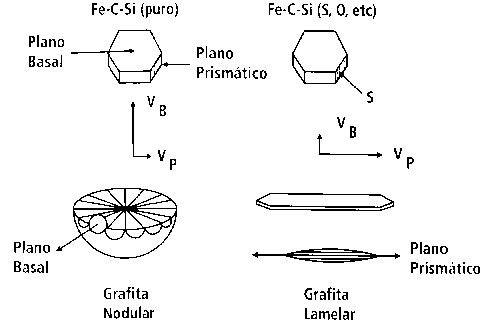
\includegraphics[width=10cm]{img/grafita.pdf}
  \caption{Esquema de crescimento da grafita nas direções normais aos planos basais e prismáticos. Adaptado de\cite{McSwain1975}.}
  \label{fig:grafita}
\end{figure}

É comum a prática de inoculação do ferro fundido com elementos de ação grafitizante pouco antes do vazamento do metal líquido, com o objetivo diminuir o super-resfriamento para o início da formação da grafita e, assim, evitar que o eutético metaestável seja formado\cite{Santos1989}. O grau de inoculação de ferros fundidos nodulares controla a dispersão dos nódulos de grafita no metal e, consequentemente, também o espaçamento entre as células eutéticas.

\subsection{Solidificação}

Em um primeiro momento, a solidificação de ferros fundidos pode ser avaliada de acordo com as reações dos eutéticos estável $\text{líquido} \rightarrow \text{austenita} + \text{grafita}$ e metaestável $\text{líquido} \rightarrow \text{austenita} + \text{cementita}$. A composição química e a velocidade de resfriamento são os principais parâmetros que definem a natureza da reação eutética nos ferros fundidos. Enquanto no sistema Fe-C a diferença entre as temperaturas de equilíbrio do eutético estável e metaestável é de aproximadamente \SI{7}{\degreeCelsius} (a temperatura do eutético estável sendo mais elevada), em uma liga Fe-Si-C contendo 2\% em massa de silício essa diferença é de $\approx$~\SI{35}{\degreeCelsius}\cite{Santos1989}. O elementos que possuem a propriedade de aumentar a diferença entre os dois eutéticos, como o próprio silício, alumínio, níquel e cobre, são classificados como elementos grafitizantes. Por outro lado, elementos que são fortes formadores de carbonetos, como o cromo, vanádio e o tungstênio tendem a aproximar as temperaturas dos dois eutéticos. Por esta propriedade, são geralmente empregados na produção de ferros fundidos brancos. Altas taxas de resfriamento favorecem a formação do eutético metaestável, uma vez que a formação da cementita é mais rápida do que a precipitação da grafita.

A solidificação do ferro fundido nodular começa com a formação da fase primária de solidificação a partir do líquido, que pode ser tanto a austenita, quanto a grafita, dependendo se a composição da liga for hipo ou hipereutética, respectivamente. Em ambos os casos, conforme a fase primária é formada a composição do líquido se aproxima da composição do ponto eutético. Em seguida, a fase líquida se solidifica de acordo com a reação do eutético estável. Embora ainda hajam várias questões em aberto em relação à exata sequência de etapas durante a reação eutética em ferros fundidos nodulares, \citaremsentenca{Polackzek2008} apontam que resultados recentes mostram que há as dendritas de austenita possuem um papel importante na solidificação eutética, de modo que a sequência de solidificação é descrita de acordo com as seguintes etapas:

\begin{itemize}
  \item Na temperatura eutética, dendritas de austenita e nódulos de grafita nucleam independentemente no líquido
  \item Crescimento limitado dos nódulos ocorre em contato com o líquido
  \item Convecção ou flotação determinar a colisão dos nódulos de grafita com as dendritas de austenita
  \item Encapsulamento da grafita pela austenita ocorre antes ou imediatamente após o contato entre a grafita e as dendritas de austenita
  \item Posterior crescimento da grafita ocorre pela difusão de carbono através do invólucro de austenita
\end{itemize}

\citaremsentenca{Ruxanda2001} ainda reportam a existência de múltiplos nódulos de grafita dentro de um grão de austenita e que o crescimento da fase austenita na célula eutética é controlado pela difusão de carbono, enquanto que o crescimento da grafita é controlado pela auto-difusão dos átomos de ferro, uma vez que a grafita necessita de espaço para expandir em direção ao sólido adjacente. A sequência de solidificação eutética do ferro fundido nodular é mostrada esquematicamente na Figura \ref{fig:eutetico_nodular}.

\begin{figure}
  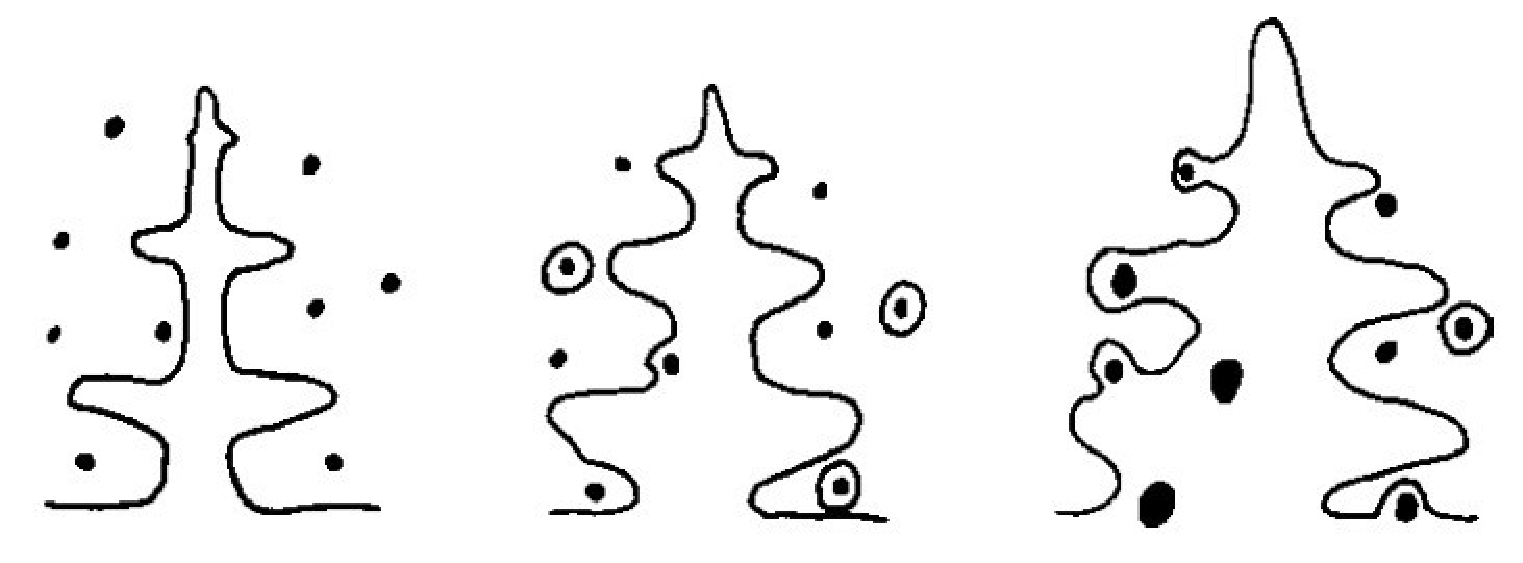
\includegraphics[width=.7\textwidth]{img/eutetico_nodular.pdf}
  \caption{Desenho esquemático ilustrando a sequência da solidificação eutética em um ferro fundido nodular\cite{Polackzek2008}.}
  \label{fig:eutetico_nodular}
\end{figure}

A reação eutética no ferro fundido nodular é essencialmente diferente de outras formas de solidificação eutética em outros ferros fundidos, como o cinzento. No ferro fundido cinzento o crescimento da célula eutética a austenita e a grafita de morfologia lamelar crescem cooperativamente, enquanto que o eutético no ferro fundido nodular é do tipo divorciado, sem o crescimento acoplado de duas fases na interface sólido/líquido\cite{Santos1989,Polackzek2008}.

% Por outro lado, as etapas da solidificação de acordo com o eutético estável em ferros fundidos nodulares ainda não é completamente entendida. Segundo \citaremsentenca{Ruxanda2001}, embora pesquisadores concordem que a nucleação de tanto a austenita quando a grafita ocorre no líquido, há diversas opiniões em relação à sequência de nucleação (se ou a grafita ou a austenita nucleam primeiro) e sobre a exata localização da nucleação das fases (aleatória ou em sítios preferenciais). Stefanescu postulou a

% Em ferros nodulares de composição eutética, a solidificação se inicia quando o metal líquido é su\-per-res\-fri\-a\-do a temperaturas inferiores à do eutético estável, quando se dá a nucleação e crescimento dos nódulos de grafita. Na sequência, os nódulos formados são encapsulados por um invólucro de austenita, formando a denominada célula eutética. As células eutéticas continuam crescendo até que todo o calor latente da solidificação seja liberado e a solidificação tenha chegado a seu fim\cite{Santos1989}. %Vide\cite{Stefanescu2005} para citar Patterson e Scheil (1949)


% Em ligas hipoeutéticas e hipereutéticas, por sua vez, há a formação de uma fase primária no início da solidificação. No primeiro caso, a solidificação se inicia com a formação de dendritas de austenita, enquanto no segundo caso nódulos de grafita são formados diretamente a partir do líquido. Em ambos os casos, na medida em que o material é resfriado, a composição do líquido progressivamente se aproxima da composição eutética. A reação eutética, no entanto, só se inicia uma vez atingido um super-resfriamento suficiente para nucleação e crescimento dos nódulos de grafita\cite{Santos1989}.

Vale mencionar que na microestrutura final das ligas eutética e hipoeutética de ferros fundidos nodulares é normalmente observada uma população de nódulos de grafita com tamanhos dispersos segundo uma distribuição normal. Em ligas hipereutéticas, por sua vez, são observadas duas diferentes populações de nódulos de grafita: uma cuja média dos diâmetros é maior, correspondente aos nódulos primários de grafita, formados entre as temperaturas \enfase{liquidus} e do eutético metaestável, e outra cujo tamanho médio da população é menor, formada durante a reação eutética\cite{Santos1989}. %citar quem o Santos cita


\subsubsection{Microssegregação de elementos durante a solidificação}

Microssegregação é o termo que define a condição de não-uniformidade de composição química no material a nível microestrutural. Em complemento à definição de microssegregação, macrossegregação trata-se da não-uniformidade de composição química em larga escala, comparável ao tamanho da peça. 
% A macrosegregação é um defeito do processo de fundição do metal e, portanto, seu controle possui caráter tecnológico. 
% Por outro lado, a microssegregação é inerente ao produto fundido e, dessa forma, tem sua devida importância reconhecida nesta seção do texto.

A microssegregação se origina devido à expulsão de soluto da fase sólida ao crescer a partir do metal líquido. Caso a liga seja resfriada lentamente, o contato prolongado entre líquido e sólido permitirá a difusão de soluto até o estabelecimento do equilíbrio termodinâmico para cada temperatura. No entanto, nas situações reais, em que taxas de resfriamento elevadas são impostas ao material, a partição de soluto entre as fase sólida e líquida causa uma heterogeneidade de composição ao final da solidificação. Dessa forma, na microestrutura bruta de fundição há a preponderância do soluto nas últimas porções de metal a se solidificar.

Em ferros fundidos a microssegregação também é originada na formação da fase de solidificação primária, mas é principalmente atribuída à reação eutética. Como estas ligas possuem ao menos três elementos químicos, a regra das fases de Gibbs\footnotemark{} prevê que a reação eutética $\text{líquido} \rightarrow \text{austenita} + \text{grafita}$ não ocorre em um ponto invariante, mas sim em uma faixa de temperaturas. Devido às limitadas difusividades dos elementos na fase sólida e à dependência de suas solubilidades em relação à temperatura de solidificação, ocorre que as sucessivas camadas de austenita formadas a partir do líquido apresentam diferentes composições químicas. Assim, elementos que apresentam maior solubilidade na austenita do que na fase líquida em temperaturas mais elevadas, como silício, níquel e cobre, tendem a se concentrar nas primeiras regiões a se solidificar. Na formação do eutético divorciado do ferro nodular, portanto, estes elementos se concentrarem próximos aos nódulos de grafita. Por outro lado, carbono, enxofre, manganês, cromo e molibdênio são rejeitados da austenita para líquido e acabam permanecendo em maior concentração nas últimas regiões a se solidificar, isto é, aquelas que correspondem ao encontro das células eutéticas. %Referenciar e inserir figura

\footnotetext{A regra das fases foi proposta por J.W. Gibbs em seu famoso trabalho de 1878 \enfase{On the Equilibrium of Heterogeneous Substances}\cite{Gibbs1878}. A equação estabelece a igualdade $F = C - P + 2$, em que $F$ é o número de graus de liberdade (número de variáveis de estado independentes), $C$ o número de componentes do sistema e $P$ o número de fases. Para um sistema constituído apenas de fases condensadas, em que o efeito da pressão é desprezível, pode ser simplificado para $F = C - P + 1$.}

Uma ferramenta muito útil para o entendimento e quantificação (estimativa) da microssegregação é o modelo de Scheil-Gulliver. %\cite{Porter2009}
A equação desenvolvida por Scheil apud \citaremsentenca{Porter2009} %pegar referência original do Scheil?
vale para uma liga binária cuja solidificação gera apenas uma fase sólida. As hipóteses de Scheil representam a situação de máxima segregação, em que a difusão do soluto na fase sólida é completamente desprezada e, portanto, não é possível o estabelecimento do equilíbrio termodinâmico em todo o sistema. As considerações feitas neste modelo são:

\begin{enumerate}
  \item Não há difusão na fase sólida após sua formação;
  \item A difusão é infinitamente rápida na fase líquida para todas as temperaturas. Essa ponderação é equivalente a considerar a composição química homogênea ao longo de todo o líquido;
  \item As composições na interface sólido-líquido são de equilíbrio, valendo as composições preditas pelo diagrama de fases em uma dada temperatura. Essa hipótese não significa que há o estabelecimento do equilíbrio no sistema, mas \enfase{apenas} na interface. Ela é semelhante à adotada por Zener para transformações difusionais em estado sólido (vide seção \ref{sec:consTransf});
  \item As linhas \enfase{solidus} e \enfase{liquidus} são representadas por linhas retas no diagrama de fases. \label{item:scheil4}
\end{enumerate}

Postas estas condições, define-se o coeficiente de partição $k$, que corresponde à razão entre o teor de soluto $C_S$ na fase sólida a composição química $C_L$ na fase líquida, ambos determinados pelo diagrama de fases:

\begin{subequations}
  \begin{align}
    \label{eq:coefPart}k = \frac{C_S}{C_L}
  \end{align}
\end{subequations}

Note-se que, devido à hipótese \ref{item:scheil4}, $k$ assume valor constante. Atualmente, graças ao aumento do poder computacional e ao desenvolvimento de bases de dados termodinâmicos, esta hipótese pode ser relaxada utilizando técnicas numéricas, tais quais as empregadas nos softwares que empregam o método CALPHAD. %pacote de software? protocolo? não sei direito o que é o CALPHAD

\novasiglaestrangeira{CALPHAD}{Computer Coupling of Phase Diagrams and Thermochemistry} %Prestar atenção se fica dentro ou fora da ordem alfabética.

As demais equações que definem o problema consistem da condição inicial de solidificação (equação \ref{eq:condIni}), isto é, que a composição do líquido no início da solidificação é igual à composição média da liga $C_0$, a conservação de massa do sistema (equação \ref{eq:balSis}), dada pela soma unitária das frações de sólido ($f_S$) e líquido ($f_L$), e o balanço de massa na interface (equação \ref{eq:Stefan}), que corresponde ao balanço entre a redistribuição do soluto e o aumento da fração de sólido.

\begin{subequations}[resume]
  \begin{align}
    \label{eq:condIni}\left.C_L\right|_{f_S=0} &= C_0\\
    \label{eq:balSis}f_S + f_L &= 1\\
    \label{eq:Stefan}\left(C_L - C_S\right) df_S &= f_L dC_L
  \end{align}
\end{subequations}

A integração da equação diferencial \ref{eq:Stefan} nos domínios de integração definidos pela condição inicial (equação \ref{eq:condIni}) utilizando as substituições dos termos adequados obtidos pelas equações \ref{eq:coefPart} e \ref{eq:balSis} leva à equação de Scheil-Gulliver para composição do sólido e do líquido durante a solidificação:

\begin{subequations}
  \begin{align}
    C_L &= C_0 {f_L}^{k-1}\\
    \label{eq:C_S}C_S &= k C_0\left(1 - f_S\right)^{k-1}
  \end{align}
\end{subequations}

Graças ao desenvolvimento de bases de dados termodinâmicas é possível também utilizar as considerações de Scheil para estimar a microssegregação durante a solidificação de ligas multicomponentes, que frequentemente geram mais de uma fase sólida diretamente do líquido. Softwares que seguem o método CALPHAD, como o Thermo-Calc\textregistered, possuem módulos que permitem esse tipo de contabilização. Adicionalmente, quando acoplados com informações sobre a difusividade dos elementos químicos, também permitem a utilização de condições de equilíbrio parcial na interface (tais quais as apresentadas na seção \ref{sec:consTransf}) e aplicação de difusão no estado sólido\cite{Chen2002,Larouche2007}.

\subsection{Transformações no estado sólido}

Durante o resfriamento lento do metal solidificado, em torno de \SI{720}{\degreeCelsius} ocorre a decomposição eutetóide da austenita, que, assim como a reação eutética, pode acontecer na forma estável ($\text{austenita} \rightarrow \text{ferrita} + \text{grafita}$) ou metaestável ($\text{austenita} \rightarrow \text{ferrita} + \text{cementita}$). A predominância de uma reação ou outra é novamente dependente da taxa de resfriamento e da composição química, além da distância entre as partículas de grafita.

Durante a reação do eutetóide estável, a austenita se decompõe em ferrita e grafita secundária. A nucleação da ferrita se dá preferencialmente na interface entre a austenita e os nódulos de grafita formados durante a solidificação. A ferrita cresce para o interior da austenita, enquanto a grafita é incorporada aos nódulos pré-existentes. Em estágios avançados da reação a ferrita engloba completamente o nódulo, formando uma barreira para a difusão de carbono da austenita para a grafita, diminuindo substancialmente a velocidade da reação. A tendência a partir desse ponto é que a reação do eutetóide metaestável, que corresponde à decomposição da austenita em perlita, predomine e consuma a austenita não-transformada. A Figura \ref{fig:matriz_fofo} ilustra a sequência de etapas da decomposição eutetóide da austenita.

\begin{figure}
  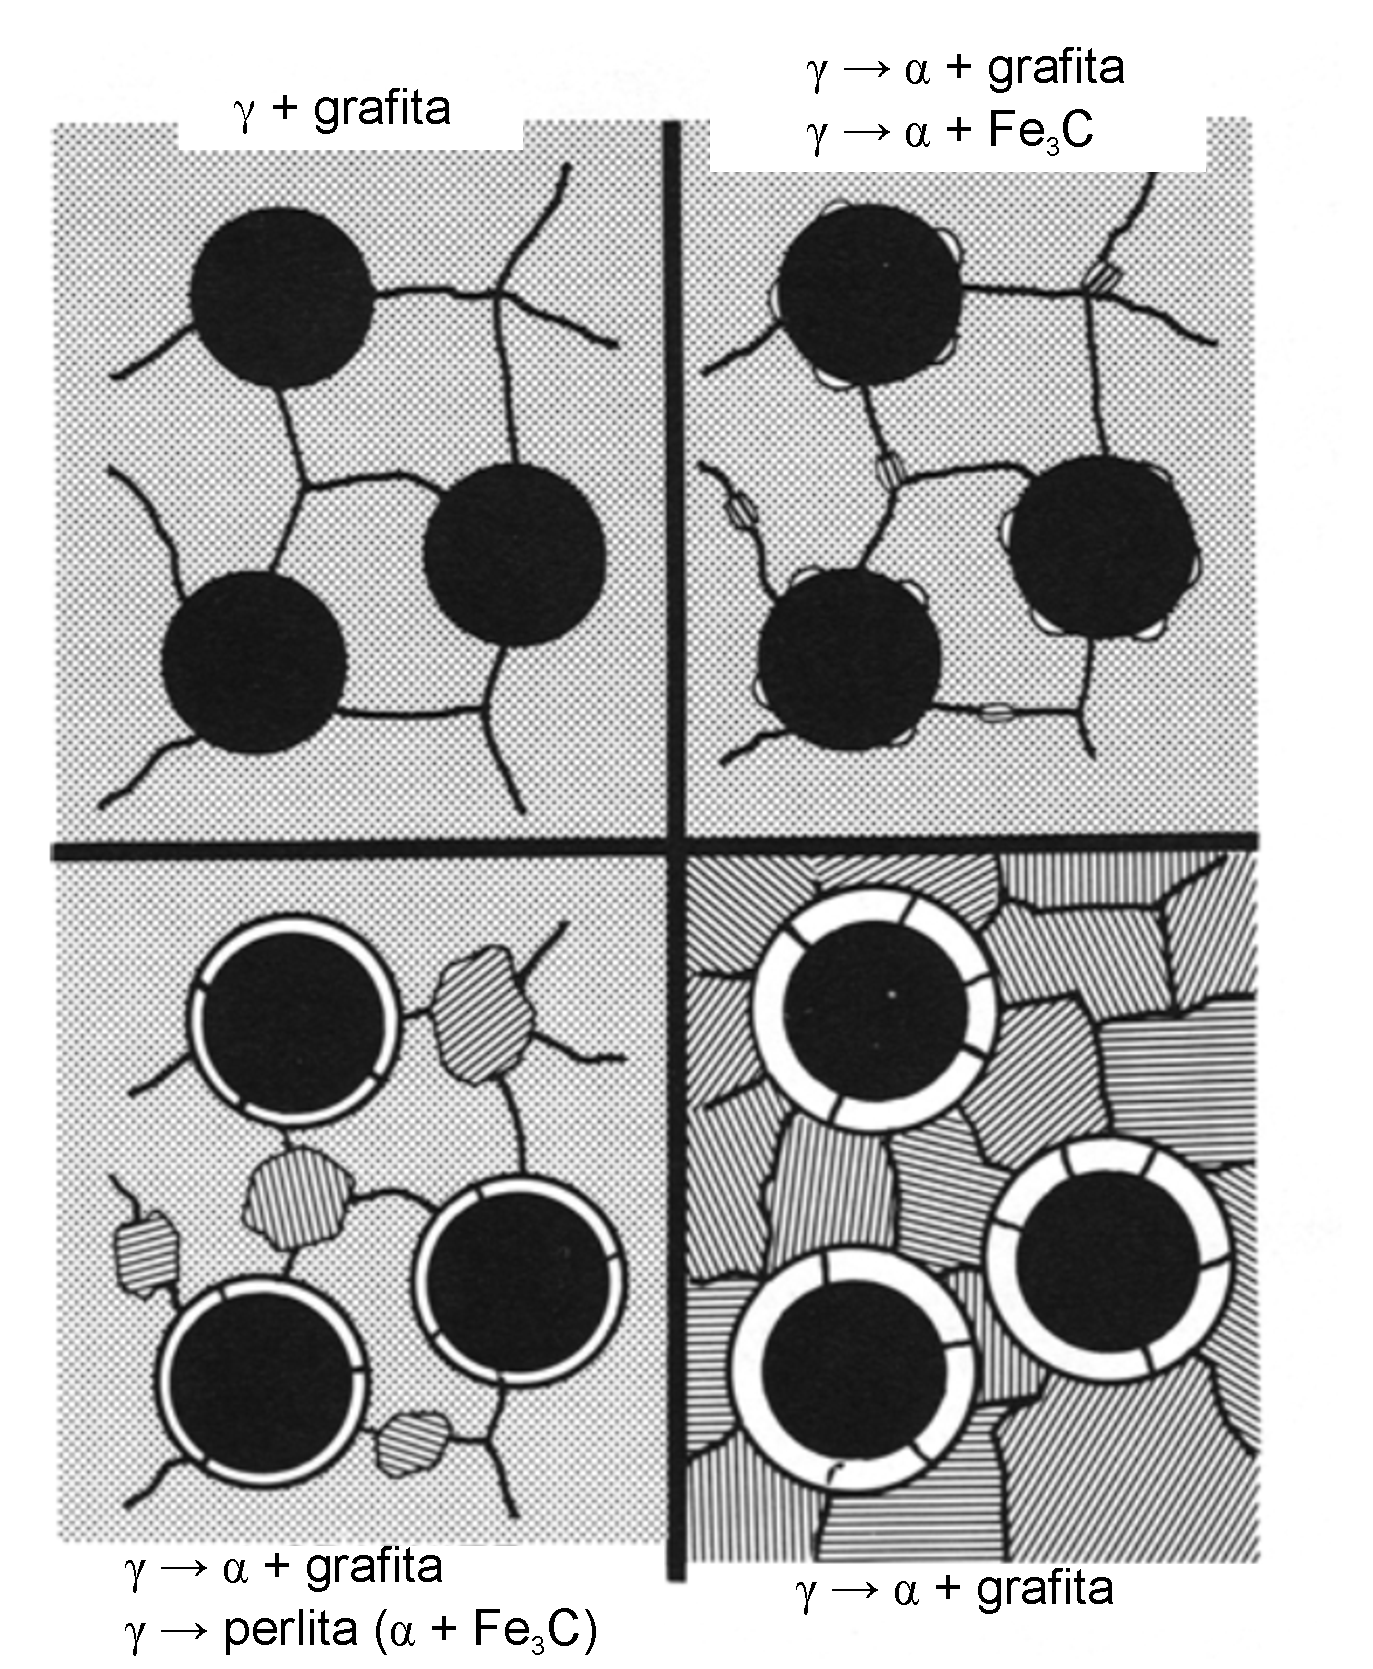
\includegraphics[width=.6\textwidth]{img/matrizFofo.pdf}
  \caption{Ilustração esquematizando a decomposição eutetóide em ferros fundidos nodulares\cite{Johnson1978}.}
  \label{fig:matriz_fofo}
\end{figure}

A perlita consiste de um agregado de lamelas alternadas de ferrita e cementita. O crescimento da perlita se dá de forma cooperativa, ou seja, as duas fases crescem simultaneamente. Ao contrário da precipitação de grafita no estado sólido, a formação de cementita não requer difusão a longo alcance dos átomos de Fe. Por este motivo, para uma ampla faixa de temperaturas a cinética da reação perlítica é consideravelmente mais rápida do que a formação do eutetóide estável. \citaremsentenca{Zener1946} estudou a cinética local de crescimento da perlita assumindo que a distância de difusão característica de seu crescimento seria o espaçamento interlamelar. Em consequência, Zener concluiu que a velocidade de crescimento de uma colônia é constante e independente da porção transformada da austenita, ao contrário do que acontece no eutetóide estável.

Elementos como antimônio, cobre e estanho são chamados de ``perlitizantes'' por atuarem evitando a formação da ferrita oriunda do eutetóide estável\cite{Kovacs1981}.
A obtenção de uma matriz perlítica também pode ser conseguida por meio de tratamentos térmicos, como é o caso da normalização. Matrizes completamente ferríticas também podem ser obtidas por meio tratamentos térmicos. O recozimento é um tratamento térmico em que a peça é aquecida a temperaturas próximas à de início de eutetóide estável que leva à dissociação da perlita para formação da estrutura de equilíbrio ferrita + grafita\cite{Guesser2009}.

Além das matrizes ferrítica e perlítica convencionais, ferros fundidos podem ser submetidos a tratamentos de têmpera, para obtenção de uma matriz martensítica, e austêmpera, para obtenção de matriz constituída de bainita isenta de carbonetos e austenita retida estabilizada por carbono. Estas matrizes conferem ao material resistência mecânica muito superiores às matrizes ferrítica e perlítica e, no caso do produto austemperado, elevadas ductilidade e tenacidade ao impacto\cite{Guesser2009}.


\subsection{Ferro fundido nodular austemperado (ADI)}

\label{subsec:ADI}

Em aços carbono, tratamentos isotérmicos aplicados à austenita em temperaturas inferiores às de formação da perlita geram um microconstituinte eutetóide denominado bainita. Morfologicamente, a bainita se apresenta na forma de ripas de ferrita (ou agulhas, como é visto em uma seção bidimensional) contendo carbonetos dispersos entre cada unidade de ferrita (bainita superior), ou em seu interior (bainita inferior).

Em ligas ferrosas contendo silício a transformação bainítica possui uma cinética característica, consistindo de uma etapa inicial de formação de feixes de ferrita bainítica (também referenciada como ferrita pró-bainítica e bainita isenta de carbonetos), seguida por um período de estagnação conhecido como ``estase'', para que a reação, enfim, possa ser retomada pela precipitação de carbonetos nas ilhas de austentita não-transformadas\cite{Goldenstein2002}. %ESCOLHER MELHOR REFERENCIA
Durante a primeira etapa da reação nestas ligas, a ferrita bainítica progressivamente enriquece em carbono a austenita adjacente. Como será discutido na seção \ref{sec:Martensita} deste trabalho, austenita com teores elevados de carbono possui pouca tendência de se transformar durante o resfriamento. Assim, dependendo do enriquecimento em carbono da austenita durante a transformação baínitica interrompida, uma grande quantidade de austenita pode ser estabilizada à temperatura ambiente.

O ferro fundido nodular austemperado (do inglês, \siglaestrangeira{ADI}{Austempered Ductile Iron}) faz uso desse fenômeno para obtenção de uma matriz bifásica de finas ripas de ferrita intercaladas com filmes ou blocos de austenita --- produto chamado de ``ausferrita'' na literatura de fundição. Nos ferros fundidos o fenômeno da estase é prolongado devido aos elevados teores de silício inerentes a esse material. Ainda assim, o processo é somente viável em uma ``janela de processo'', que corresponde ao intervalo de tempos e temperaturas em que o produto austemperado confere propriedades dentro das faixas de propriedades estabelecidas pela norma ASTM A897\cite{Bayati1999,A04Committee2016} e normalmente termina com a precipitação de carbonetos na reação bainítica. Quando produzida nos parâmetros adequados de tratamento térmico, a ausferrita confere ao ADI elevada resistência mecânica aliada a elevada ductilidade devido à ocorrência do efeito TRIP (\enfase{Transformation Induced Plasticity})\cite{Goldenstein2002}. Por este motivo, o ADI proporciona propriedades comparáveis às obtidas em aços, em algumas situações se mostrando favoravelmente competitivo por agregar as vantagens de produção próxima da forma final (\enfase{near-net-shape}) decorrente do processo de fundição\cite{Trudel1997,Hayrynen2002}.

O tratamento térmico para produção do ADI, ilustrado na Figura \ref{fig:austemperaMeier}, consiste de uma etapa inicial de aquecimento até o campo de equilíbrio de austenita e grafita (austenitização), na qual o material é mantido durante um determinado tempo. Em seguida, as peças são mergulhadas em banho de sal fundido, pré-aquecido na temperatura de austêmpera, onde são mantidas por tempo suficiente longo para que a austenita enriquecida em carbono seja retida à temperatura ambiente\cite{Trudel1997}.

\begin{figure}
  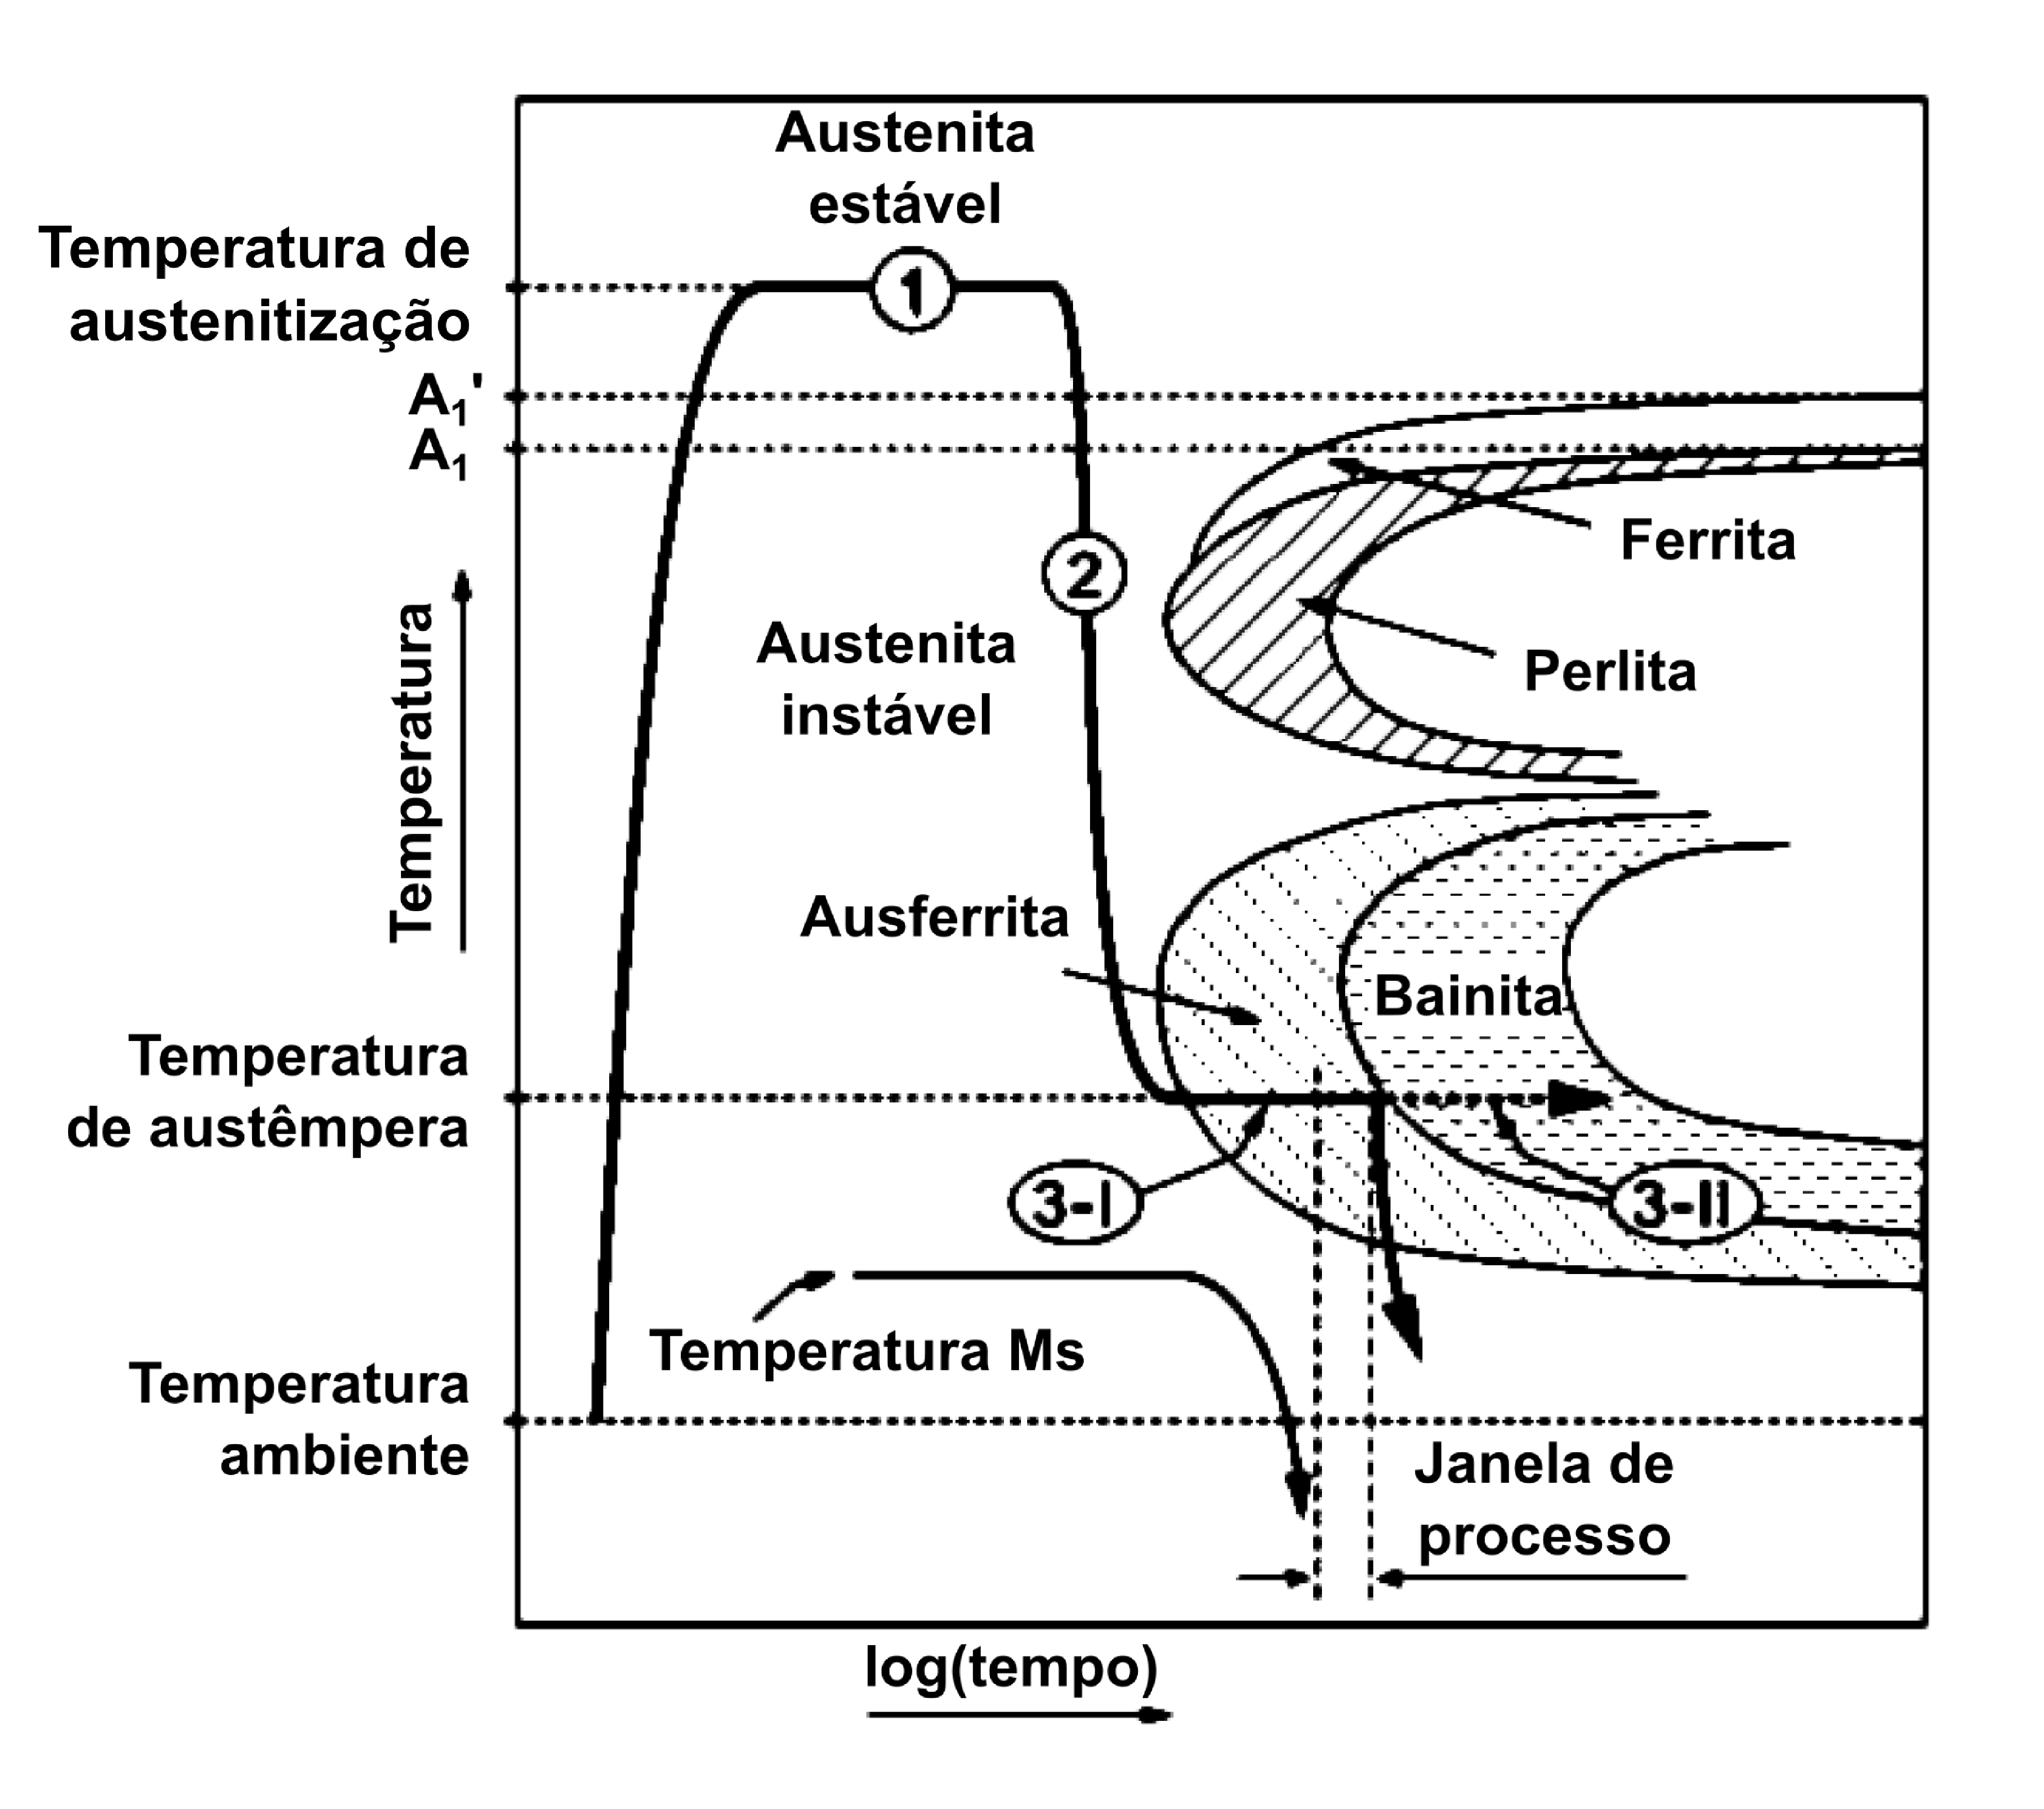
\includegraphics[height=10cm]{img/austemperaTTT_Meier.pdf}
  \caption{Diagrama TTT esquemático ilustrando o processo de austêmpera de ferros fundidos\cite{Meier2013a}.}
  \label{fig:austemperaMeier}
\end{figure}

A temperatura de austenitização controla a composição da austenita em equilíbrio com a grafita. Temperaturas mais elevadas ajudam na homogeneização dos elementos de liga microssegregados e a maior dissolução da grafita, conferindo um maior teor de carbono à austenita e, portanto, também maior temperabilidade ao material. A elevada temperabilidade confere menor tendência de formação de perlita durante o resfriamento, indesejável para o alcance das propriedades mecânicas\cite{Trudel1997}. Além disso, tempos mais prolongados de austêmpera seriam necessários para o início da transformação bainítica e, uma vez estabelecido o final da primeira etapa da reação, maiores frações de austenita retida acabariam sendo obtidas. O uso intensivo de elementos químicos produz efeito semelhante sobre a temperabilidade do material, mas deve ser utilizado com especial cuidado devido aos problemas associados à microssegregação\cite{Bayati1995,Velez1996}. \citaremsentenca{Trudel1997} apontam que o tempo de austenitização deve ser o mínimo possível para que garantir que o material se transforme completamente em austenita saturada em carbono e grafita, sendo o tempo de uma hora à temperatura de \SI{900}{\degreeCelsius} em uma peça de \SI{25}{mm} de diâmetro geralmente suficiente para garantir isso. No entanto, para temperaturas mais baixas, tempos superiores a três horas podem ser necessários para a eliminação das heterogeneidades de composição química.

A temperatura de austêmpera desempenha um papel importante no estabelecimento das propriedades mecânicas do ADI. Temperaturas elevadas levam à formação de um produto com excelente ductilidade e resistência a esforços dinâmicos, enquanto temperaturas baixas geram um produto extremamente resistente ao desgaste\cite{Lin1996,Aranzabal1997,Magalhaes1998}. Microestruturalmente, a ausferrita formada em duas temperaturas diferentes apresenta mudanças significativas. Como pode ser observado na Figura \ref{fig:ADIs}a, o material tratado termicamente a \SI{360}{\degreeCelsius} apresenta ripas grosseiras de bainita com grandes quantidades de austenita, enquanto ADI produzido a \SI{310}{\degreeCelsius} possui uma microestrutura mais refinada, composta de menores ilhas de austenita isoladas umas das outras.

\begin{figure}
  \subfloat[]{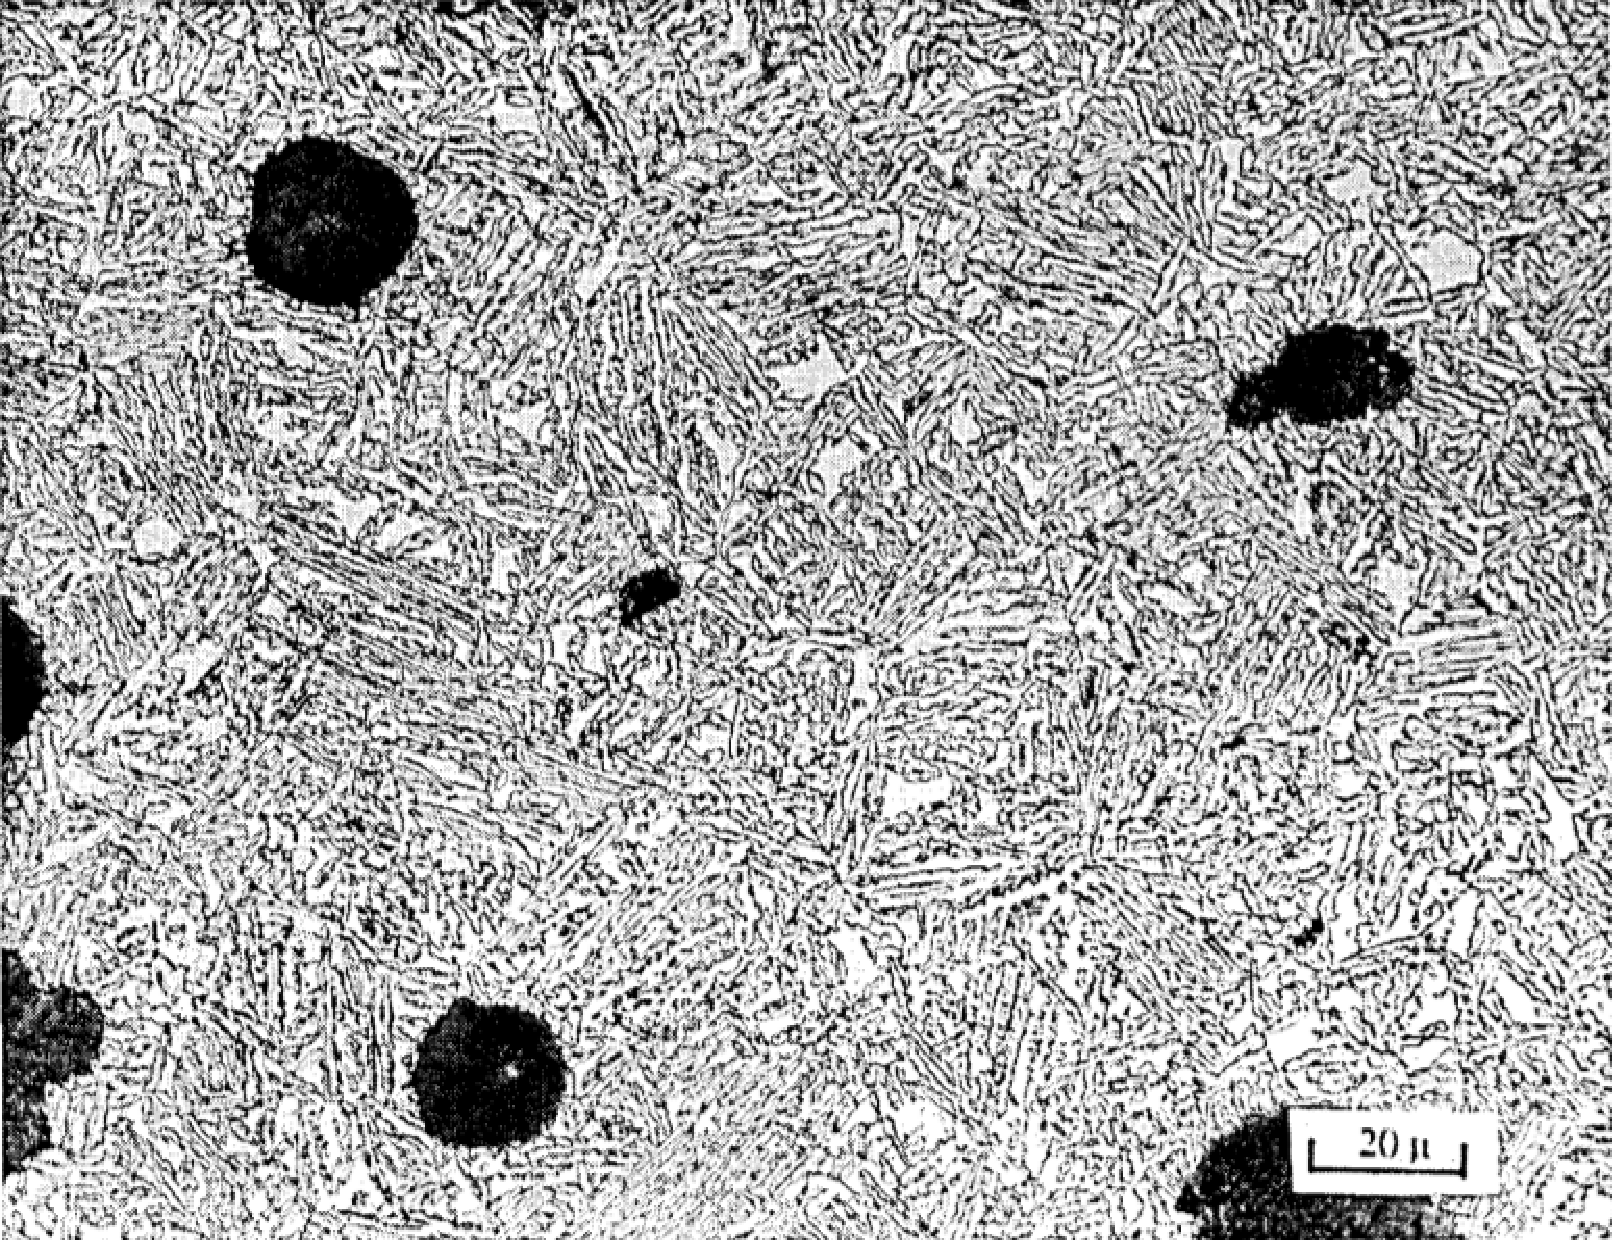
\includegraphics[height=5.8cm]{img/ADI360oC.pdf}}
  \quad
  \subfloat[]{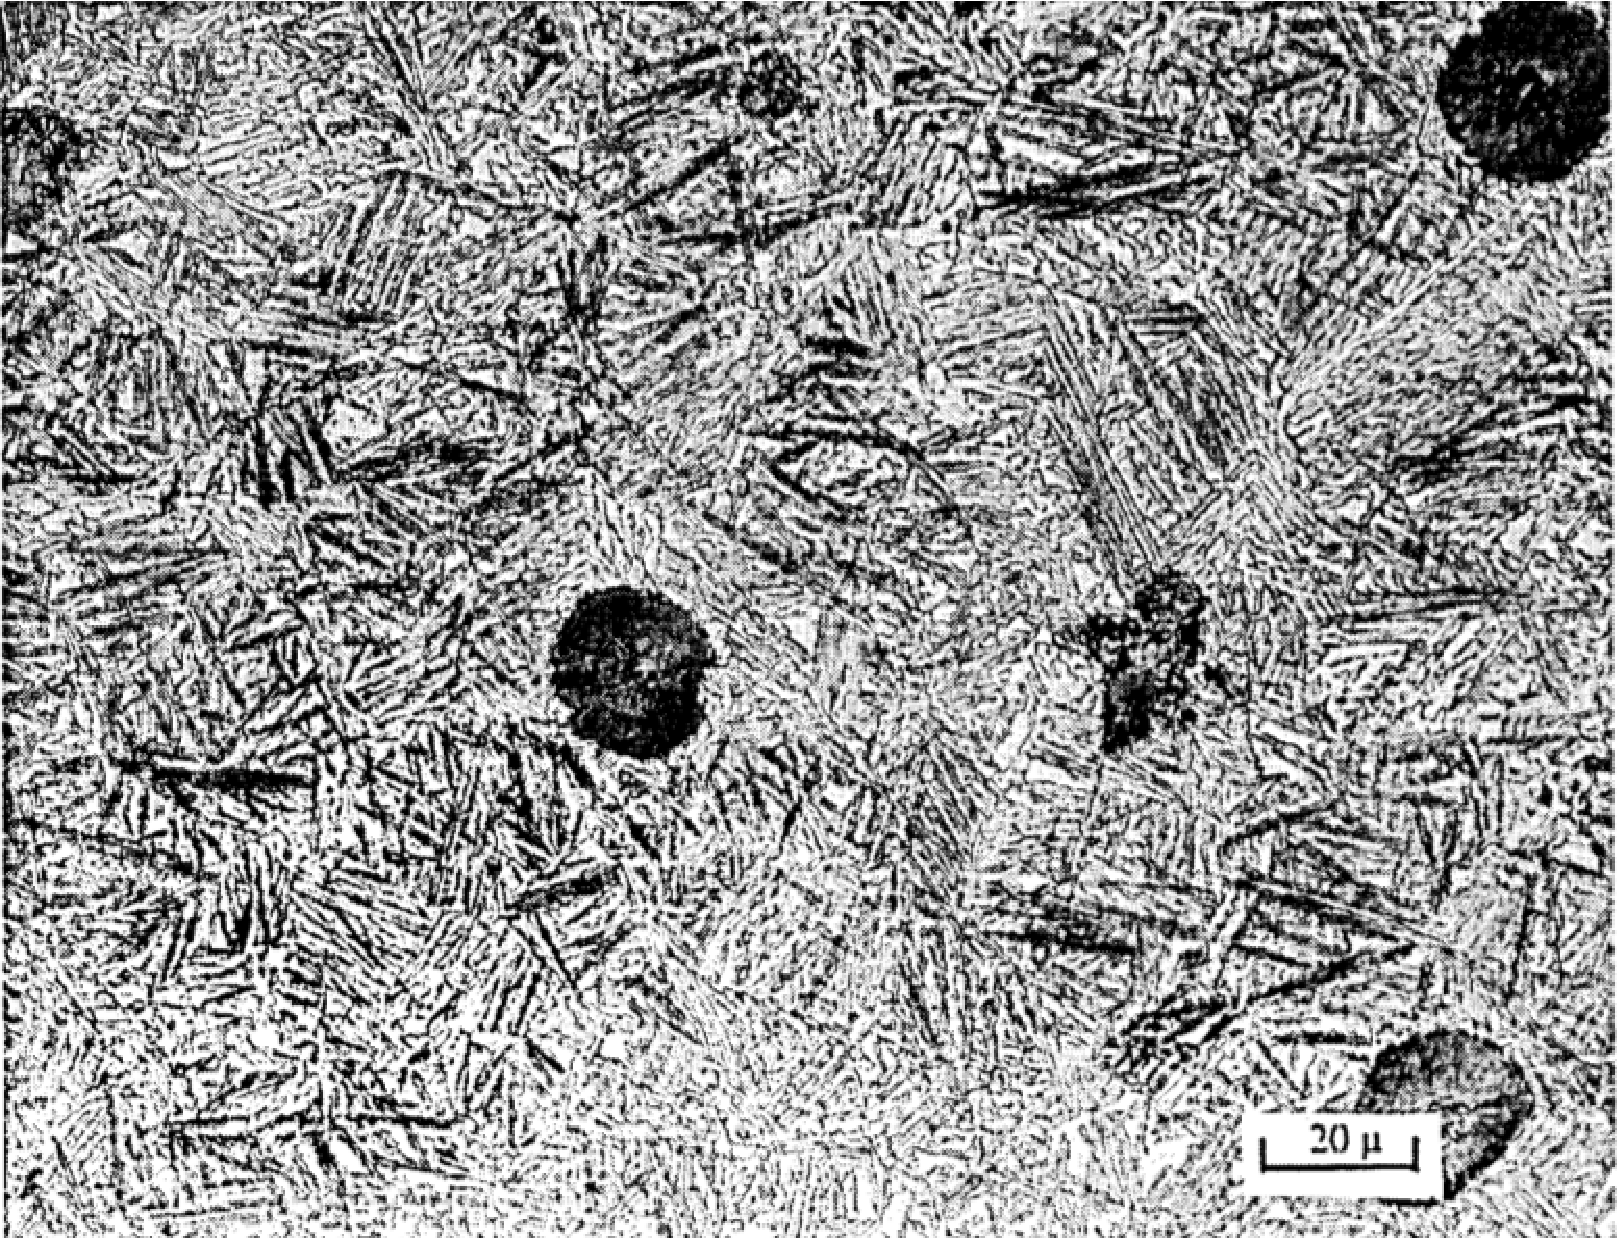
\includegraphics[height=5.8cm]{img/ADI310oC.pdf}}
  \caption{Microestruturas de ADIs produzidos pela austêmpera a (a) \SI{360}{\degreeCelsius} e (b) \SI{310}{\degreeCelsius} por uma hora. Imagens reproduzidas de\cite{Trudel1997}.}
  \label{fig:ADIs}
\end{figure}

Um aspecto importante da produção do ADI é o efeito da microssegregação na transformação bainítica no material. Como mencionado anteriormente, alguns autores reportam que é conveniente eliminar a microssegregação durante a etapa de austenitização. A justificativa para aplicação de tal medida é ilustrada na Figura \ref{fig:cineticaADI}, que mostra esquematicamente o crescimento das colônias de ausferrita no ferro fundido. Devido à segregação nos contornos de células eutéticas, estas regiões possuem maior temperabilidade e, consequentemente, apresentam cinética mais lenta de transformação. \citaremsentenca{Trudel1997} reportam que a austenita nestas regiões, por não se transformar, fica empobrecida em carbono e pode não se manter totalmente estabilizada à temperatura ambiente, transformado-se parcialmente em martensita. \citaremsentenca{Bayati1995} mostraram que em um ferro nodular contendo 0,67\% de manganês, devido à diferença entre as cinéticas de transformação nas duas regiões, ocorre a superposição das etapas de transformação da ausferrita. Isto é, enquanto a austenita nas regiões intercelulares ainda estão enriquecendo em carbono pelo primeiro estágio da reação, a precipitação de carbonetos já se inicia nas regiões em que a transformação começara primeiro. Este fenômeno leva à diminuição da janela de processo do material. \citaremsentenca{Meier2013a} fizeram observações semelhantes por meio de difração de nêutrons \enfase{in situ} e mostraram que a formação da ausferrita é associada a uma assimetria dos picos de difração da austenita, atribuída a fases com cinéticas de transformação diferentes.

\begin{figure}
  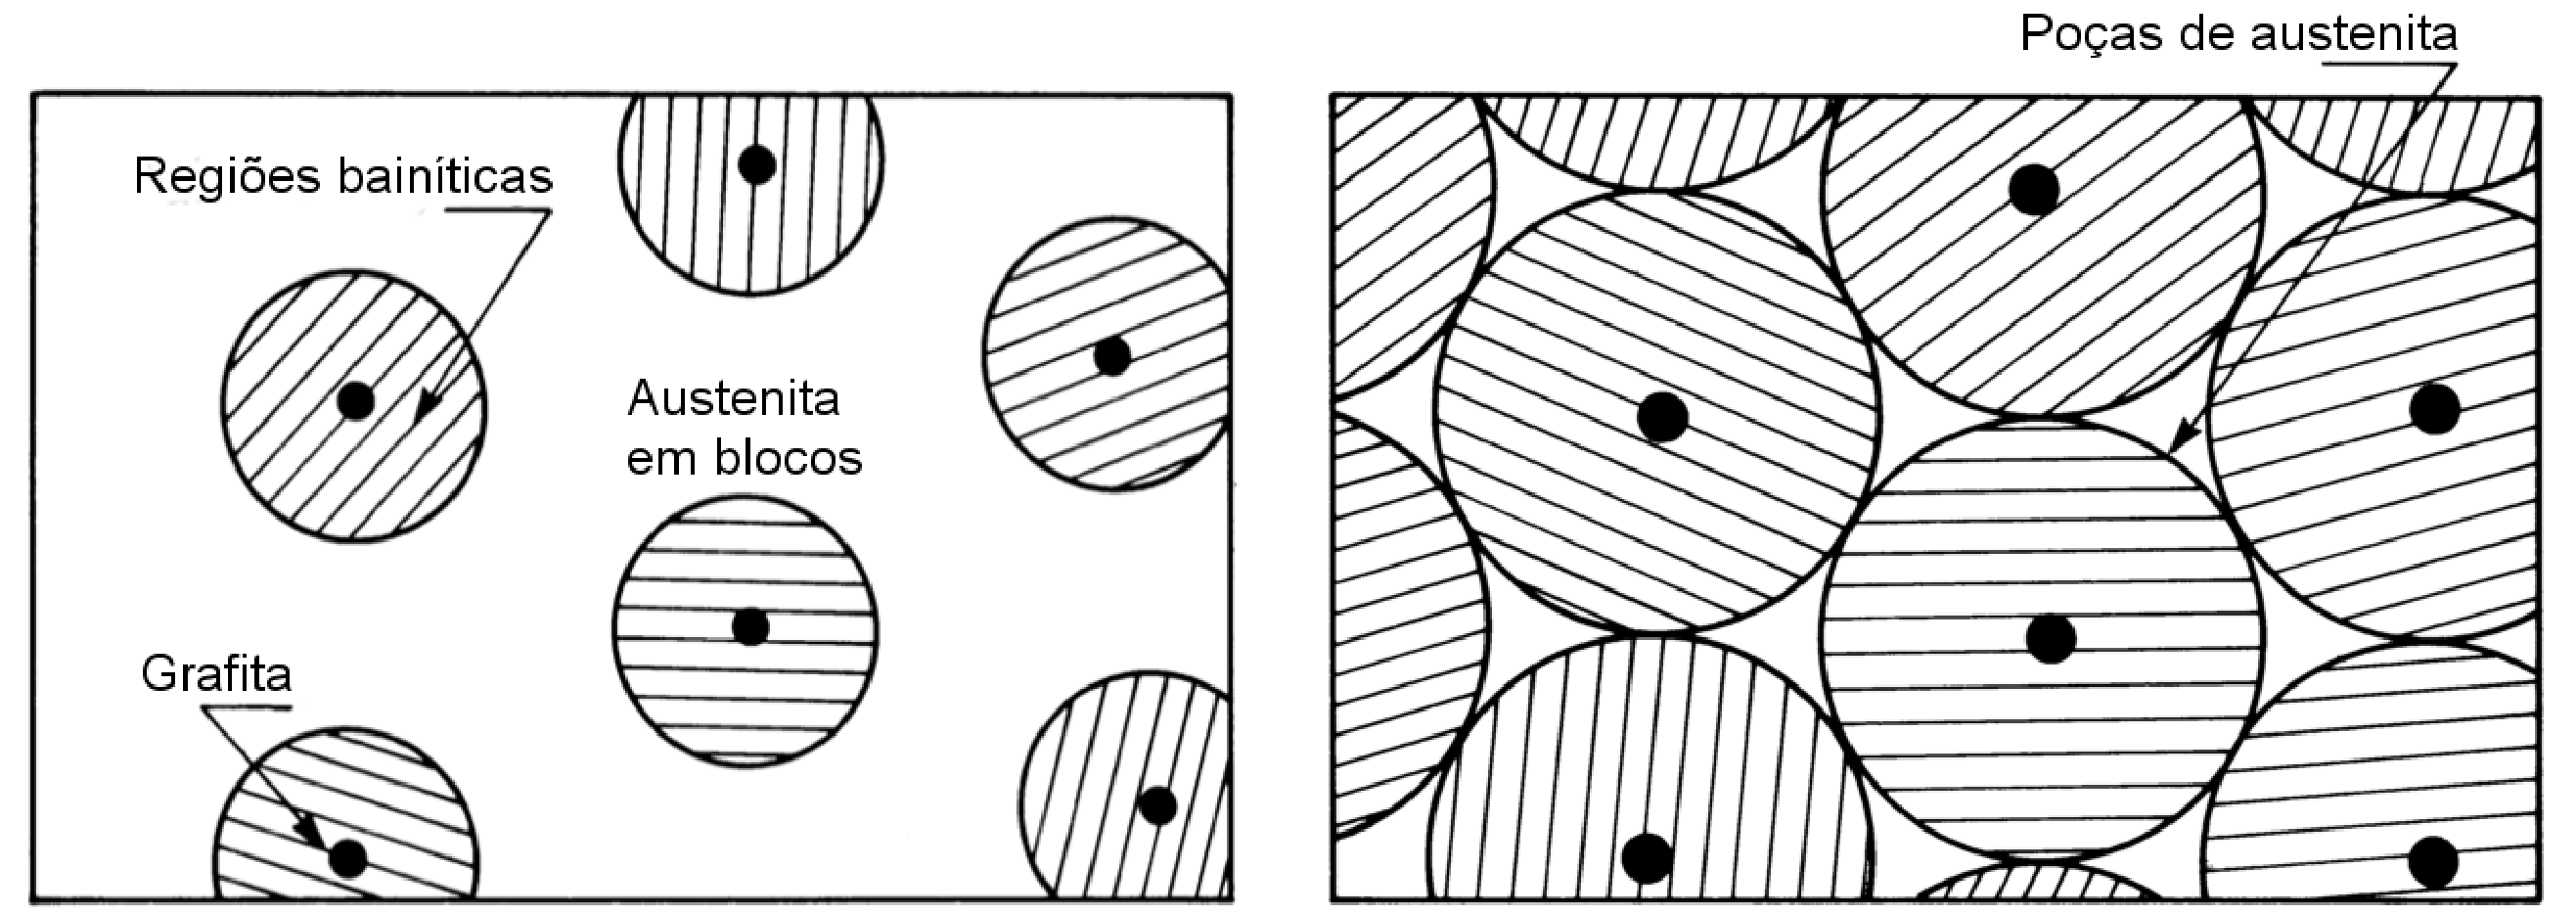
\includegraphics[width=16cm]{img/crescimentoAusferrita.pdf}
  \caption{Esquema representando, de forma bastante simplificada, a evolução da formação de ausferrita em um ADI. A região hachurada corresponde à estrutura de ferrita bainítica entremeada por filmes de austenita enriquecida em carbono. As últimas poças não-trasformadas de austenita geralmente correspondem a contornos de célula eutética. Adaptado de\cite{Aranzabal1997}.}
  \label{fig:cineticaADI}
\end{figure}


\section{Considerações sobre transformações difusionais em ligas multicomponentes}

\label{sec:consTransf}

O atual desenvolvimento das teorias cinéticas de crescimento difusional de fases é em grande parte creditado ao trabalho pioneiro de \citaremsentenca{Zener1946}. Zener construiu um modelo cinético para o crescimento da ferrita a partir da austenita no sistema Fe-C. Para tanto, supôs que as composições na interface entre matriz e precipitado seriam dadas pelas linhas de solubilidade do diagrama de equilíbrio do sistema. Um tratamento mais completo necessita levar em conta vários elementos de liga, o que implica em um grande aumento de complexidade do problema no ponto de vista de modelamento. Particularmente, quando há a adição de elementos substitucionais, a diferença de mobilidade entre os solutos intersticial e substitucionais acarreta em situações de controle cinético com diferentes características, dependendo das forças motrizes às quais o material está sendo submetido. Assim, dependendo da velocidade da movimentação da interface, convém classificar as condições interfaciais em dois diferentes modos: equilíbrio local e paraequilíbrio.

\subsection{Equilíbrio local (EL)}
  
\novasigla{EL}{Equilíbrio local}

A condição de equilíbrio local é caracterizada pela movimentação lenta da interface, de modo a permitir que o equilíbrio local na interface entre precipitado e matriz seja estabelecido. Trata-se da situação assumida por Zener, em que a igualdade dos potenciais químicos das espécies na interface entre as duas fases em contato é obedecida. A condição termodinâmica de EL no crescimento de ferrita ($\alpha$) a partir da austenita ($\gamma$) é dada por:

\begin{equation}
  \mu_i^\alpha = \mu_i^\gamma
\end{equation}
%
em que $\mu_i$ é o potencial químico do elemento $i$ (C, Mn, Si, Cr, etc) na fase.

No que lhe diz respeito, ainda é possível discernir duas situações de EL, dependendo de como os solutos substitucionais são redistribuídos entre a fase em crescimento e a fase matriz.

Sob baixos super-resfriamentos, ocorre considerável redistribuição dos elementos substitucionais entre as duas fases. Nesta situação, conhecida como equilíbrio local com partição de soluto (EL-P)\novasigla{EL-P}{Equilíbrio local com partição de soluto}, a difusão dos substitucionais, por ser mais lenta do que a difusão dos elementos intersticiais, controla a movimentação da interface. Os perfis de composição na interface para a condição EL-P são mostrados na Figura \ref{fig:modcineticos}a.

Sob forças motrizes maiores, a redistribuição do soluto substitucional entre as duas fases é mínima. Neste cenário, chamado de equilíbrio local com partição desprezível de soluto\novasigla{EL-PD}{Equilíbrio local com partição desprezível de soluto}, a composição das fases fora das redondezas da interface é praticamente a mesma. Por sua vez, nas proximidades da interface há a formação de um pico (\enfase{spike}) de concentração de soluto (vide Figura \ref{fig:modcineticos}b), de modo que as condições de equilíbrio sejam estabelecidas na interface e, portanto, a difusão do elemento intersticial controla a cinética da reação. Nesta condição, portanto, a movimentação da interface tende a ser mais rápida do que na situação de EL-P. %Não esquecer de pegar e citar artigos de Popov e Mikhalev, Darken, Kirkaldy e Hillert.\cite{Darken1961}\cite{Hillert1968}

\begin{figure}
  \subfloat[]{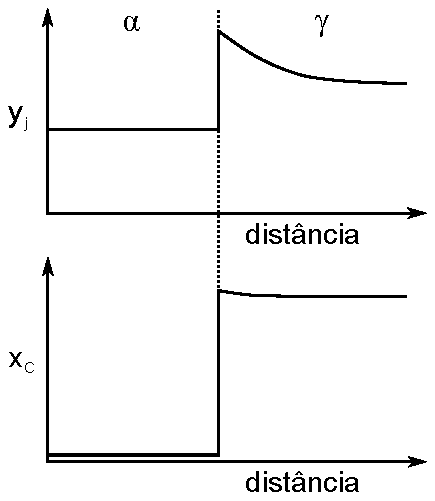
\includegraphics[height=5.8cm]{img/EL-P.pdf}}
  \hspace{1.5cm}
  \subfloat[]{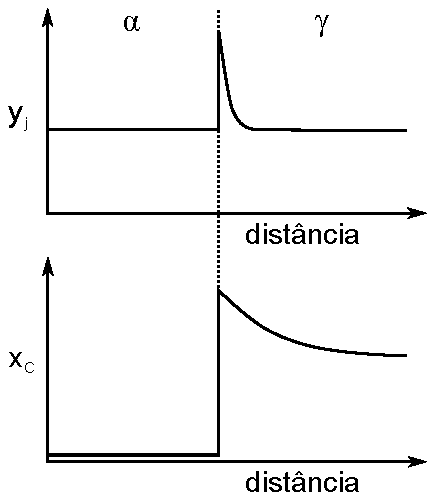
\includegraphics[height=5.8cm]{img/EL-PD.pdf}}
  \vspace{0pt}
  \subfloat[]{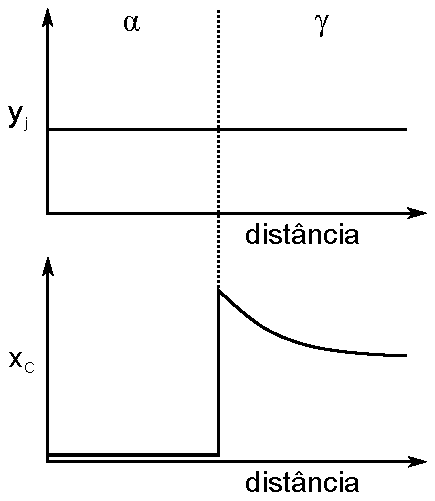
\includegraphics[height=5.8cm]{img/PE.pdf}}
  \caption{Perfis de composição ($x_C$) e fração de sítios ($y_j$) na ferrita ($\alpha$) e na austenita ($\gamma$) segundo os modelos cinéticos de (a) equilíbrio local com partição de soluto (EL-P); (b) equilíbrio local com partição desprezível de soluto (EL-PD); e (c) paraequilíbrio (PE).}
  \label{fig:modcineticos}
\end{figure}

\subsection{Paraequilíbrio (PE)}

\novasigla{PE}{Paraequilíbrio}

\citaremsentenca{Hultgren1947} observou que, durante a decomposição eutetóide da austenita em ferrita e cementita, o produto formado usualmente herdava a mesma composição de elementos substitucionais da fase matriz. Ele chamou estes produtos de paraferrita e paracementita, em oposição às fases de equilíbrio pleno. Em adição, Hultgren argumentou que o crescimento destas \enfase{parafases} ocorreria segundo uma condição termodinâmica específica, denominada paraequilíbrio, na qual duas fases estariam em equilíbrio real uma em relação à outra apenas com respeito aos componentes de maior mobilidade, ou seja, os elementos intersticiais.

A situação de paraequilíbrio ocorre devido à grande diferença de mobilidade entre os solutos substitucionais e o soluto intersticial. Esta situação é passível de ocorrer em baixas temperaturas, quando a difusão dos substitucionais é lenta\cite{Hillert2006}. Adicionalmente, se os elementos substitucionais são impedidos de se redistribuir, seus potenciais químicos individuais não podem ser igualados. Dessa maneira, o comportamento termodinâmico do sistema deve ser avaliado pelo potencial químico $\mu_Z$ do elemento hipotético $Z$\cite{Ghosh2001}, de modo a serem obedecidas as relações termodinâmicas que regem o paraequilíbrio:

\begin{subequations}
  \begin{align}
    \mu_C^\alpha &= \mu_C^\gamma \label{eq:potQuimC}\\
    y_j^\alpha &= y_j^\gamma \label{eq:fracSitios}\\
    \mu_Z^\alpha &= \mu_Z^\gamma \label{eq:potQuimZ}
  \end{align}
\end{subequations}
%
em que $y_j$ são as frações de sítios do elemento $j$ (Mn, Si, Cr, Ni, etc.) nas fases matriz $\gamma$ e em crescimento $\alpha$. Note-se que o potencial químico do elemento teórico $Z$ é definido como a soma dos potenciais químicos dos elementos substitucionais ponderados pelas suas respectivas frações de sítios na fase, isto é:

\begin{equation}
  \mu_Z^p = \sum y_j^p \mu_j^p
\end{equation}

Por sua vez, para um sistema que contém tanto elementos substitucionais, quanto um elemento intersticial (no caso, o carbono), $y_j$ se correlaciona com a fração molar $x_j$ do substitucional na fase pela expressão:

\begin{equation}
  y_j = \frac{x_j}{1 - x_C}
\end{equation}
%
em que $x_C$ é a fração molar do carbono na fase.

A Figura \ref{fig:modcineticos}c ilustra esquematicamente os perfis de composição no crescimento da ferrita a partir da austenita obedecendo as condições de paraequilíbrio. É importante ressaltar que, segundo a definição de Hultgren, tanto as fases formadas segundo o mecanismo de paraquilíbrio, quanto pelo mecanismo de equilíbrio local com partição desprezível de soluto são consideradas parafases. Na situação de EL-PD, embora as composições na interface obedeçam o equilíbrio pleno local, os teores médios de substitucionais em cada fase são praticamente os mesmos\cite{Hillert2004a}.


\section{Transformação martensítica}

\label{sec:Martensita}

Nas ligas ferrosas contendo carbono, quando a decomposição eutetóide da austenita, controlada pela difusão dos elementos de liga, é evitada pelo rápido resfriamento do material a partir da temperatura de autenitização, a austenita tende a se decompor por um mecanismo não difusional na fase metáestável martensita. Nestas ligas a transformação martensítica normalmente gera uma fase de estrutura cristalina tetragonal de corpo centrado em temperaturas inferiores à temperatura de início da transformação martensítica (temperatura Ms). Em situações especiais é possível que uma martensita de estrutura hexagonal compacta se forme a partir da austenita. Outros sistemas de ligas também apresentam transformação do tipo martensítica, mas a importância tecnológica da martensita de ligas baseadas no elemento ferro supera todas as aplicações dos demais sistemas.


A transformação martensítica em aços carbono é acompanhada de expansão volumétrica do material, tal qual ocorre na formação da ferrita a partir da austenita. Como não há redistribuição de soluto entre as duas fases, o produto resultante herda a composição química da fase ancestral de austenita. A presença dos elementos químicos em solução sólida na martensita, em especial o carbono, desempenha papel crítico em seu endurecimento. A formação da martensita é acompanhada da ocupação de posições assimétricas nos sítios intersticiais octaédricos pelos átomos de carbono, fenômeno que leva ao estabelecimento da tetragonalidade da martensita\cite{Zener1946,Hillert1986}. Adicionalmente, a cristalografia da transformação martensítica requer que uma deformação cisalhante seja aplicada à célula unitária da austenita, como teorizado por Bain\cite{Bain1924}. Para compensar este cisalhamento, de modo que um plano invariante macroscópico seja mantido entre as duas fases, é necessário que a martensita recém formada sofra uma distorção para ser acomodada na austenita; essa distorção é conhecida como deformação com plano invariante\cite{Honeycombe2006}. Como ilustrado na Figura \ref{fig:cisMartensita}, essa deformação pode ser obtida por meio do escorregamento de planos cristalinos e consequente criação de discordâncias no interior da fase, ou pela criação de defeitos de maclas na martensita.

\begin{figure}
  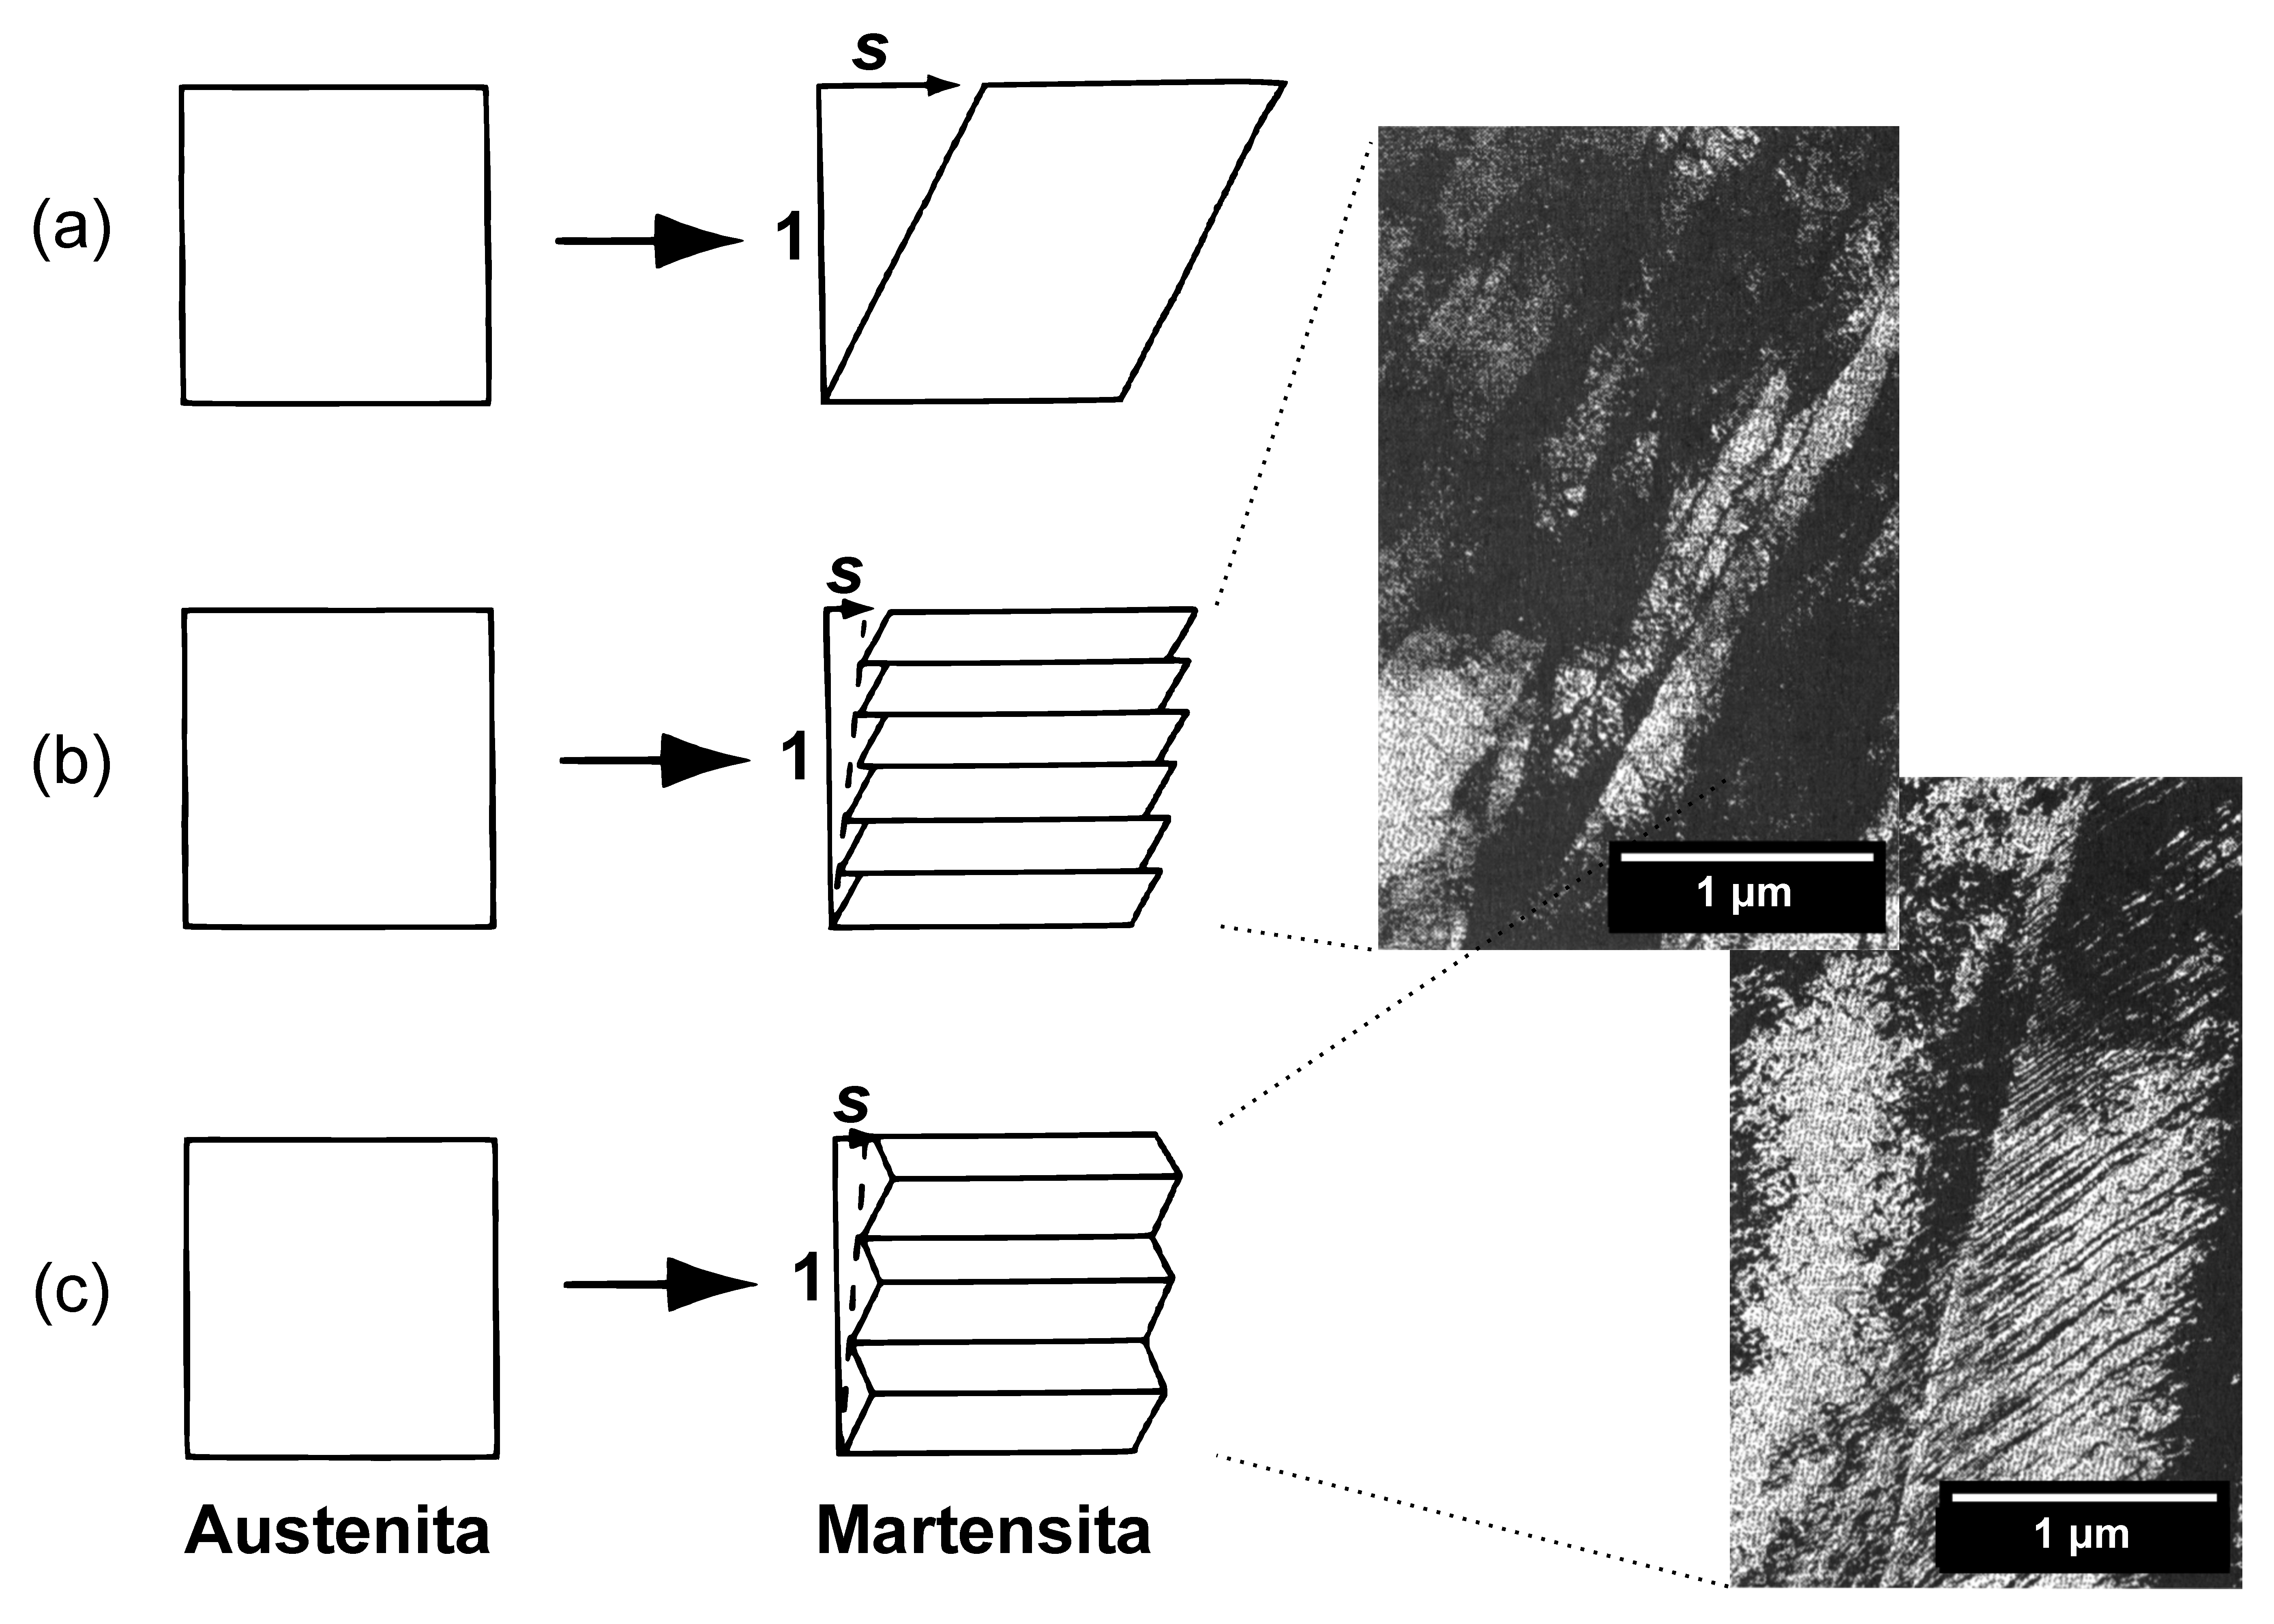
\includegraphics[width=14cm]{img/shearMartensite.pdf}
  \caption{Figura ilustrando que tanto (b) escorregamento quanto (c) maclação podem compensar o cisalhamento \textit{s} produzido pela deformação de Bain esquematizada em (a). No detalhe, imagens obtidas por microscopia eletrônica de transmissão das microestruturas dos dois tipos de martensita. Adaptado de\cite{Porter2009}.}
  \label{fig:cisMartensita}
\end{figure}

A tetragonalidade da martensita aumenta com o aumento da ocupação dos sítios intersticiais pelo carbono. Consequentemente, os defeitos cristalinos relacionados à deformação de plano invariante são mais extensos em ligas de alto carbono. Esse raciocínio leva à conclusão de que a martensita de médio e alto carbono possui elevada dureza, associada, porém, a valores muito baixos de alongamento. Por outro lado, a martensita formada em ligas de baixo carbono pode apresentar estrutura cristalina cúbica de corpo centrado após um certo período de envelhecimento. \citaremsentenca{Speich1972} pontuaram que este fenômeno se deve à segregação do carbono para discordâncias e contornos de ripas de martensita, sendo que o ponto de saturação dos defeitos cristalino ocorre em torno de 0,2\%C.

A natureza da deformação de plano invariante é utilizada para classificação da morfologia da martensita. Assim, a martensita acomodada pela formação de discordâncias e acionamento de planos de escorregamento é denominada martensita escorregada ou, em virtude de sua morfologia característica, martensita em ripas. Por sua vez, a martensita constituída de maclas é chamada de martensita maclada ou em placas. A predominância da ocorrência de uma morfologia ou outra está normalmente associada à composição química da austenita antecessora. Como mostra a Figura \ref{fig:MsZhaoNotis}, dada uma composição fixa, a cada morfologia de martensita é associada uma temperatura Ms. O aumento do teor de carbono leva à diminuição simultânea das duas temperaturas Ms, mas esta tendência é maior para a martensita em ripas. Assim, teores de carbono mais elevados favorecem a formação de martensita em placas, enquanto para aços pouco ligados a martensita em ripas predomina. Por sua vez, a têmpera em aços com teores de carbono intermediários gera microestruturas mistas.

\begin{figure}
  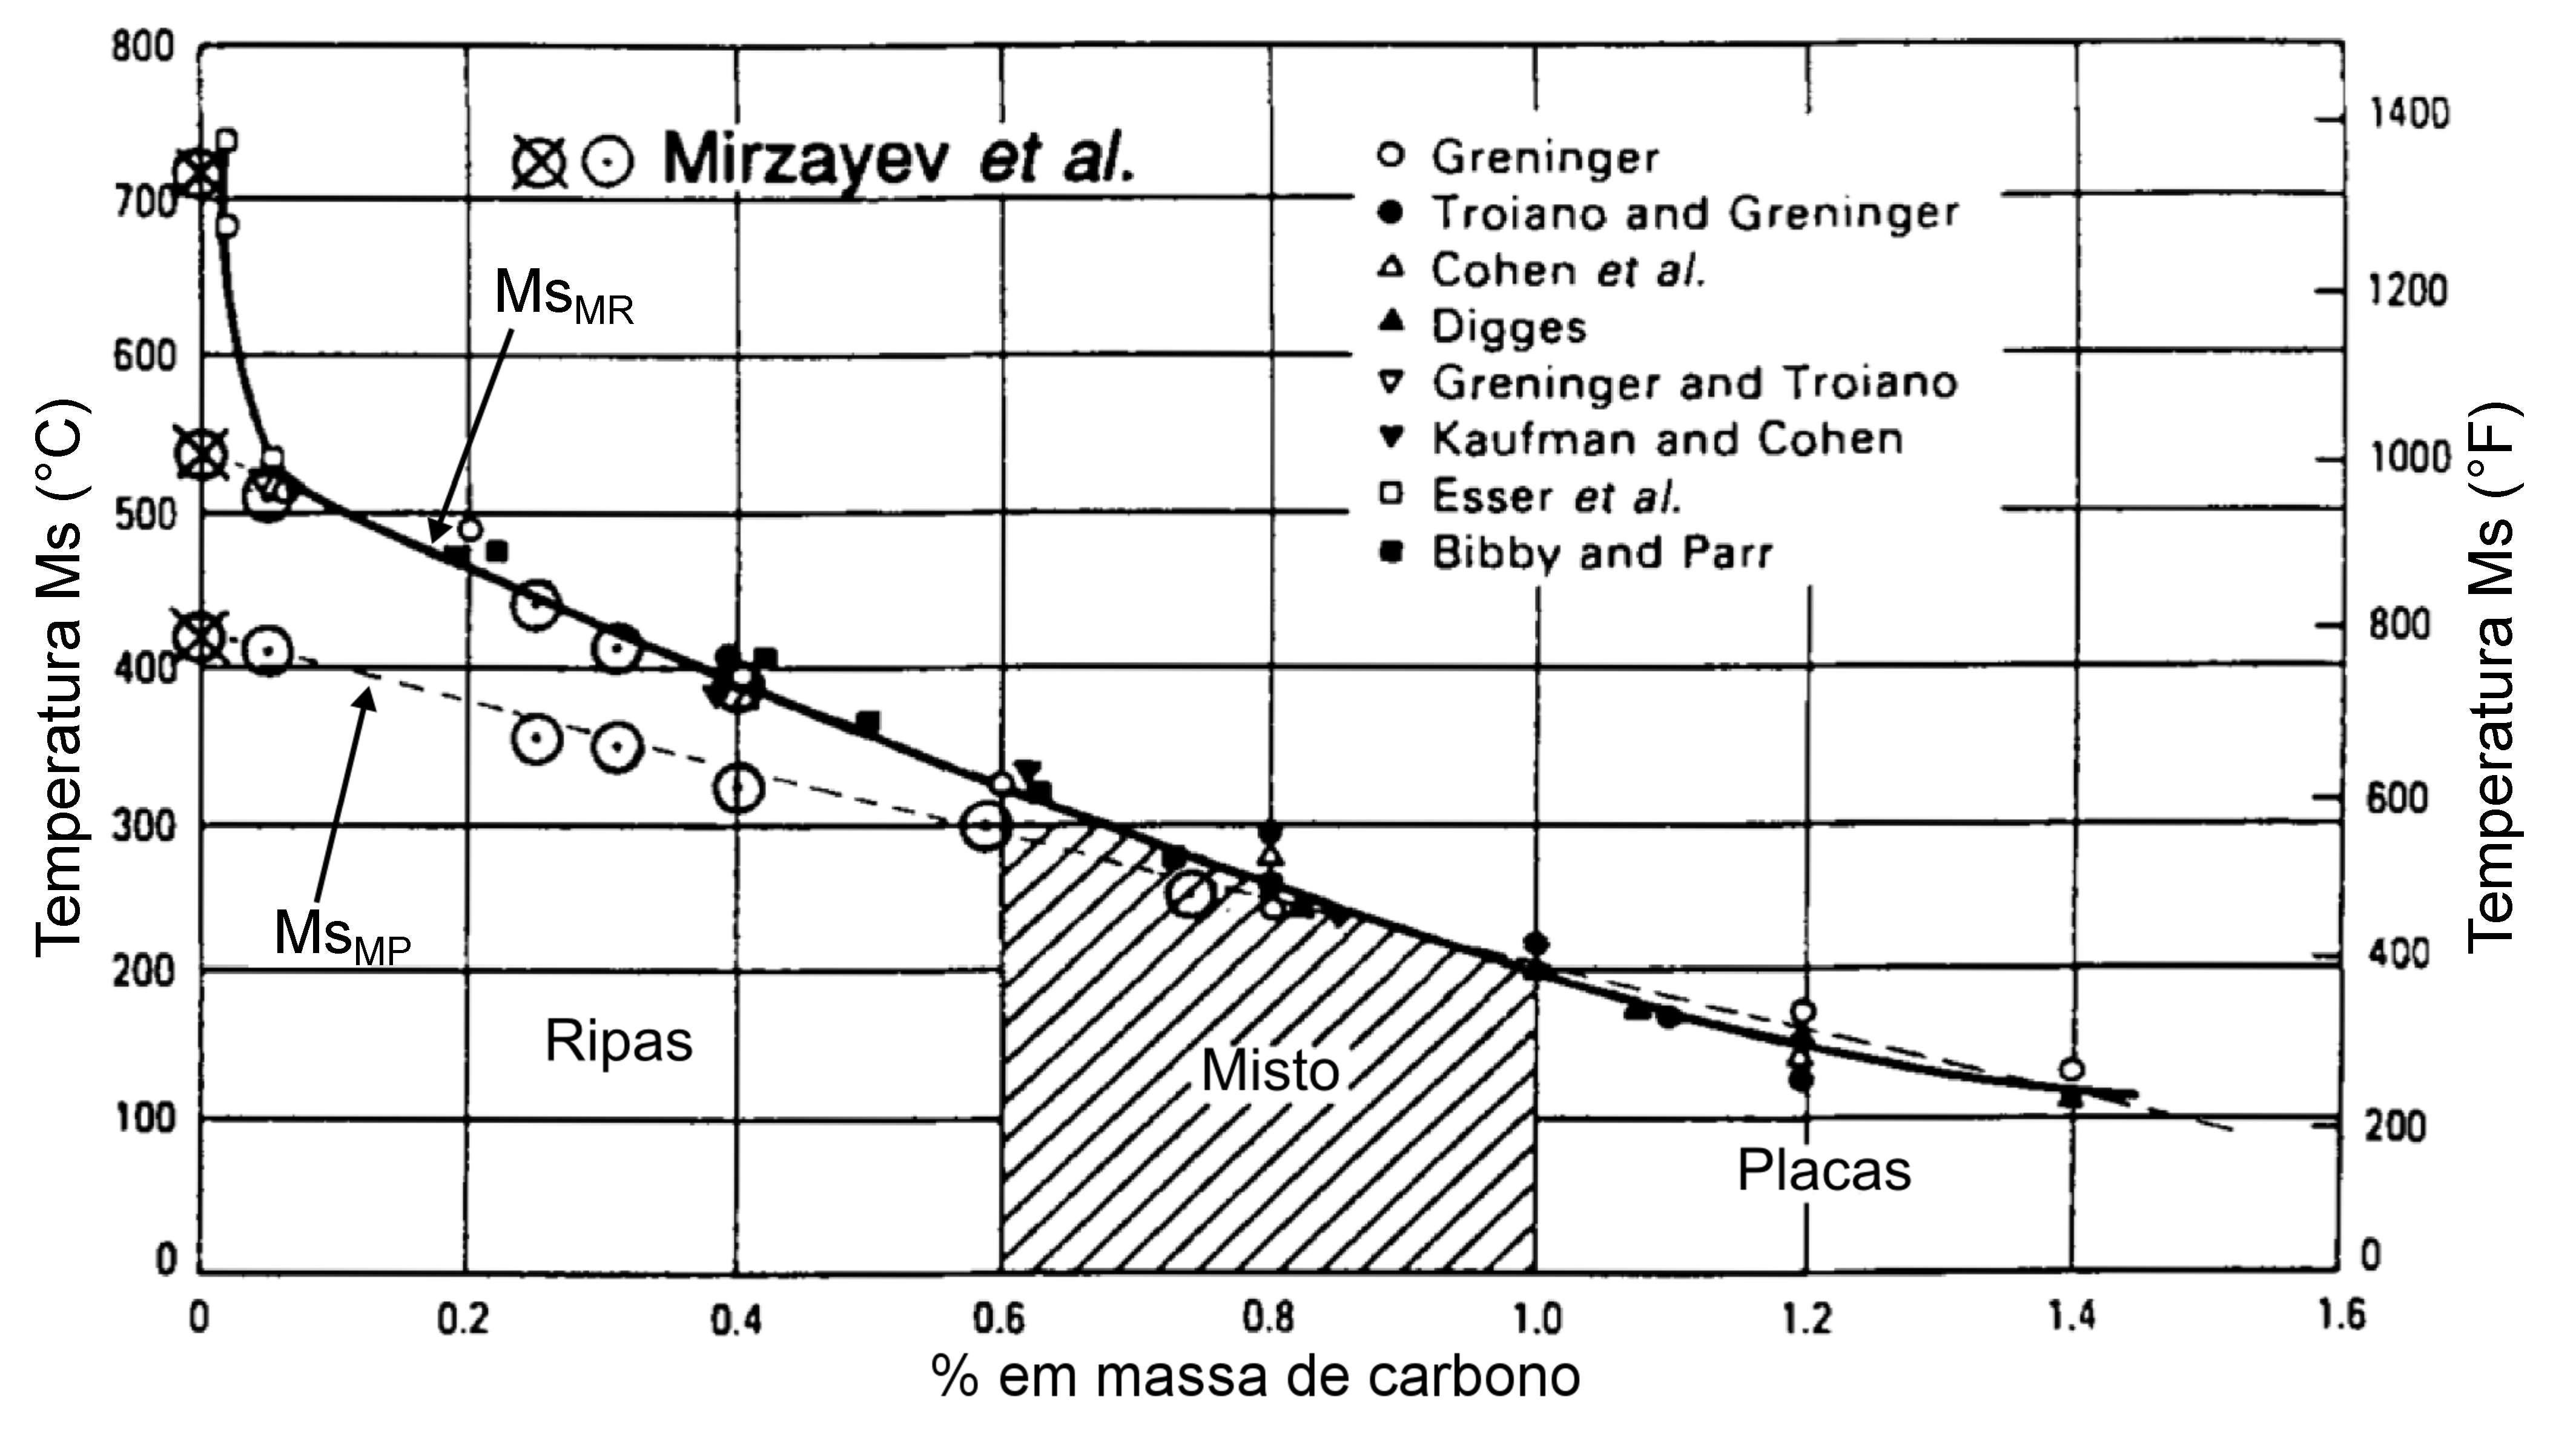
\includegraphics[width=16cm]{img/Ms_Zhao.pdf}
  \caption{Variação das temperaturas início de formação da martensita escorregada ou em ripas ($Ms_{MR}$) e martensita maclada ou em placas ($Ms_{MP}$) em função da composição de ligas Fe-C. Adaptado de\cite{Zhao1995}.}
  \label{fig:MsZhaoNotis}
\end{figure}

Outros elementos de liga também são conhecidos por desempenhar a diminuição da temperatura Ms. De fato, dentre os mais comuns elementos de liga empregados na elaboração de  aços e ferros fundidos, apenas o cobalto é conhecido por elevar a temperatura Ms\cite{Honeycombe2006}. Várias equações empíricas reportadas na literatura foram desenvolvidas para quantificar o efeito dos elementos de liga nesse parâmetro. A mais utilizada é provavelmente a equação de \citaremsentenca{Andrews1965}:

\begin{equation}
  \text{Ms (\SI{}{\degreeCelsius})} = 539 - 423\%w_C^\gamma - \SI{30.4}{}\%w_{Mn}^\gamma - \SI{17.7}{}\%w_{Ni}^\gamma - \SI{12.1}{}\%w_{Cr}^\gamma - \SI{7.5}{}\%w_{Mo}^\gamma
  \label{eq:Andrews}
\end{equation}
%
em que $\%w_i^\gamma$ é a porcentagem em massa do elemento $i$ (C, Mn, Ni, Cr, Mo) dissolvido na austenita. É notável que o efeito do carbono é consideravelmente mais pronunciado do que o dos demais elementos químicos.

A equação de Andrews vale para uma faixa limitada de composições, em geral prevendo razoavelmente bem a temperatura Ms para baixos teores de elementos de liga. Para aços muito ligados, termos de ordem quadrática costumam a pesar na contabilização do efeito do elemento, distanciando a estimativa dos valores experimentais. Além disso, a equação não contabiliza o efeito de alguns importantes elementos de liga empregados na siderurgia moderna, como microligantes (e.g., Ti, Nb, V) e elementos utilizados para supressão da precipitação de carbonetos (Si e Al). Uma compilação das equações empíricas disponíveis na literatura para o cálculo do Ms é disponível no trabalho de \citaremsentenca{Liu2001}, sendo reforçado pelos autores que as equações são somente válidas para aços de baixa liga.

Outro aspecto importante do entendimento da transformação martensítica é a determinação da fração transformada em função da temperatura de reação. Como a transformação martensítica ocorre sem difusão, dada uma taxa de resfriamento fixa, a fração transformada de martensita deve depender apenas do super-resfriamento abaixo da temperatura Ms, e não do tempo de permanência na temperatura de têmpera $T_T$, como expresso na equação empírica de Koistinen-Marburger\cite{Koistinen1959}:

\begin{equation}
  f^{\alpha'} = 1 - f^\gamma = 1 - \exp \left[ - \beta \left( Ms' - T_T \right)\right]
  \label{eq:KM}
\end{equation}
%
em que $f^{\alpha'}$ e $f^\gamma$ são, respectivamente, a fração transformada de martensita e a fração não-transformada de austenita e $\beta$ e Ms' são ambos coeficientes de ajuste. $\beta$ é associado à taxa de transformação, cujo valor determinado originalmente por Koistinen e Marburger é de \SI{1.1e-2}{\degreeCelsius^{-1}}, válido para várias ligas. Entretanto, este parâmetro pode sofrer variações de acordo com a composição e parâmetros de tratamento térmico do material. Por sua vez, Ms' corresponde à temperatura em que $f^{\alpha'} = 0$, isto é, em teoria trata-se da temperatura Ms de início da transformação martensítica. No entanto, o valor de Ms' é frequentemente inferior à real temperatura Ms da liga. Isso ocorre porque para pequenos super-resfriamentos a curva de transformação martensítica é lenta e não é bem descrita pela equação de Koistinen-Marburger. Tanto $\beta$ quanto $Ms'$ podem ser determinados a partir do ajuste da curva de transformação martensítica determinada experimentalmente pela equação \ref{eq:KM}. A determinação experimental da curva de transformação é comumente feita por meio de métodos de medidas de cinética global, como experimentos de dilatometria e resistividade elétrica\cite{DeMoor2009}.


Um fato previsto pela equação de Koistinen-Marburger é que ligas com baixas temperaturas Ms devem reter grandes quantidades de austenita não-transformada na temperatura ambiente. Assim, tendo em vista a interpretação da equação de Andrews (equação \ref{eq:Andrews}), quanto maior o teor de elementos de liga na austenita (salvo o caso do cobalto), maior sua capacidade de ser retida na temperatura ambiente.

É importante ser ressaltado que a generalização sobre a atuação dos elementos de liga no controle da proporção das fases após a têmpera só é possível porque a mistura martensita + austenita está distante do equilíbrio termodinâmico. \citaremsentenca{Honeycombe2006} classificam elementos de liga nos aços em duas categorias: alfagênicos e gamagênicos, ou seja, estabilizadores da ferrita (fase $\alpha$) ou da austenita (fase $\gamma$). Nesta distinção, os elementos são classificados de acordo com sua capacidade de ampliar ou contrair o campo austenítico do ferro em temperaturas elevadas, segundo o diagrama de equilíbrio. Esse argumento leva, por exemplo, a afirmações aparentemente contraditórias, mas verídicas, como o fato do elemento cromo contrair o campo austenítico, mas, quando em solução sólida na austenita, favorecer a retenção da austenita após a têmpera do material.

Neste texto, o conceito de estabilidade da austenita foi adotado em um sentido menos rigoroso, denotando a capacidade da fase manter suas propriedades após sua exposição a solicitação mecânica e condições cinéticas (tempo e temperatura) favoráveis para sua decomposição.

%efeito TRIP é abordado na seção \ref{subsec:TRIP}. Transfomação isotérmica da martensita são abordados na seção \ref{subsec:decompMs}

\subsection{Estabilidade mecânica da austenita e efeito TRIP}

\label{subsec:TRIP}

Ainda que a austenita seja retida à temperatura ambiente, em decorrência de sua metaestabilidade termodinâmica, caso seja fornecida alguma espécie de ativação ao material esta fase pode se decompor em produtos que reduzem a energia livre do sistema. O efeito TRIP (\enfase{Transformation-induced plasticity}) acontece quando a austenita é submetida a um trabalho de deformação plástica e se transforma em martensita. A transformação martensítica induzida por tensões locais tem o efeito de aliviar a concentração de tensões, aumentando a taxa de encruamento e promovendo deformação homogênea, com consequentes melhorias na resistência, ductilidade e tenacidade do material\cite{Honeycombe2006}.

\novasiglaestrangeira{TRIP}{Transformation-induced plasticity}

Em aços inoxidáveis austeníticos este fenômeno é bem conhecido. %pegar ou o trabalho do Wasserman, ou o trabalho do Zackay. vide\cite{DeCooman2004}
Nestas ligas, a deformação plástica leva primeiramente à formação de martensita hexagonal nucleada nas falhas de defeito de empilhamento (maclas), sendo subsequentemente transformada em martensita tetragonal\cite{Honeycombe2006}. O efeito TRIP, no entanto, só ocorre quando a deformação é aplicada em temperaturas abaixo de uma temperatura Md característica da fase. Quanto maior a temperatura, maior a energia de defeito de empilhamento (EDE) da austenita e, portanto, menor é a força motriz para a transformação ocorrer. A temperatura Md define termodinamicamente o ponto em que o trabalho de deformação aplicado ao material é compensado pelo aumento da EDE\cite{DeCooman2004} e a força motriz para transformação é nula. Alternativamente, a temperatura Md é entendida como a maior temperatura em que é termodinamicamente possível que a transformação martensítica ocorra pela deformação da austenita.


A temperatura Md pode ser utilizada como um parâmetro para se verificar se o fenômeno TRIP trará os benefícios mencionados acima. Não é desejável que a temperatura Md seja maior do que a temperatura de utilização do material, de modo que o fenômeno TRIP não ocorra. Por outro lado, caso a austenita se deforme sob aplicação de tensões/deformações muito pequenas, o material também não terá melhoria em ductilidade. Reporta-se na literatura que há uma quantidade ótima de carbono na austenita retida que aumenta o alongamento; valores muito baixos ou muito altos não produzem melhoria do alongamento\cite{Reisner1997,Meyer1999}.

Além disso, o condicionamento da microestrutura também afeta a estabilidade mecânica da austenita. Tamanho, morfologia e distribuição da austenita na microestrutura são variáveis que definem o comportamento mecânico desta fase\cite{Timokhina2004}. Grãos menores de austenita contêm menos sítios potenciais para nucleação de martensita. Assim, regiões que contêm grãos grosseiros e/ou blocos isolados de austenita tendem a ser mais instáveis e transformam-se facilmente, contribuindo pouco para o aumento da ductilidade. Por outro lado, grãos submicrométricos de austenita possuem menor tendência de se transformar e a austenita acaba sofrendo intenso encruamento, contribuindo pouco com o efeito TRIP\cite{Bai1998}. Por sua vez, materiais que apresentam austenita na forma de filmes entre subunidades de bainita isenta de carbonetos e entre ripas de martensita apresentam melhor comportamento em relação ao alongamento\cite{Takahashi1991,Xiong2013}.

Ligas modernas são produzidas com quantidades controladas de austenita estabilizada para se beneficiar do efeito TRIP. Um exemplo destes aços multifásicos que já tem atingido alto volume de aplicações são chapas de aços TRIP (\enfase{TRIP-assisted steels}) para aplicações na indústria automotiva. Estes aços contém uma estrutura de ferrita equiaxial produzida pela austenitização parcial no campo intercrítico e bainita isenta de carbonetos entremeada com austenita retida, produzida por um tratamento de austêmpera. Assim como nos ADIs, o projeto de liga destes aços contém teores controlados de silício, alumínio ou fósforo para evitar a precipitação de carbonetos durante a reação bainítica, permitindo a partição de carbono para estabilizar a austenita não transformada\cite{DeCooman2004,Honeycombe2006}.

O processo de Têmpera e Partição também tem como objetivo a produção de microestruturas multifásicas contendo austenita retida estabilizada à temperatura ambiente. Este tópico é abordado na próxima seção do texto.

\section{O processo de Têmpera e Partição (T\&P)}

\label{sec:processoTP}
 
O caráter frágil da martensita como temperada exige que tratamentos térmicos subsequentes sejam aplicados ao material para que exigências de tenacidade sejam obedecidas. O tratamento de revenimento consiste do tratamento isotérmico da martensita em temperaturas na faixa de 150 a \SI{700}{\degreeCelsius}. O propósito do revenimento é fornecer ativação térmica ao material para que a microestrutura se aproxime do estado de equilíbrio, promovendo a decomposição da austenita não-transformada (retida) e o alívio da supersaturação de carbono da martensita para formação de microestruturas que minimizam a energia livre do sistema\cite{Honeycombe2006}. As microestruturas da martensita revenida dependem da temperatura de revenimento, mas na comumente consistem de uma mistura de carbonetos e de martensita empobrecida em carbono.

A redistribuição do carbono da martensita para a austenita durante o revenimento é um fato conhecido a longa data\cite{Matas1960}. No entanto, sobretudo devido à formação de carbonetos desde as etapas iniciais do revenimento, até recentemente este fato nunca fora aproveitado para o desenvolvimento de microestruturas de interesse tecnológico. Em 2003, \citaremsentenca{Speer2003} afirmaram que quando a precipitação de carbonetos é suprimida, a \enfase{partição} do carbono da martensita para austenita poderia ser conseguida mesmo a altas temperaturas. Neste trabalho os autores apresentaram um modelo termodinâmico para determinar o teor de carbono na austenita e predição da microestrutura após a partição de carbono. Baseado nestes conceitos de controle da fração transformada de martensita e de estabilização da austenita pelo seu enriquecimento de carbono, os autores sugeriram uma nova rota de tratamento térmico denominada \sigla{T\&P}{Têmpera e Partição}.

O processo T\&P é esquematizado na Figura \ref{fig:esqTP}. Após a austenitização total ou parcial da liga, o material é temperado até uma temperatura de têmpera $T_T$ abaixo da temperatura Ms para produzir uma mistura controlada de martensita e austenita. Em seguida, na etapa de partição, o material é mantido em um patamar isotérmico em uma temperatura de partição $T_P$ igual ou superior a $T_T$ para permitir a partição de carbono da martensita para a austenita. Como mencionado anteriormente, o carbono em solução sólida diminui a temperatura Ms da austenita, eventualmente para temperaturas inferiores à ambiente, estabilizando-a à temperatura ambiente. A viabilidade do processo T\&P depende da supressão da precipitação de carbonetos durante a etapa de partição, que consumiriam parte do carbono que outrora seria particionado para a austenita. Para tanto, são empregados elementos de liga que retardam essas reações, como os já citados silício, alumínio e fósforo.

\begin{figure}
  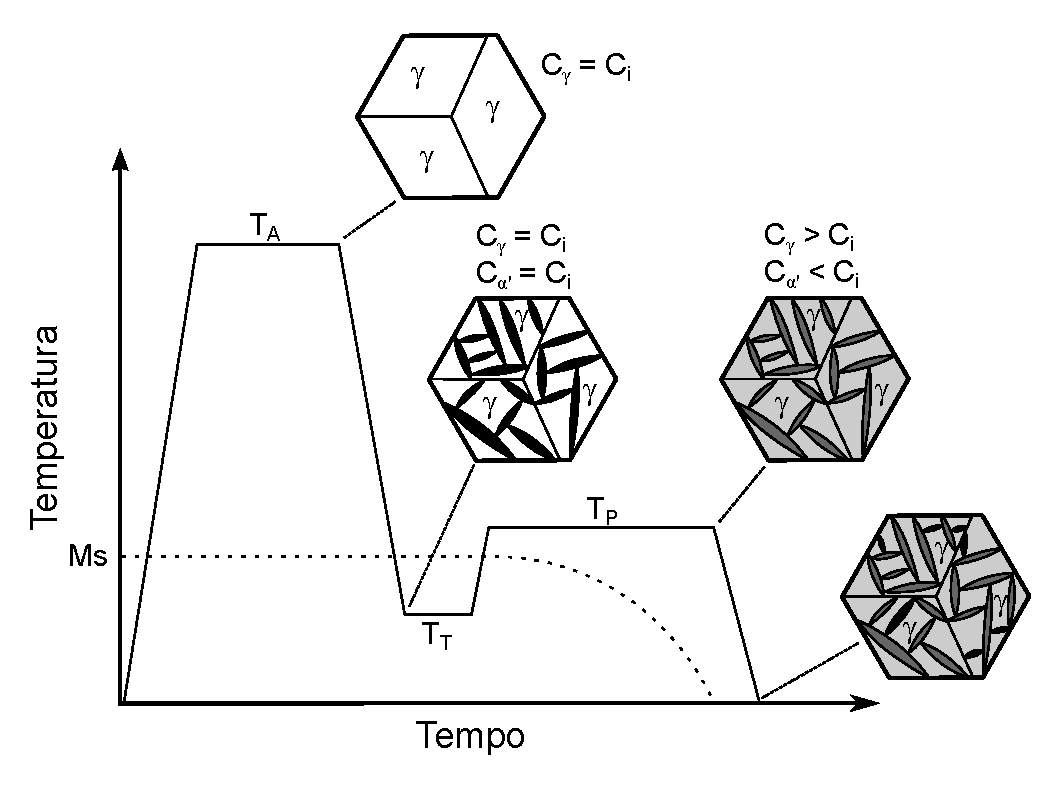
\includegraphics[height=9cm]{img/esquemaTP.pdf}
  \caption{Figura esquemática do tratamento de Têmpera e Partição (T\&P). $T_A$, $T_T$ e $T_P$ representam as temperaturas de austenitização, de têmpera e do tratamento de partição, enquanto $C_{i}$, $C_{\gamma}$ e $C_{\alpha\text{'}}$ representam as concentrações de carbono inicial, da austentita e da martensita, respectivamente. Adaptado da referência\cite{Edmonds2006}. }
  \label{fig:esqTP}
\end{figure}

Uma vez que permite controlar de uma forma relativamente fácil a microestrutura do material, o processo T\&P é capaz de produzir a partir de uma mesma formulação de liga, materiais com diferentes comportamentos mecânicos. A martensita particionada confere resistência mecânica semelhante àquela obtida durante o tratamento de revenimento, enquanto a austenita confere ductilidade e tenacidade em decorrência do fenômeno TRIP\cite{Matlock2010}. Por estes motivos, materiais temperados e particionadas tem sido produzidos no desenvolvimento de chapas de aços de alta resistência, atingindo combinações de propriedades correspondentes a uma classe inteiramente nova de aços.

\citaremsentenca{Matlock2003} conduziram uma investigação inicial do conceito T\&P em barras de aços médio carbono (0,35\% em massa) microligado. Os autores verificaram grande quantidade de austenita retida enriquecida em carbono no produto final, embora aparente formação de carbonetos de transição não fora evitada durante a etapa de partição. Gendermann apud\cite{Speer2004} examinou as propriedades mecânicas de aço AISI 9260 modificado com adição de teores elevados de Si (2\% em massa) submetido ao processo T\&P, avaliando as variáveis temperatura de têmpera e tempo e temperatura de partição. Quantidades de austenita próximas a 30\% em volume foram obtidos para amostras temperadas a \SI{190}{\degreeCelsius} e particionadas a \SI{500}{\degreeCelsius} por 10 segundos. Quantidades significativas de austenita retida não foram obtidas quando o material foi temperado e revenido, enquanto menores valores de dureza foram obtidos para o material austemperado.

\novasiglaestrangeira{AISI}{American Iron and Steel Institute}

Como mencionado na seção \ref{subsec:TRIP}, aços TRIP contém quantidades significativas de austenita estabilizada, esta produzida pela interrupção da reação bainítica durante a estase, e também fazem uso de elementos de liga para suprimir a precipitação de carbonetos. Dessa forma, é natural que ligas semelhantes às utilizadas nestes aços sejam submetidas ao processo de Têmpera e Partição. \citaremsentenca{Streicher2004} %Arranjar futuramente o documento desse artigo http://digital.library.aist.org/pages/PR-255-006.htm
avaliaram os aspectos de transformações de fases e a resposta a solicitações mecânicas de um aço ligado ao silício (1,63\% em massa) submetido ao processo T\&P. Variações do processamento envolveram a realização do tratamento térmico em uma ou duas etapas. As combinações de propriedades dos materiais temperados e particionados forneceram valores semelhantes de resistência à tração associados a valores de alongamento mais elevados do que a classe de aços martensíticos. Estes resultados, comparados a outras classes de aços modernos, são mostrados na Figura \ref{fig:TRIPQP}.

\begin{figure}
  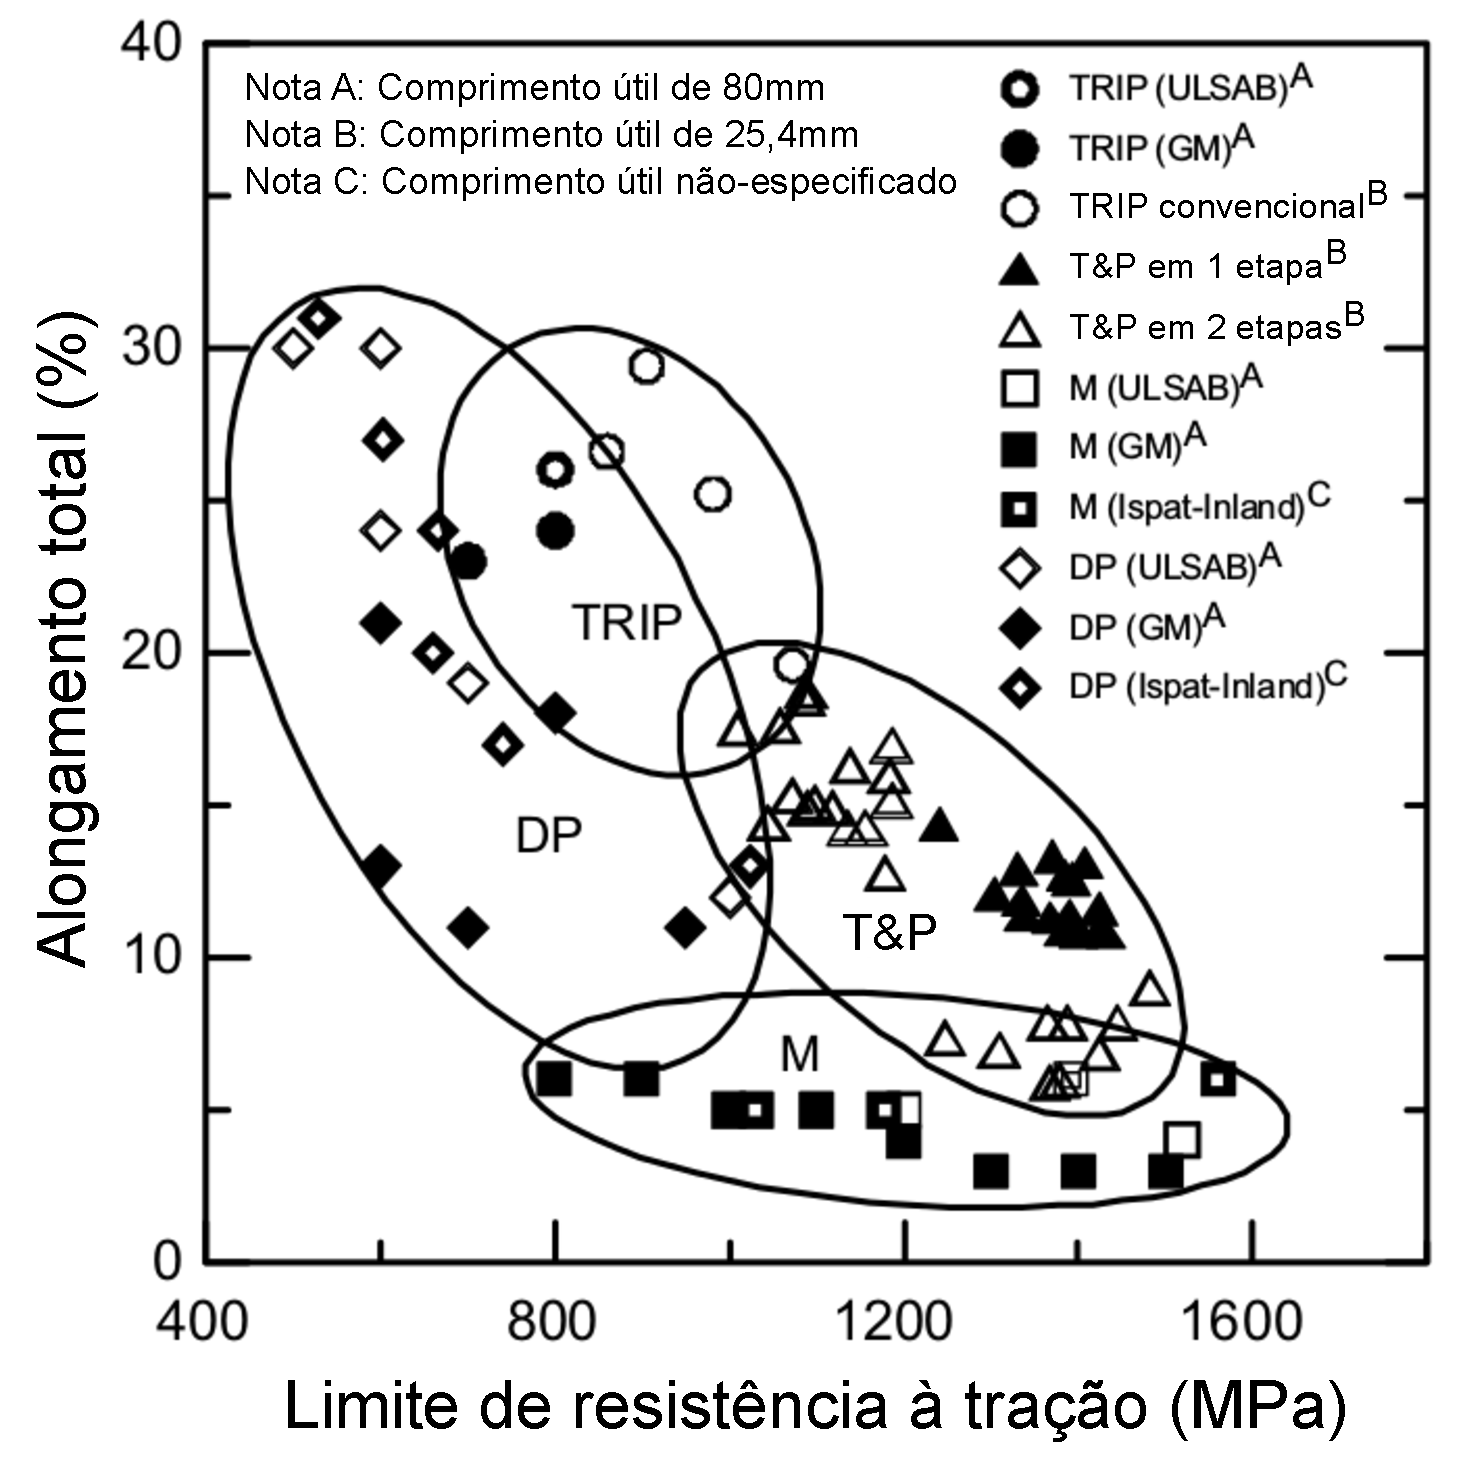
\includegraphics[height=10cm]{img/Streicher.pdf}
  \caption{Alongamento total versus limite de resistência à tração agrupados segundo classes de aços TRIP, \textit{Dual Phase} (DP), martensítico (M) e T\&P tratados em uma ou duas etapas\cite{Streicher2004}.}
  \label{fig:TRIPQP}
\end{figure}

Alinhado ao escopo do presente trabalho, um grupo de estudantes de graduação da \enfase{Colorado School of Mines} examinaram a viabilidade do processo de Têmpera e Partição em um ferro fundido nodular, obtendo quantidade substancial de austenita retida enriquecida em carbono e aumento de resistência mecânica em relação ao ferro fundido nodular austemperado. Entretanto, a quantidade de austenita retida foi menor do que a obtida pelo tratamento de austêmpera, implicando em perda de ductilidade. Os autores comentam que os resultados obtidos foram difíceis de interpretar diante das diferenças entre as frações de fase obtidas durante a têmpera, da precipitação de carbonetos e do comportamento das amostras durante a partição, concluindo que experimentação adicional deveria ser realizada para melhor caracterização do fenômeno\cite{Speer2004}.

No grupo de pesquisa em que se insere o presente trabalho, \citaremsentenca{Silva2013} avaliou a microestrutura e o comportamento mecânico de duas ligas comerciais de ferro fundido com alto manganês (> 0,5\%) tratadas pelo processo T\&P. Silva observou extensas regiões de ausferrita na microestrutura dos materiais tratados termicamente e a ocorrência de uma janela de processo, análoga à precipitação de carbonetos no segundo estágio da reação bainítica no ADI. Os materiais produzidos apresentaram propriedades nos limites da especificação da norma ASTM A897 para ferros fundidos austemperados. Em um trabalho recente, \citaremsentenca{Silva2014} discutiram que as propriedades baixas, ainda que dentro das especificações para ADIs, foram consequência da superposição das janelas de processo das regiões de contorno de célula eutética e próximas aos nódulos. Dessa forma, para incremento das propriedades do ferro fundido T\&P, o teor de manganês haveria de ser diminuído e a inoculação aumenta, minimizando os problemas associados à segregação.

\novasiglaestrangeira{ASTM}{ASTM International}
%"O leitor verá que em algumas partes do texto a martensita de baixo carbono é referenciada como ferrita e vice-versa"

\subsection{Termodinâmica da partição de carbono no processo T\&P}

Para compreender as condições termodinâmicas que definem o equilíbrio após o tratamento T\&P, \citaremsentenca{Speer2003} inicialmente assumiram que a redistribuição de carbono entre martensita e austenita ocorreria sem a movimentação da interface. Adicionalmente, como a martensita herda a composição da austenita após a têmpera, a martensita particionada, resultante da relaxação do carbono, deve manter a mesma razão de elementos substitucionais que a austenita. Segundo a definição de Hultgren, portanto, a martensita particionada trata-se essencialmente de paraferrita.

Inicialmente esta condição foi chamada de \enfase{Constrained Paraequilibrium}, ou \sigla{PER}{Paraequilíbrio Restringido}, dada a semelhança com as ideias de Hultgren, com o adendo de que é imposta uma restrição de que os átomos de ferro e substitucionais permanecem completamente imóveis durante a partição de carbono. Dessa forma, a condição proposta prevê que a fração de sítios dos elementos substitucionais permanece equivalente na austenita e na martensita (equação \ref{eq:potQuimC}) e que a igualdade entre os potenciais químicos de carbono na martensita e na austenita também é obedecida (equação \ref{eq:fracSitios}). Entretanto, em troca da imposição de que interface martensita/austenita deve permanecer imóvel, a condição de igualdade dos potenciais químicos do elemento hipotético $Z$, representada pela equação \ref{eq:potQuimZ}, não pode mais ser mantida. Assim, a condição de metaestabilidade é atingida pela minimização da energia livre, dadas as restrições estabelecidas.

Em trabalhos recentes, a condição de paraequilíbrio restringido tem sido referenciada por \enfase{Constrained Carbon Equilibrium}, ou \sigla{ERC}{Equilíbrio Restringido de Carbono}, após discussão realizada entre Speer e colaboradores e Hillert e {\AA}gren\cite{Hillert2004a,Speer2005e,Hillert2005}. \citaremsentenca{Hillert2004a} argumentaram que a relação entre paraequilíbrio e a definição de paraequilíbrio restringido seria mínima, pois: a) paraequilíbrio já se trata de um equilíbrio restringido; b) paraequilíbrio se refere a condições em que ocorre movimentação de interface; c) a redistribuição de elementos substitucionais próximo à interface é praticamente inevitável; d) devido ao requerimento de minimização de energia livre, o PER seria apenas aplicável para o estado final, enquanto a condição de paraequilíbrio se aplica para o crescimento de uma nova fase; e) a redistribuição dos elementos substitucionais para a interface martensita/austenita teria efeito desprezível na redistribuição do carbono entre as duas fases, já que esta é controlada pelas atividades do carbono. O resultado da equilibração de carbono, portanto, seria independente das condições da interface martensita/austenita.

Em resposta a Hillert e {\AA}gren, \citaremsentenca{Speer2005e} pontuaram que, em essência, o conceito proposto de PER é similar ao de paraequilíbrio, estendido ao ponto de quando a interface permanece imóvel e que não veriam motivo para que houvesse confusão entre as terminologias adotadas. Posteriormente, \citaremsentenca{Hillert2005} reconheceram que a discussão sobre a relação entre paraequilíbrio e PER adquirira características filosóficas e que se tratava, de fato, em aceitar a ampliação do conceito de paraequilíbrio para além de seu campo de aplicação original. Hillert e {\AA}gren assinalaram que seria desejável preservar o conceito original e sugeriram a utilização do termo \enfase{Constrained Carbon Equilibrium}, apresentado anteriormente. Atualmente esta terminologia parece ter adquirido aceitação geral e vem sendo utilizada desde então\cite{Edmonds2006, Speer2007}. 
No Brasil, as recentes teses sobre Têmpera e Partição tem adotado a denominação \enfase{Equilíbrio Constrito de Carbono} (ECC)\cite{Martins2007, Coelho2008}. Neste trabalho, a utilização da tradução alternativa Equilíbrio Restringido de Carbono foi adotada por acreditar-se que a palavra \enfase{restringido} trata-se de uma melhor tradução do inglês de \enfase{constrained} do que \enfase{constrito}.

\subsubsection{Cálculo do ERC para ligas Fe-C}

\label{subsubsec:ERC}

O cálculo do ERC em uma determinada liga ferrosa depende de dois principais parâmetros de entrada: a composição química --- em especial, o teor de carbono da liga --- e a fração inicial de austenita não transformada (ou, alternativamente, a fração de martensita)\cite{Speer2003}. Para uma dada condição de austenitização (plena ou parcial), a fração inicial austenita não transformada $f_i^\gamma$ depende da temperatura da têmpera $T_T$ aplicada ao material e pode ser estimada pela equação de Koistinen-Marburger (equação \ref{eq:KM}), apresentada anteriormente. Além disso, uma vez que a condição de equilíbrio restringido de carbono impõe uma restrição geométrica ao sistema (imobilidade da interface), o cálculo do ERC requer, além de dados termodinâmicos obtidos na literatura ou por simulações termodinâmicas, equações secundárias que caracterizam a conservação dos constituintes na microestrutura.

Lobo e Geiger\cite{Lobo1976a,Lobo1976b} determinaram as atividades para o carbono na ferrita e na austenita no sistema Fe-C em relação ao estado padrão da grafita.
Para este caso simplificado, é possível ilustrar o problema do cálculo do ERC para um aço carbono. É conveniente, neste caso, expressar os dados na seguinte forma simplificada obtida por \citaremsentenca{Bhadeshia1981}:

\begin{equation}
  RT \ln\frac{\Gamma_C^\alpha}{\Gamma_C^\gamma} = 76789 - 43,8T - (169105 - 120,4) x_C^\gamma
  \label{eq:ativC}
\end{equation}
%
em que $\Gamma_C^\alpha$ e $\Gamma_C^\gamma$ são respectivamente os coeficientes de atividade Henriana do carbono na ferrita e na austenita, $x_C^\gamma$ é a fração molar de carbono na austenita, $R$ é a contante universal dos gases, equivalente a aproximadamente \SI{8.314}{J mol^{-1} K{-1}}, e $T$ é a temperatura absoluta.


Como a atividade do carbono na fase é calculada pelo produto do coeficiente de atividade pela fração molar de carbono (i.e., $a_C = \Gamma_C x_C$), a condição que leva à equivalência das atividades e dos potenciais químicos do carbono nas duas fases (equação \ref{eq:potQuimC}) é dada pela equação:

\begin{subequations}
  \begin{align}
    x_C^\alpha = x_C^\gamma \exp \left [ - \frac{76789 - 43,8T - (169105 - 120,4T) x_C^\gamma}{RT} \right ]\label{eq:ativC2}
  \end{align}
\end{subequations}
%
em que $x_C^\alpha$ é a fração molar de carbono na ferrita.

As demais equações constitucionais definem o problema por completo:

\begin{subequations}[resume]
  \begin{align}
    &f_{ERC}^\gamma \left ( 1 - x_{C_{ERC}}^\gamma \right ) = f_i^\gamma \left ( 1 - x_{C_i}^\gamma \right )\label{eq:balSubs}\\
    &f_{ERC}^\alpha x_{C_{ERC}}^\alpha + f_{ERC}^\gamma x_{C_{ERC}}^\gamma = x_{C_i}^\gamma\label{eq:balC}\\
    &f_{ERC}^\alpha + f_{ERC}^\gamma = 1\label{eq:balFases}
  \end{align}
\end{subequations}
%
em que $x_{C_i}^\gamma$ é o teor de carbono inicial da austenita, $x_{C_{ERC}}^\alpha$ e $x_{C_{ERC}}^\gamma$ são os teores de carbono na martensita e na austenita na condição de equilíbrio restringido de carbono e $f_{ERC}^\alpha$ e $f_{ERC}^\gamma$ são as frações molares de martensita particionada e austenita na condição de ERC.

A equação \ref{eq:balSubs} estabelece o balanço de massa dos átomos de substitucionais entre a austenita não-transformada inicial e austenita na condição de ERC. Note-se que a fração molar da austenita varia dependendo do teor de carbono adquirido após a relaxação de carbono. Essa percepção, inicialmente não intuitiva, dada a hipótese de interface imóvel, encontra justificativa no fato de que a fração molar da fase depende também da fração de sítios ocupados pelo carbono. Assim, variações sutis na fração molar da austenita são oriundas da maior ou menor ocupação dos sítios intersticiais por átomos de carbono.

Por sua vez, a equação \ref{eq:balC} denota um balanço de carbono pela soma ponderada dos teores de carbono na martensita e na austenita. A equação \ref{eq:balFases} estabelece a relação entre as frações de fase, que devem somar a unidade no caso de austenitização plena, ou um valor menor do que um, equivalente à fração de austenita obtida após o tratamento de austenitização.

A condição de ERC é representada pela solução simultânea das quatro equações \ref{eq:ativC2}--\ref{eq:balFases} para as quatro variáveis desconhecidas $x_{C_{ERC}}^\alpha$, $x_{C_{ERC}}^\gamma$, $f_{ERC}^\alpha$ e $f_{ERC}^\gamma$. A resolução deste sistema não-linear deve ser feita numericamente, pois não apresenta solução analítica.

A formulação descrita acima é estritamente aplicável ao caso do sistema Fe-C, mas pode ser utilizada com considerável fidelidade para aços de baixa liga\cite{Speer2003}. Para que o método adquira caráter rigoroso para as demais ligas, as equações \ref{eq:ativC} e \ref{eq:ativC2} devem ser modificadas para as atividades do carbono expressas em função dos devidos parâmetros de interação do carbono com os demais elementos de liga. Alternativamente, as atividades do carbono na ferrita e na austenita podem ser determinados utilizando cálculos de termodinâmica computacional.

% \subsubsection{Determinação da temperatura ótima de têmpera}

% \label{subsec:tempOtima}

% O cálculo do ERC para diferentes temperaturas de têmpera permite a determinação dos parâmetros de tratamento térmico que levam a uma maior retenção de austenita estabilizada por carbono no material. Uma simples metodologia desenvolvida por Speer et al. apud\cite{Edmonds2006} faz uso de equações empíricas para determinação da temperatura Ms (tal qual a equação de Andrews) e da equação de Koistinen-Marburger (equação \ref{eq:KM}) para a computação da fração inicial de austenita não transformada ($f_i^\gamma$) em função da temperatura de têmpera $T_T$.

% Tendo como parâmetros de entrada $f_i^\gamma$ e o teor de carbono inicial da austenita $x_{C_i}^\gamma$, o ERC é resolvido para uma temperatura de partição $T_P$. $T_P$ é necessário para o cálculo da relação entre as frações molares de carbono na ferrita e na austenita, expressa pela equação \ref{eq:ativC2}. Por fim, novamente a equação para determinação do Ms e a equação Koistinen-Marburger são aplicadas para o cálculo da quantidade de martensita formada durante o resfriamento final até a temperatura ambiente a partir da austenita não suficientemente estabilizada. Essa martensita é diferente daquela formada após a primeira têmpera, pois ela herda a composição química da austenita enriquecida em carbono durante a partição.

% A Figura \ref{fig:TPprevisto} ilustra o resultado da predição dos componentes da microestrutura de uma liga hipotética Fe-0,4\%C particionada a \SI{300}{\degreeCelsius}. É possível perceber que há uma temperatura ótima de têmpera que produz uma fração máxima de austenita retida. Para temperaturas de têmpera superiores à temperatura ótima, há a formação de pequena fração de martensita durante a primeira têmpera, levando a um menor enriquecimento da austenita ao final da etapa partição. Consequentemente, esta austenita não é suficientemente estabilizada e transforma-se parcialmente em martensita durante o resfriamento final.

% Para temperaturas menores do que a temperatura ótima, o volume inicial de martensita é grande e, dessa maneira, há carbono disponível para que toda a austenita não-transformada seja estabilizada durante a partição. A quantidade final de austenita retida ao final do processo, nesse caso, é limitada pela fração de austenita não-transformada durante a têmpera que, como previsto pela equação de Koistinen-Marburger, é tão menor quanto menor a temperatura de têmpera.

% \begin{figure}
%   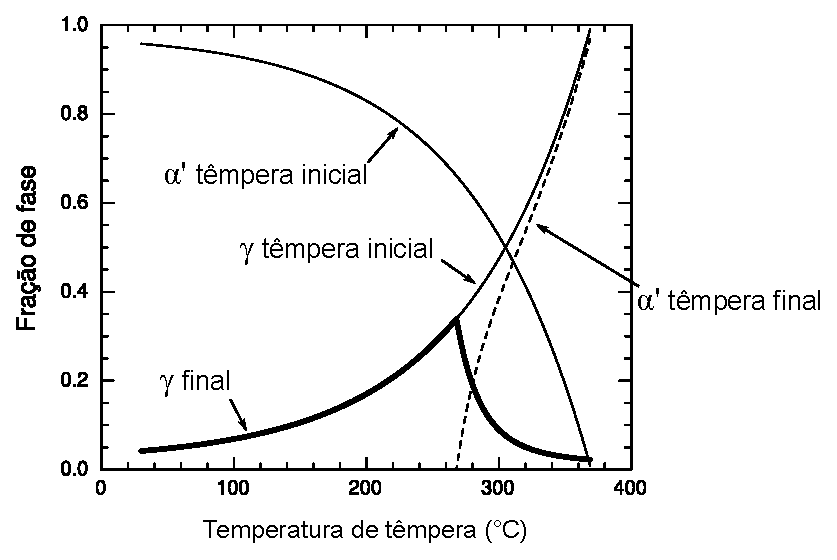
\includegraphics[width=13cm]{img/TPprevisto.pdf}
%   \caption{Predição dos componentes da microestrutura de uma liga Fe-0,4\%C particionada a \SI{300}{\degreeCelsius}. A linha sólida espessa representa a fração de austenita ($\gamma$) ao final do processo T\&P. As demais linhas representam a variação das frações de austenita e martensita ($\alpha'$) após a têmpera inicial e a fração de martensita formada no resfriamento final a partir da austenita não suficientemente estabilizada. Curvas recalculadas a partir da metodologia descrita no texto.}
%   \label{fig:TPprevisto}
% \end{figure}

\subsubsection{Equilíbrio Restringido de Carbono acompanhado de precipitação de carbonetos $(ERC\theta)$}

\novasigla{ERC$\theta$}{Equilíbrio Restringido de Carbono acompanhado de precipitação de carbonetos}

O modelo ERC proposto por Speer requer um conjunto de condições ideais. A interface martensita/austenita deve ser imóvel, os potenciais químicos de carbono na martensita e austenita são iguais e reação competitivas, como a precipitação de carbonetos e a reação bainítica, devem ser totalmente suprimidas. Como ferramenta para planejamento de ligas o modelo ERC se mostrou útil, mas resultados experimentais recentes questionam a validade do modelo para a maioria das aplicações. A migração da interface martensita/austenita tem sido reportadamente observada, direta e indiretamente, por vários autores. A precipitação de carbonetos de transição tem se demonstrado praticamente inevitável para a maioria das ligas submetidas ao processo T\&P e a reação bainítica nem sempre é evitada, nem mesmo em ligas cuidadosamente planejadas. 

\citaremsentenca{Toji2015} propuseram um modelo aprimorado para o entendimento da termodinâmica do processo T\&P ao considerar a mudança da energia livre devido à precipitação de carbonetos. No modelo então chamado de ``Equilíbrio Restringido de Carbono acompanhado de precipitação de carbonetos'', ou ERC$\theta$ (em inglês, \enfase{``Constrained Carbon Equilibrium accompanied by $\theta$ precipitation''}, CCE$\theta$), os carbonetos ($\theta$) precipitados no interior da martensita estabelecem o equilíbrio metaestável com esta fase. A austenita por sua vez, estabelece o equilíbrio local de carbono em relação à mistura martensita + carbonetos. A condição ERC$\theta$ é representada pela construção na Figura \ref{fig:esquema_ERCtheta} para dois carbonetos diferentes com diferentes energia livres. O equilíbrio metaestável entre a martensita e os carbonetos restringe o potencial químico do carbono a um valor fixo. Consequentemente, o potencial químico do carbono na austenita e o teor de carbono na austenita ($w_C^\gamma$) também são forçados a valores constantes. Dessa forma, contrastando o modelo ERC, o carbono na austenita não depende da fração inicial de martensita, mas apenas da energia livre do carboneto precipitado na martensita. Carbonetos menos estáveis (menor energia livre) implicam em maiores concentrações de carbono na austenita, como mostra a construção da Figura \ref{fig:esquema_ERCtheta}. 

\begin{figure}
  \centering  
  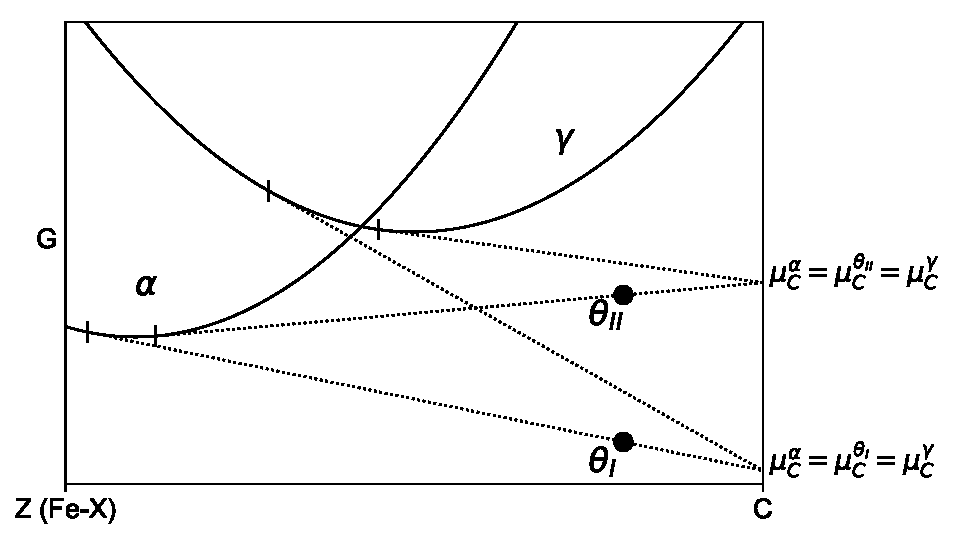
\includegraphics[width=.8\textwidth]{img/common_tangent.pdf}
  \caption{Desenho esquemático ilustrando as configurações de energias livres e potenciais químicos ($\mu_C$) de acordo com o modelo ERC$\theta$.}
  \label{fig:esquema_ERCtheta}
\end{figure}

A aplicação do modelo ERC$\theta$ esbarra no particular desafio da falta de dados termodinâmicos disponíveis sobre as energias livres dos carbonetos de transição. Recentemente, alguns grupos de pesquisa têm tentado determinar as propriedades termodinâmicas de carbonetos de transição por cálculos de primeiros princípios. %CITATION NEEDED
De toda forma, Toji e colaboradores avaliaram o modelo ERC$\theta$ assumindo cementita de ortoequilíbrio (ortocementita) --- isto é, correspondente ao equilíbrio metaestável, formada com partição dos solutos substitucionais ---, cementita de paraequilíbrio (paracementita) e cementita com dissolução parcial de silício.

\subsection{Reações competitivas durante o processo T\&P}

\subsubsection{Precipitação de carbonetos}

% REVISAR CARBONETOS DE TRANSIÇÃO
A precipitação de carbonetos durante a etapa de partição do processo T\&P pode ser interpretada sob o ponto de vista das reações que ocorrem durante o revenimento da martensita. A baixas temperaturas de revenimento é observada a formação de finas dispersões de carbonetos $\epsilon$, de estrutura hexagonal compacta, e dependendo do teor de carbono, também é possível observar carbonetos de estrutura ortorrômbica $\eta$ e $\chi$. No atual entendimento das reações de revenimento é interpretado que estes carbonetos --- por vezes chamados de carbonetos de transição ou intermediários --- subsequentemente se transformam em precipitados de cementita\cite{Speich1972}. %ATUALIZAR REFERENCIAS
Evitar a precipitação de carbonetos é de fundamental importância para se obter quantidades consideráveis de austenita estabilizada por carbono durante o processo T\&P. Por outro lado, carbonetos de transição não são geralmente considerados prejudiciais para as propriedades mecânicas da martensita revenida, embora a formação de cementita seja aspecto de preocupação\cite{Krauss1983}. Dessa forma, é de particular interesse a compreensão dos parâmetros de tratamento térmico e dos efeitos dos elementos de liga na evolução da precipitação de carbonetos durante o processo T\&P. 

É bem estabelecido que o silício possui um papel importante no retardamento da precipitação da cementita a partir da martensita e da austenita e na transição de carbonetos intermediários para cementita. De fato, este é um dos principais conceitos utilizados no desenvolvimento do processo de Têmpera e Partição. Isto acontece devido à solubilidade desprezível do silício na cementita\cite{Owen1951,Barnard1981}, implicando que a cinética da precipitação seja controlada pela expulsão do silício da cementita em crescimento para a fase adjacente. Uma vez que as etapas de revenimento/partição se dão normalmente em baixas temperaturas, a reação é lenta.

É possível argumentar que devido à baixa mobilidade do silício, a precipitação de cementita obedeceria condições de paraequilíbrio e, consequentemente, seria muito mais rápida do que quando a redistribuição de elementos substitucionais acontece.
% No entanto, isto não elimina a evidência experimental de que a precipitação de cementita é retardada na presença de silício.
\citaremsentenca{Ghosh2002} estudaram este possível cenário realizando simulações de cinética de precipitação assumindo condições interfaciais de paraquilíbrio. \citaremsentenca{Kozeschnik2008} também exploraram este possível cenário e teorizaram que o crescimento de paracementita estaria associado a uma redução da força motriz para precipitação, consequentemente implicando em uma cinética mais lenta. Os autores mostraram, também por meio de cálculos cinéticos, que isto de fato ocorre para a precipitação da cementita a partir da austenita, embora o modelo tenha falhado em predizer o mesmo fenômeno na precipitação da cementita a partir da ferrita supersaturada em carbono (martensita). Os autores justificaram o resultado pelo aprisionamento dos átomos de carbono em defeitos cristalinos na martensita, de modo que o fator controlador da reação seria a eliminação dos defeitos para disponibilização do carbono para formação da cementita.

%Discutir\cite{Caballero2008} por aqui, que fez experimentos de APT em carbonetos formados durante o revenimento de bainita. Resultados deles mostram que não há partição de substitucionais durante os primeiros estágios da formação dos carbonetos. A pergunta é: esses carbonetos são cementita ou na verdade são carbonetos de transição?

Embora o silício seja efetivo no retardamento da precipitação da cementita, o mesmo não pode ser dito sobre seu efeito na precipitação dos carbonetos de transição. \citaremsentenca{Owen1954} e \citaremsentenca{Kenneford1957} mostraram que a cinética do primeiro estágio de revenimento, associada à decomposição da martensita em uma mistura de carbonetos $\epsilon$ e martensita de baixo carbono, é pouco afetada pela presença do silício na liga, enquanto a precipitação de cementita em temperaturas mais elevadas é progressiva e consideravelmente atrasada por adições de silício. \citaremsentenca{Reisdorf1963} mostrou por análises de microsonda eletrônica que durante o revenimento de aços contendo 0,4\%C e 1,40\%Si a relação Si:Fe nos carbonetos de revenimento diminui de acordo a transição de carbonetos $\epsilon$ para cementita. Este resultado sinaliza uma maior tolerância dos carbonetos $\epsilon$ ao silício, justificando sua cinética característica. Adicionalmente, a diferença de solubilidades nos carbonetos demanda a partição de silício durante a transição $\epsilon \rightarrow$ cementita.

%Resultados recentes obtidos por tomografia de sonda atômica tridimensional confirmaram este último caso e forneceram informações sobre as condições interfaciais que regem a cinética das reações de precipitação\cite{Zhu2007,Miyamoto2007,Caballero2008}. \citaremsentenca{Miyamoto2007}

%Falar sobre resultados recentes sobre precipitação de carbonetos em materiais temperados e particionados \citaremsentenca{Li2010a} \citaremsentenca{Nayak2008} \citaremsentenca{Edmonds2006}

\subsubsection{Reação bainítica e decomposição da austenita em temperaturas próximas à temperatura Ms}

\label{subsec:decompMs}

A decomposição isotérmica da austenita em temperaturas próximas à temperatura Ms tem sido relatada em uma série de ligas ferrosas. Nestas ligas, uma transformação lenta e isotérmica pode ser observada a baixas temperaturas, ao contrário da cinética rápida, controlada pela nucleação, da martensita atérmica. Diferentes reações são associadas aos produtos formados nesta faixa de temperatura, a citar, a formação de martensita isotérmica a reação bainítica.

A transformação isotérmica da martensita tem sido extensamente estudada em ligas Fe-Ni-Mn em baixas temperaturas\cite{Kaufman1958,Pati1969}. Assim como na formação da martensita atérmica, o crescimento das placas de martensita isotérmica é extremamente rápido, por um mecanismo displacivo, envolvendo uma deformação cisalhante na austenita. Por outro lado, a nucleação deste produto é relativamente lenta, o que permite a determinação das taxas de nucleação envolvidas neste processo\cite{Pati1969}. 

Por sua vez, a observação de martensita isotérmica em ligas contendo carbono é cinética e microestruturalmente associada ao estudo da reação bainítica em temperaturas próximas ao Ms. \citaremsentenca{Howard1947} observaram a formação de bainita em temperaturas inferiores ao Ms em ligas Fe-C e Fe-Ni-C, precedida por um tempo de incubação. Os autores reportaram que em uma liga hipereutetóide houve uma mudança anômala na cinética do início da reação em temperaturas ligeiramente acima do Ms, microestruturalmente associada com a formação de um produto em formato de placa finas. \citaremsentenca{Schaaber1955} determinou por medidas dilatométricas e magnéticas uma reação em dois estágios em temperaturas próximas à temperatura Ms em uma liga Fe-1,16\%C, sugerindo que o primeiro estágio estaria associado à formação de martensita isotérmica, enquanto o estágio subsequente estaria relacionado à reação bainítica.

\citaremsentenca{Radcliffe1959} observaram a ocorrência da aceleração da reação bainítica em temperaturas próximas da temperatura Ms, em ligas hipo e hipereutetóides. Os autores chamaram este fenômeno de \enfase{swing back}. Este fenômeno ocorreria em temperaturas abaixo do Ms em ligas hipoeutetóides e acima do Ms em ligas hipereutetóides. Oka e Okamoto\cite{Okamoto1985,Oka1988} realizaram um estudo sistemático sobre o comportamento da cinética da decomposição da austenita em tratamentos isotérmicos em temperaturas próximas ao Ms em várias ligas Fe-C hipereutetóides, também observando o fenômeno da aceleração da decomposição da austenita nesta faixa de temperaturas. Eles observaram um produto em forma de ``finas linhas pretas'' e, mediante análise cristalográfica, concluíram que a fase consistia de martensita formada isotermicamente. Adicionalmente, Oka e Okamoto também concluíram que a presença deste produto desempenhara papel na formação de bainita inferior e martensita isotérmica lenticular.

Mais recentemente, \citaremsentenca{VanBohemen2008} reportaram evidências de transformação isotérmica da austenita em temperaturas inferiores ao Ms em aços de baixa liga (Mn e Si) e baixo carbono. Kim e colaboradores\cite{Kim2010,Kim2012} relataram a formação de um produto isotérmico em uma liga de baixo carbono durante o processo de Têmpera e Partição. Foram identificadas diferenças morfológicas, cristalográficas e mecânicas entre os produtos isotérmico e atérmico.

A formação de produtos isotérmicos próximos à temperatura Ms é de crucial importância no entendimento da partição de carbono o processo de têmpera e de partição. \citaremsentenca{Clarke2008} analisaram dois possíveis mecanismos de partição de carbono durante o processo T\&P: (i) partição de carbono da martensita supersaturada para a austenita e (ii) formação de bainita isenta de carbonetos. Eles concluíram que as quantidades de austenita observadas experimentalmente são muito superiores àquelas preditas pelo cálculo teórico considerando a formação de ferrita bainítica e que, portanto, o mecanismo de partição de carbono a partir da martensita é mais consistente com os resultados experimentais. Os autores veem a formação de bainita isenta de carbonetos um mecanismo competitivo no sentido de diminuir a fração de austenita durante a etapa de partição.

% ALFONSO
%citar o Raabe aqui.

\simbolo{$\alpha$}{Ferrita}
\simbolo{$\alpha_b$}{Ferrita bainítica}
\simbolo{$\alpha'$}{Martensita}
\simbolo{$\alpha'_{fr}$}{Martensita fresca}
\simbolo{$\gamma$}{Austenita}
\simbolo{MA}{Microconstituinte MA, agregado de austenita retida e martensita fresca}
\simbolo{$\theta$}{Carbonetos}
\simbolo{$Fe_3C$}{Cementita}
\simbolo{$\epsilon$}{Carboneto $\epsilon$}
\simbolo{$\eta$}{Carboneto $\eta$}
\simbolo{$Fe_2O_3$}{Hematita}
\simbolo{$Fe_3O4$}{Magnetita}
\simbolo{$FeO$}{Wüstita}

\simbolo{Ms}{Temperatura de início da transformação martensítica}
\simbolo{Mf}{Temperatura de fim da transformação martensítica}
\simbolo{Md}{Maior temperatura em que a transformação martensítica induzida por deformação é termodinamicamente possível}
\simbolo{$\beta$}{Parâmetro da equação de Koistinen-Marburger que denota a taxa de transformação da austenita para martensita}
\simbolo{Ms'}{Parâmetro da equação de Koistinen-Marburger equivalente à temperatura de início da transformação martensítica}
\simbolo{Bs}{Temperatura acima da qual a transformação bainítica não ocorre}

\simbolo{$T_0$}{Temperatura em que, para uma dada composição, as energias livres da ferrita e austenita são iguais}
\simbolo{$WBs$}{Teor de carbono crítico acima do qual nem ferrita acicular nem ferrita bainítica crescem}
\simbolo{$A_3^{para}$}{Limite de solubilidade de carbono na austenita sob condições de paraequilíbrio}

\simbolo{R}{Constante universal dos gases}
\simbolo{T}{Temperatura}


\chapter{Material e M\'{e}todos}

\section{Material}

O ferro fundido nodular utilizado neste trabalho foi fundido pela empresa Tupy S/A. O material foi fundido na forma de blocos em Y conforme especificação da norma NBR 6916 (figura \ref{fig:nbr6916}) para extração de corpos de prova para ensaios mecânicos. A liga foi fundida em forno de indução a cadinho com capacidade de nove toneladas e operado em frequência de rede. Os blocos foram vazados em moldes confeccionados em processo de caixa fria (areia de sílica com resina fenólica uretânica).

\begin{figure}
	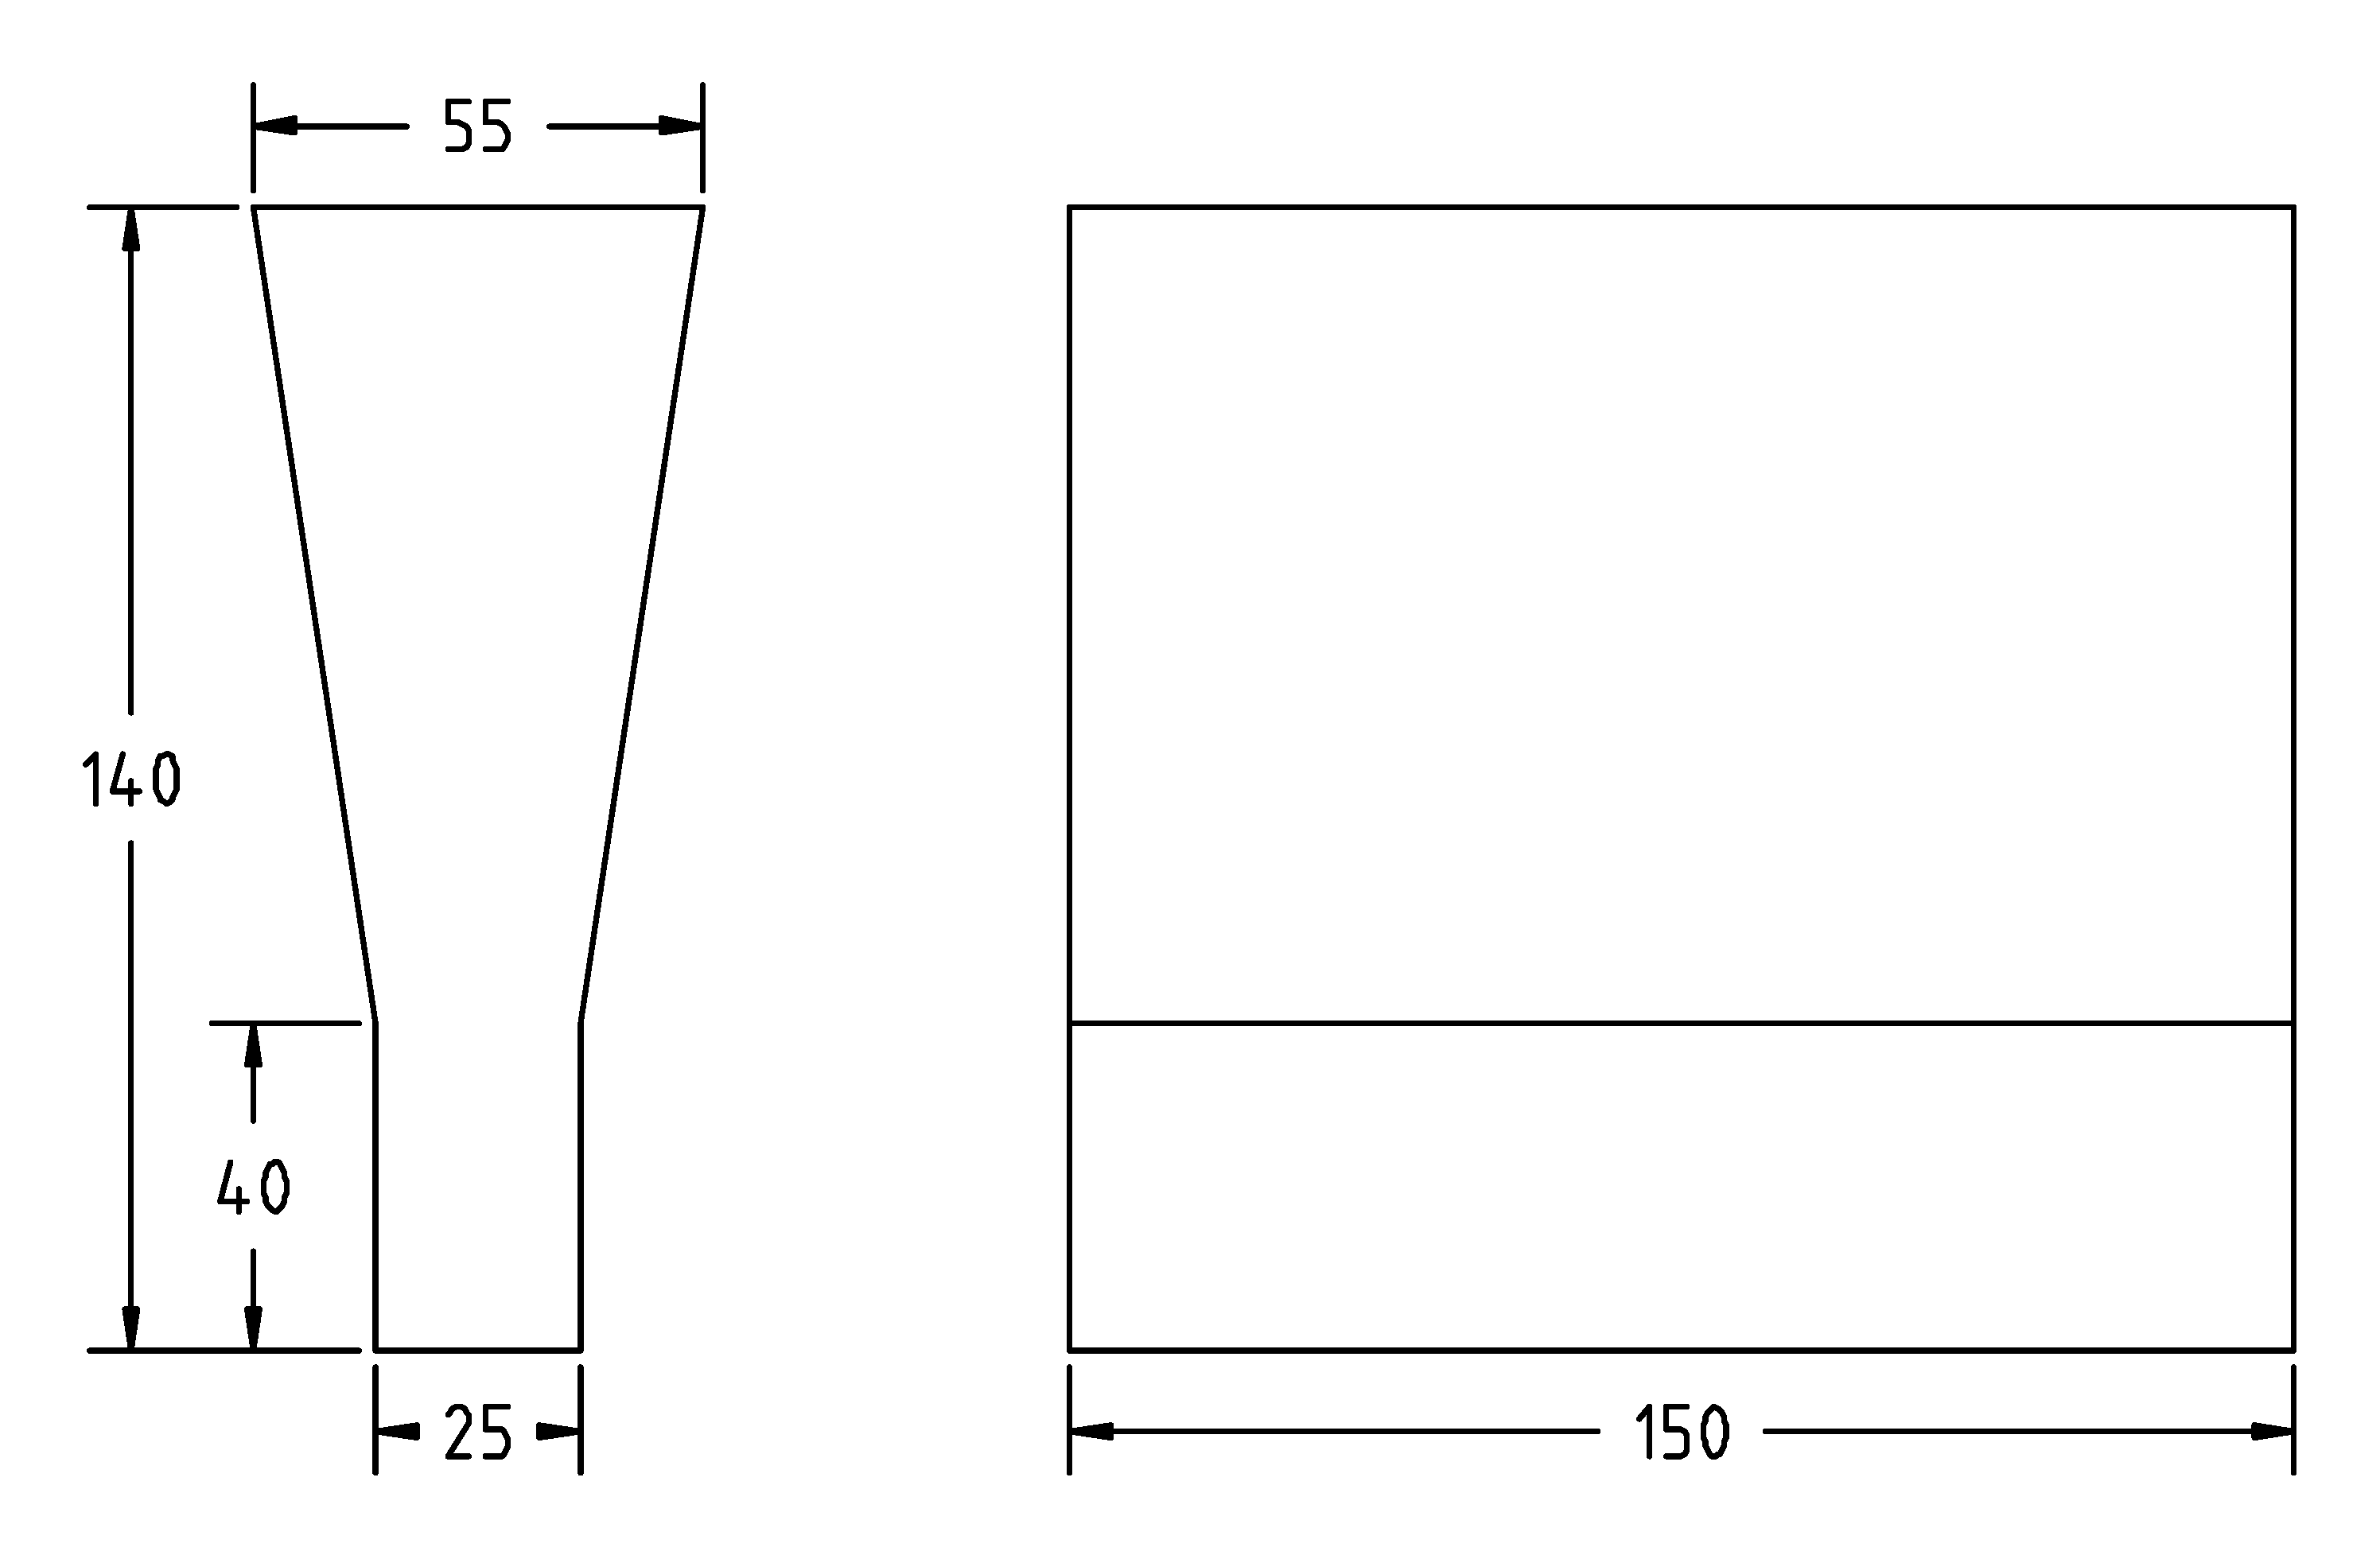
\includegraphics[width=12cm]{img/nbr6916.png}
	\caption{Desenho esquemático do bloco em Y especificado pela norma NBR 6916 para extração de corpos de prova de ensaios mecânicos. Dimensões em milímetros.}
	\label{fig:nbr6916}
\end{figure}

Durante o projeto da liga procurou-se utilizar baixos teores de manganês e o maior grau de inoculação possível. Estas medidas foram tomadas de forma a minimizar a microsegregação inerente ao processo de fundição. Dessa forma, o metal líquido foi submetido a processo de inoculação durante o vazamento e \enfase{em molde}, o que permitiu a obtenção de uma liga com elevada contagem de nódulos de grafita, superior a 400 nódulos/mm\textsuperscript{2}. A composição química da liga é dada na tabela \ref{tab:CQ}. %será que eu falo a contagem de nódulos obtida aqui ou na parte de resultados?

\begin{table}
	\caption{Composição química da liga fundida (\% em massa).}
	\begin{tabular}{c c c c c c c c c}
	\thickhline
	\textbf{Elemento} & C & Si & Mn & Cu & Cr & Mg & P & S \\
	\hline
	\textbf{Composição (\% em massa)} & 3,47 & 2,47 & 0,20 & 0,38 & 0,03 & 0,03 & 0,04 & 0,01 \\
	\thickhline
	\end{tabular}
	\label{tab:CQ}
\end{table}

\section{Metodologia}

\subsection{Determina\c{c}\~{a}o dos par\^{a}metros de tratamento t\'{e}rmicos}

Este estudo se limitou a avaliar o efeito das variáveis ``temperatura de têmpera'' e ``temperatura de partição'' na microestrutura do produto final, na cinética de redistribuição de carbono durante a etapa de partição e na retenção de austenita retida após o processo T\&P. Nesta avaliação, as demais variáveis de tratamento térmico, tal qual a ``temperatura de austenitização'', foram mantidas fixas.

\subsubsection*{Temperatura de austenitização (TA)} \simbolo{TA}{Temperatura de austenitização}

A determinação da temperatura de austenitização do material foi feita utilizando abordagem teórica e experimental. Simulações feitas no software de termodinâmica computacional Thermo-Calc\textregistered{} foram utilizadas para estimar a faixa de temperaturas em que é estabelecido o equilíbrio entre austenita e grafita, na qual é dada a austenitização plena do material. A escolha de uma temperatura muito elevada poderia levar à liquação de regiões do material durante o tratamento térmico. Por outro lado, a escolha de uma temperatura muito baixa poderia levar à austenitização incompleta do material, introduzindo uma variável experimental indesejada.

Adicionalmente, uma amostra de ferro fundido foi submetida a um ensaio de dilatometria no dilatômetro Bähr 805A para determinação das temperaturas críticas de transformação do material. A amostra foi aquecida até a temperatura de 880 °C a uma taxa de aquecimento de 10 °C/min, em que foi mantida por 5 min antes do resfriamento final a uma taxa de --50 °C/s. Mais detalhes sobre as configurações do ensaio de dilatometria são apresentados na seção \ref{subsec:dilatometria}. Os resultados deste experimento preliminar foram comparados com os resultados da abordagem feita pelo software Thermo-Calc\textregistered{}.

O tempo de austenitização escolhido foi de 1800 segundos (30 minutos). Embora alguns trabalhos na literatura utilizem tempos mais prolongados para a austenitização plena de ferros fundidos \cite{Trudel1997}, foi considerado que, devido ao alto grau de inoculação da liga estudada (cerca de quatro vezes maior do que o utilizado em ligas comerciais), o tempo empregado neste trabalho pode ser considerado suficiente para dissolução das fases presentes na matriz do material como recebido.

%Talvez falar porque escolhi a menor temperatura de austenitização plena.

\subsubsection*{Temperaturas de t\^{e}mpera (TT)} \simbolo{TT}{Temperatura de têmpera}

Como objeto de estudo, foram escolhidas três diferentes temperaturas de têmpera para realização dos tratamentos térmicos: 140, 170 e 200 °C. Procurou-se garantir que as três temperaturas utilizadas fossem menores que a temperatura Ms, de modo que quantidades substanciais de martensita atérmica fossem produzidas durante a etapa de têmpera. Por sua vez, a determinação da temperatura Ms foi feita preliminarmente por meio de um ensaio de dilatometria que reproduziu o ciclo de austenitização e têmpera.

\subsubsection*{Temperaturas de parti\c{c}\~{a}o (TP)} \simbolo{TP}{Temperatura de partição}

Cinco diferentes temperaturas de partição foram utilizadas neste estudo: 200, 250, 300, 375 e 450 °C. As condições de 300, 375 e 450 °C foram utilizadas por serem comumente reportadas como parâmetros para os tratamentos isotérmicos na produção do ferro fundido nodular austemperado. %citar referências
Por sua vez, as temperaturas de 200 e 250 °C foram escolhidas por serem próximas à temperatura Ms determinada experimentalmente. Consequentemente, para estas condições poderiam ser esperadas reações competitivas semelhantes às reportadas na seção \ref{subsec:decompMs}.

\subsection{Experimentos de dilatometria}

\label{subsec:dilatometria}

Ensaios de dilatometria foram realizados para a determinação da temperatura Ms da liga estudada, como mencionado anteriormente, e para simular os ciclos térmicos correspondentes aos tratamentos de T\&P. Os resultados de dilatometria forneceram informações para identificação das temperaturas de início e fim das transformações de fases durante as etapas de aquecimento e resfriamento e para determinação da cinética das transformações que ocorrem nas etapas isotérmicas do processo T\&P. Os experimentos foram realizados no dilatômetro de têmpera Bähr DIL805A, localizado nas dependências do Departamento de Engenharia Metalúrgica e de Materiais da EPUSP. No dilatômetro o aquecimento das amostras é feito por indução eletromagnética utilizando uma bobina de cobre refrigerada a água e o controle da temperatura é feito por meio de termopares tipo S (Pt/Pt-Rh) soldados às amostras.

Amostras cilíndricas de 10 mm de comprimento e 4 mm de diâmetro (figura \ref{fig:CPdil}a) foram utilizadas para simular o processo de têmpera e partição nas condições estudadas. As amostras foram usinadas a partir da região central da parte útil do bloco em Y, primeiramente por extração por eletroerosão de varetas de 4 mm de diâmetro e em seguida por corte e faceamento para estabelecimento do comprimento útil de 10 mm.

\begin{figure}
	\subfloat[]{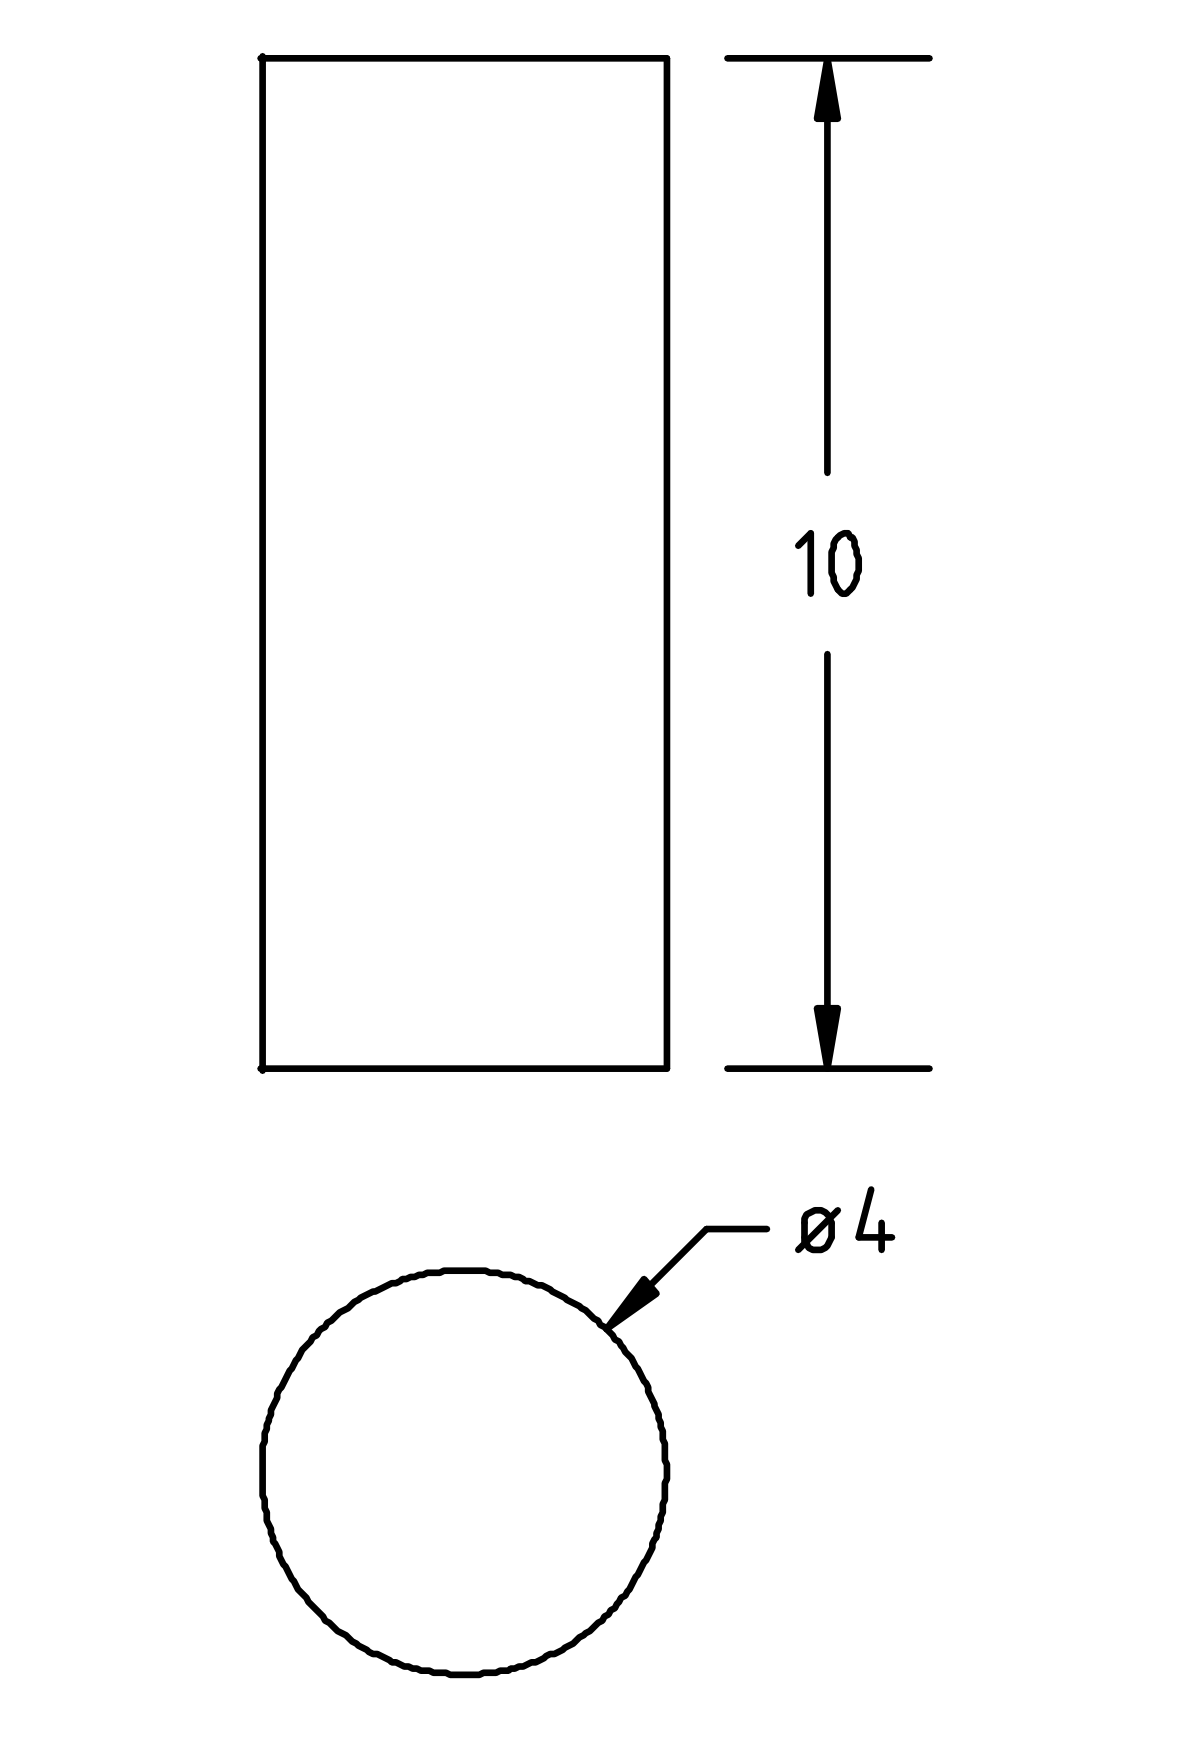
\includegraphics[height=7cm]{img/CPdil.png}}
	\hspace{5em}
	\subfloat[]{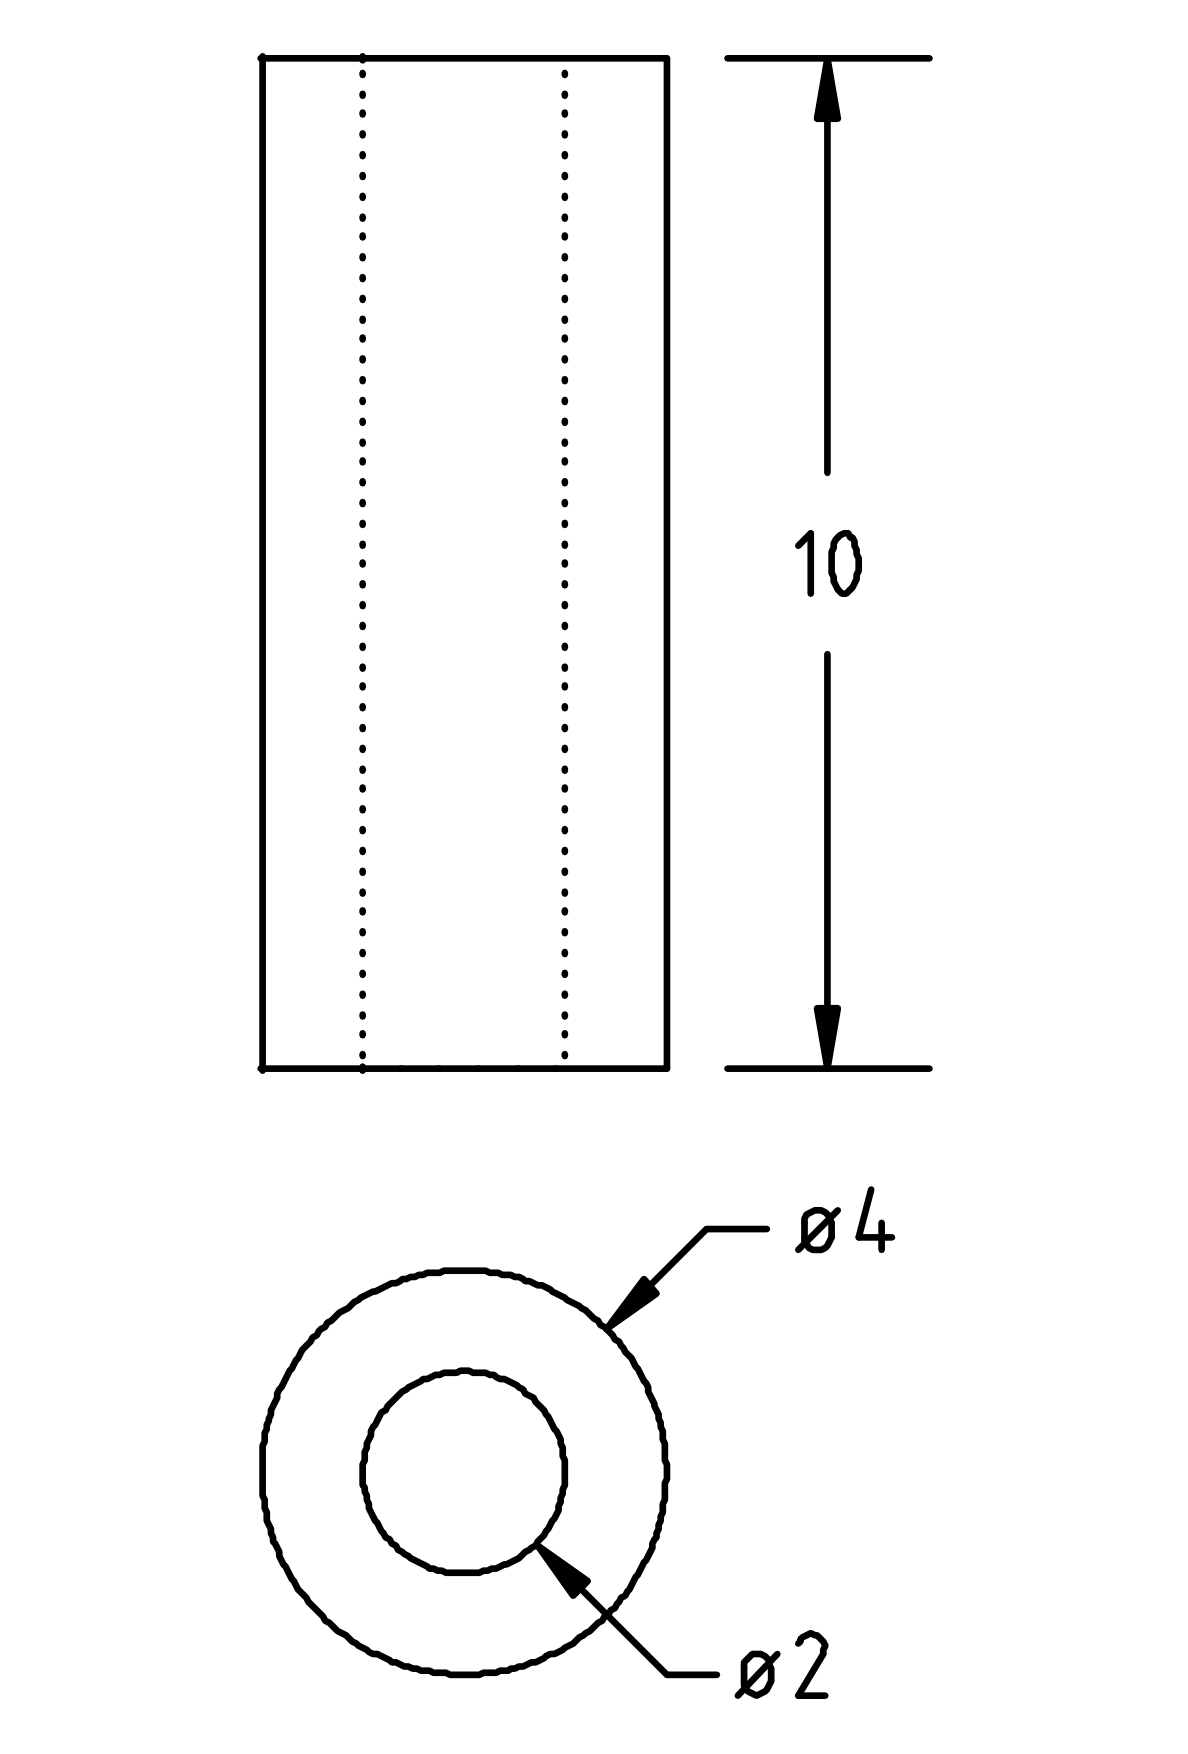
\includegraphics[height=7cm]{img/CPdil_subzero.png}}
	\caption{Desenhos esquemáticos dos corpos de prova de dilatometria. (a) Amostra cilíndrica para simulação de tratamentos T\&P. (b) Amostra no formato de cilindro oco para experimentos subzero. Dimensões em milímetros.}
	\label{fig:CPdil}
\end{figure}

O ciclo térmico empregado nos ensaios de dilatometria consistiu da austenitização das amostras por 1800 segundos, seguido de rápido resfriamento até as temperaturas de têmpera (TT) e reaquecimento até as temperaturas de partição (TP), nas quais as amostras foram mantidas por 900 segundos. As etapas de aquecimento foram realizadas sob taxa de 10 °C/s, enquanto a têmpera foi feita a --50 °C/s utilizando resfriamento forçado por gás hélio. A figura \ref{fig:expDil} representa esquematicamente o ciclo térmico de Têmpera e Partição utilizado ensaios nestes.

\begin{figure}
	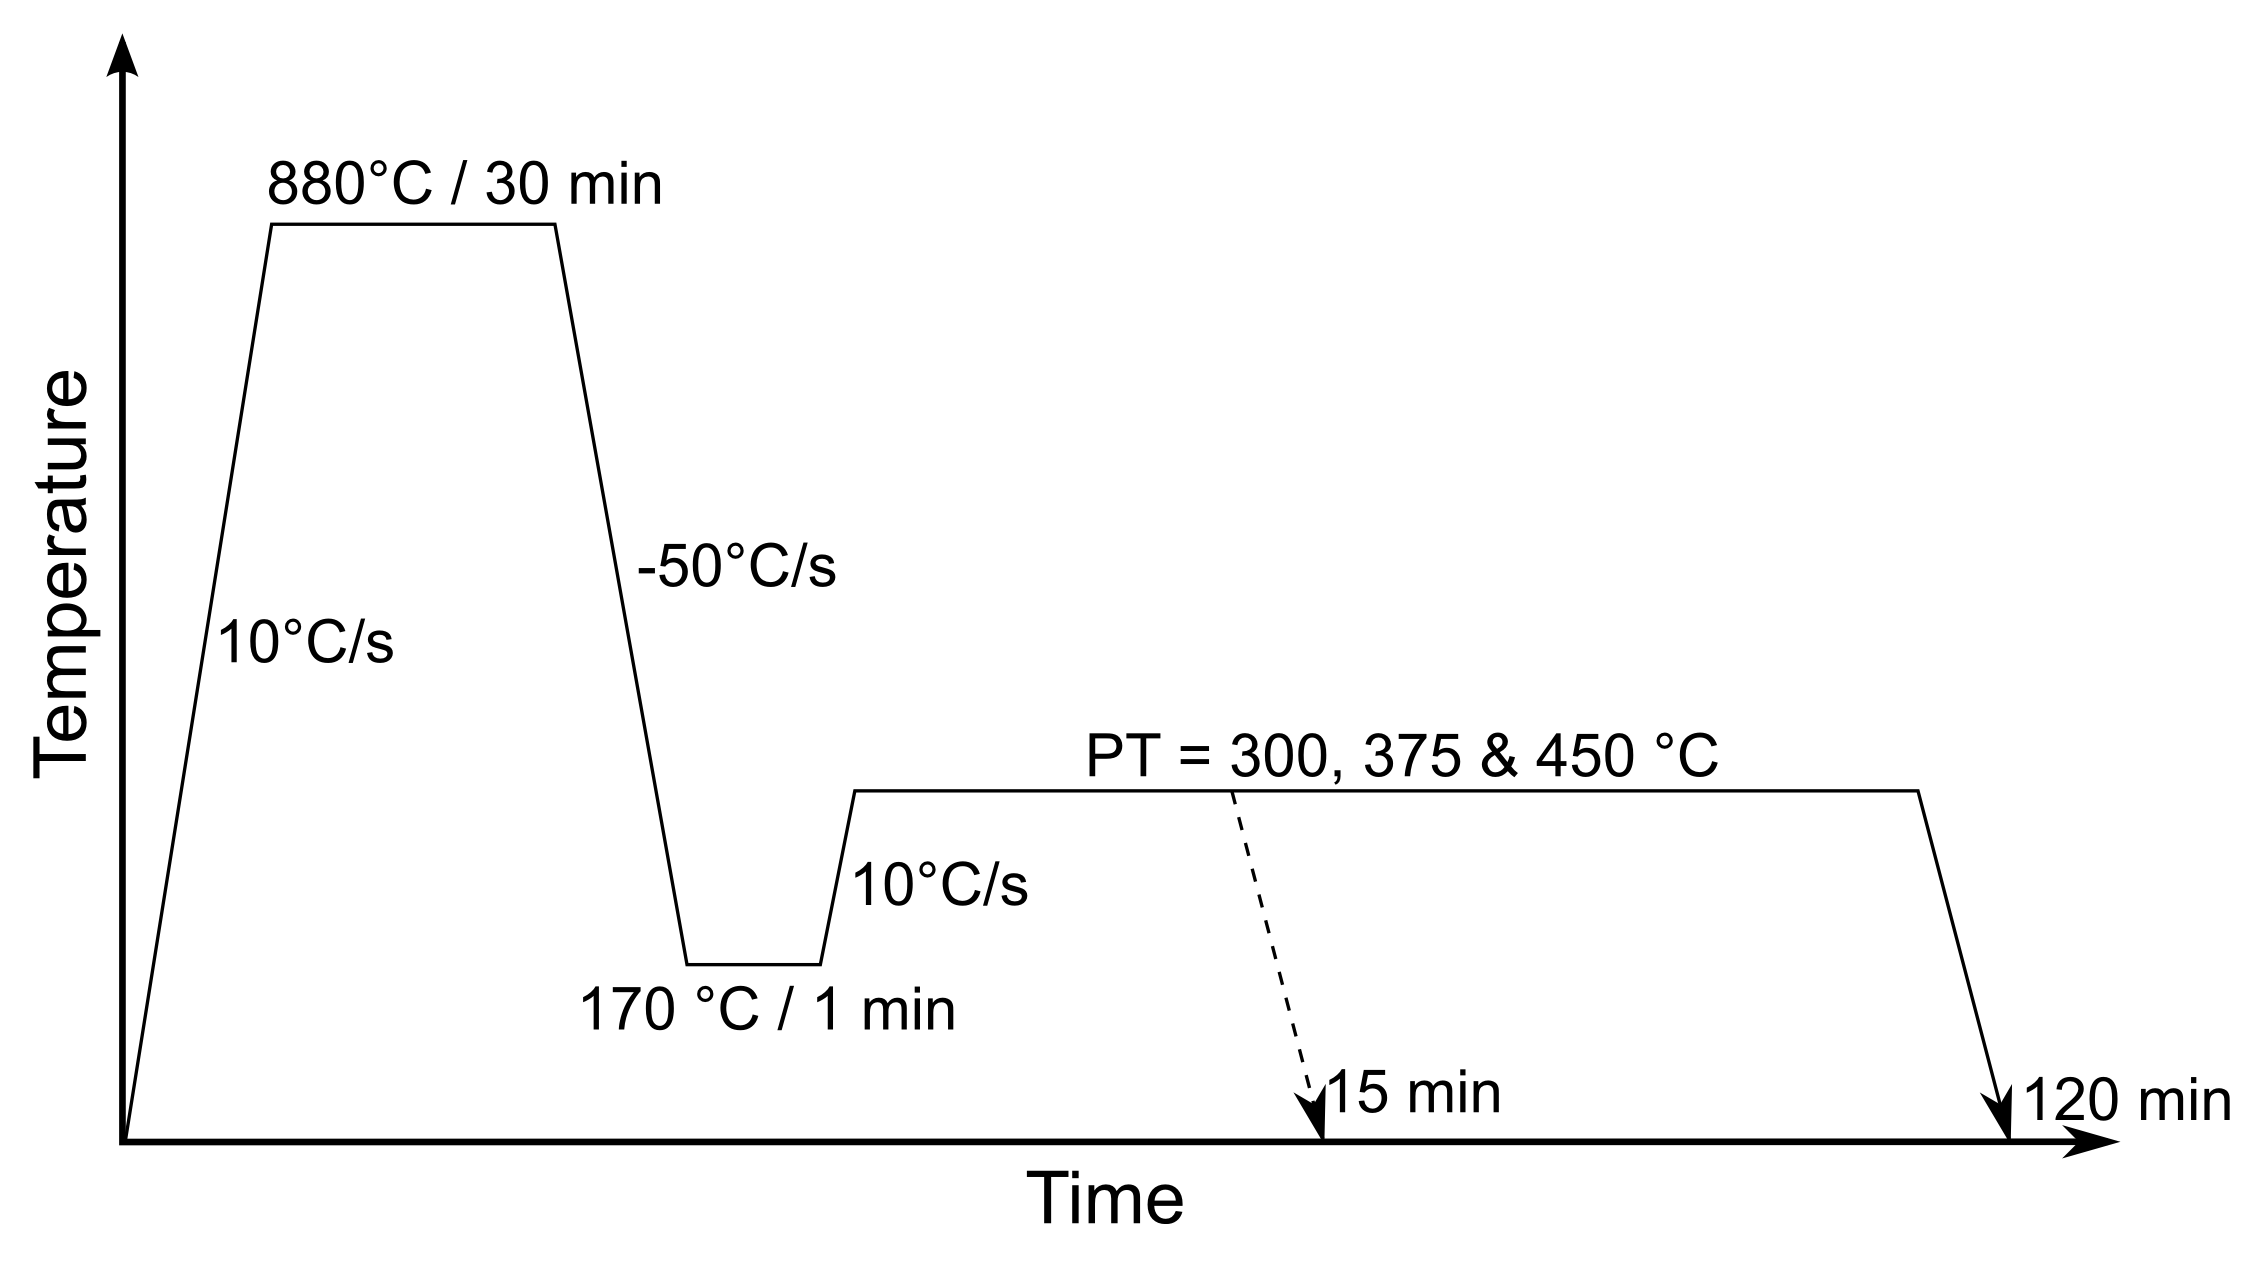
\includegraphics[height=8cm]{img/expproc_dil.png}
	\caption{Ilustração esquemática do ciclo térmico de Têmpera e Partição aplicado nas amostras de dilatometria.}
	\label{fig:expDil}
\end{figure}

O experimento para determinação da temperatura Ms consistiu do aquecimento da amostra até a temperatura de austenitização selecionada, seguindo rampa de aquecimento de 10 °C/s, sendo mantida nesta temperatura por 1800 segundos. Em seguida, a amostra foi resfriada até a temperatura de -100 °C sob taxa de resfriamento de --50 °C/s utilizando gás He refrigerado por $N_2$ líquido. O resfriamento até esta temperatura permitiu que a curva da transformação martensítica fosse completamente determinada. Para que o resfriamento até temperaturas abaixo de zero pudesse ser realizado no equipamento, a geometria da amostra utilizada foi de cilindro oco, como representado na figura \ref{fig:CPdil}b.

\subsection{Difra\c{c}\~{a}o de raios X \enfase{in situ}}

Tratamentos térmicos com acompanhamento em tempo real (\enfase{in situ}) da evolução de fases por difração de raios X gerados por fonte de luz síncrotron foram realizados na estação experimental \siglaestrangeira{XTMS}{X-ray Scattering and Thermo-Mechanical Simulation}, operada pelo \sigla{LNNano}{Laboratório Nacional de Nanotecnologia} com suporte do \sigla{LNLS}{Laboratório Nacional de Luz Síncrotron} na cidade de Campinas. A instalação da linha XTMS consiste de um avançado simulador termomecânico especialmente construído para ser usado em experimentos de difração de raios X. O simulador, chamado de Gleeble\textregistered{} 3S50, foi desenvolvido em cooperação da empresa estadunidense \siglaestrangeira{DSI}{Dynamic Systems Inc.} e de corpo técnico-científico do LNLS e do LNNano para o propósito de efetuar testes termomecânicos com controle de temperatura e solicitação mecânica em amostras macroscópicas, enquanto aquisições simultâneas de difração de raios X são efetuadas. %A figura xx mostra a configuração da instalação no blablabla

No interior da câmara do simulador Gleeble os corpos de prova são presos por garras de cobre, por meio das quais é conduzida corrente elétrica para aquecimento das amostras por efeito Joule. O controle da potência é feito por algoritmo proporcional integral derivativo (PID), sendo que a resposta de temperatura é obtida por meio de termopares (tipo K) soldados às amostras.

A instalação conta com um goniômetro de alta resolução montado ao redor do simulador. O goniômetro é montado sobre uma mesa de alinhamento que permite o posicionamento do plano de difração sobre a superfície da amostra. Os detetores para contagem de fótons ficam localizados no goniômetro e podem ser posicionados em ângulos entre 0 e 150° e a uma distância mínima da superfície da amostra de 361 mm. Neste trabalho, foram utilizados dois detetores Mythen 1K, cada um possuindo 1280 canais de aquisição (pixels) de 50 $\mu$m de largura. Na distância mínima de trabalho, cada detetor cobre uma faixa de ângulos de aproximadamente 10°, totalizando um ângulo de cobertura de cerca de 20°.

Para os experimentos, corpos de prova do ferro fundido foram usinados na geometria esquematizada na figura \ref{fig:CPXTMS}. Durante o posicionamento das amostras no interior da câmara do simulador procurou-se estabelecer o ângulo $\omega$ de 15° entre a superfície da amostra e o feixe incidente de raios X. Em sequência, as amostras foram submetidas a ciclos de Têmpera e Partição segundo as condições de tratamento térmico pré-determinadas.

\simbolo{$\omega$}{Ângulo estabelecido entre o feixe de raios X incidente e a superfície da amostra}

Assim como nos ensaios de dilatometria realizados no dilatômetro Bähr, as amostras foram austenitizados durante 30 min, resfriadas até as temperaturas de têmpera e em seguida reaquecidas até as temperaturas de partição, em que foram mantidas durante 1800 segundos. Nas etapas de resfriamento não foi utilizado resfriamento forçado por meio convectivo, de modo que a extração de calor foi feita unicamente por meio das garras de cobre em contato com os corpos de prova. Consequentemente, taxas de resfriamento inferiores às obtidas no dilatômetro Bähr foram conseguidas no simulador Gleeble.

\begin{figure}
	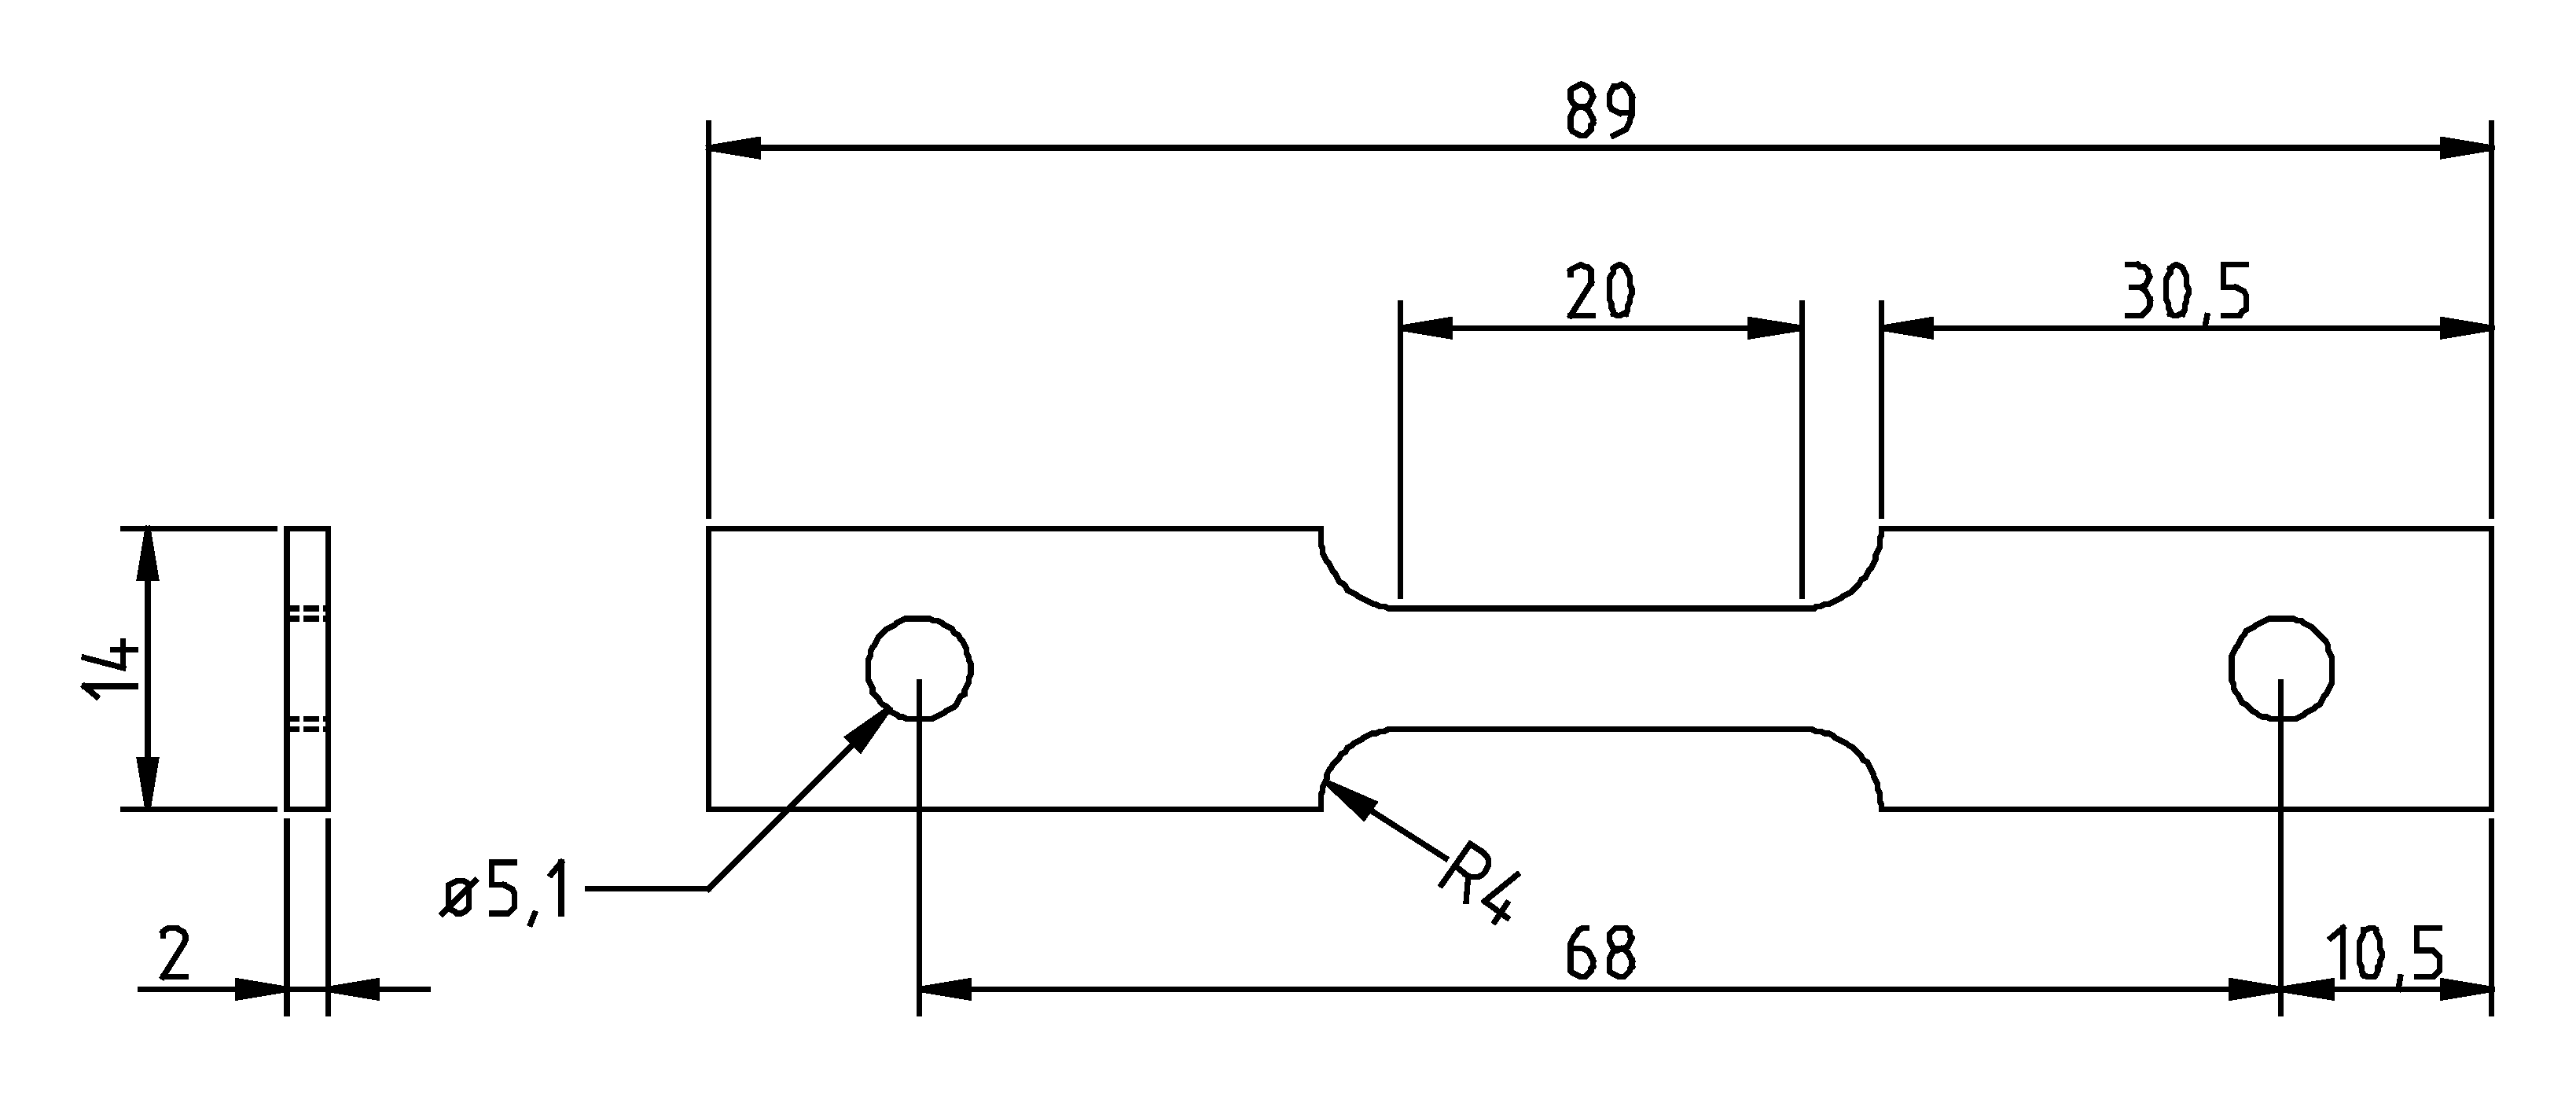
\includegraphics[width=14cm]{img/CPXTMS.png}
	\caption{Desenho esquemático do corpo de prova utilizado na estação experimental XTMS. Dimensões em  milímetros.}
	\label{fig:CPXTMS}
\end{figure}

Paralelamente à realização dos tratamentos térmicos foram feitas aquisições de difração de raios X. A energia do feixe foi estabelecida em 12 keV, equivalente ao comprimento de onda $\lambda = 1,033\text{\AA}$, utilizando monocromador de Si(111). As fendas de limitação de fluxo de fótons foram ajustadas para permitirem que apenas uma região de 2 x 0,5 mm\textsuperscript{2} do feixe incidisse sobre a superfície da amostra. Durante as aquisições em tempo real, o goniômetro foi fixado no ângulo 2$\theta$ de 31° e os detetores Mythen foram aproximados até a distância mínima de trabalho de 361 mm. Nesta configuração, os detetores cobriram a faixa de ângulos de difração de 26 a 47°, na qual foi possível monitorar a evolução dos picos de difração (110) e (200) da ferrita e (111) e (200) da austenita.

\simbolo{2$\theta$}{Ângulo de difração} %definir tth melhor aqui.

Dependendo da etapa do tratamento térmico, foram utilizados diferentes tempos e frequências de aquisição de dados. Durante a etapa isotérmica de partição, aquisições foram feitas a cada 3,5 segundos, utilizando o tempo de exposição de 3 segundos. Ao final da etapa de partição e do tratamento térmico foram feitas varreduras do ângulo de difração entre 26 e 86° a 10 segundos de exposição por passo, de modo a obter um número de picos de difração substantivo para quantificação das fases. A figura \ref{fig:esqXTMS} ilustra a programação do experimento na instalação XTMS.

\begin{figure}
	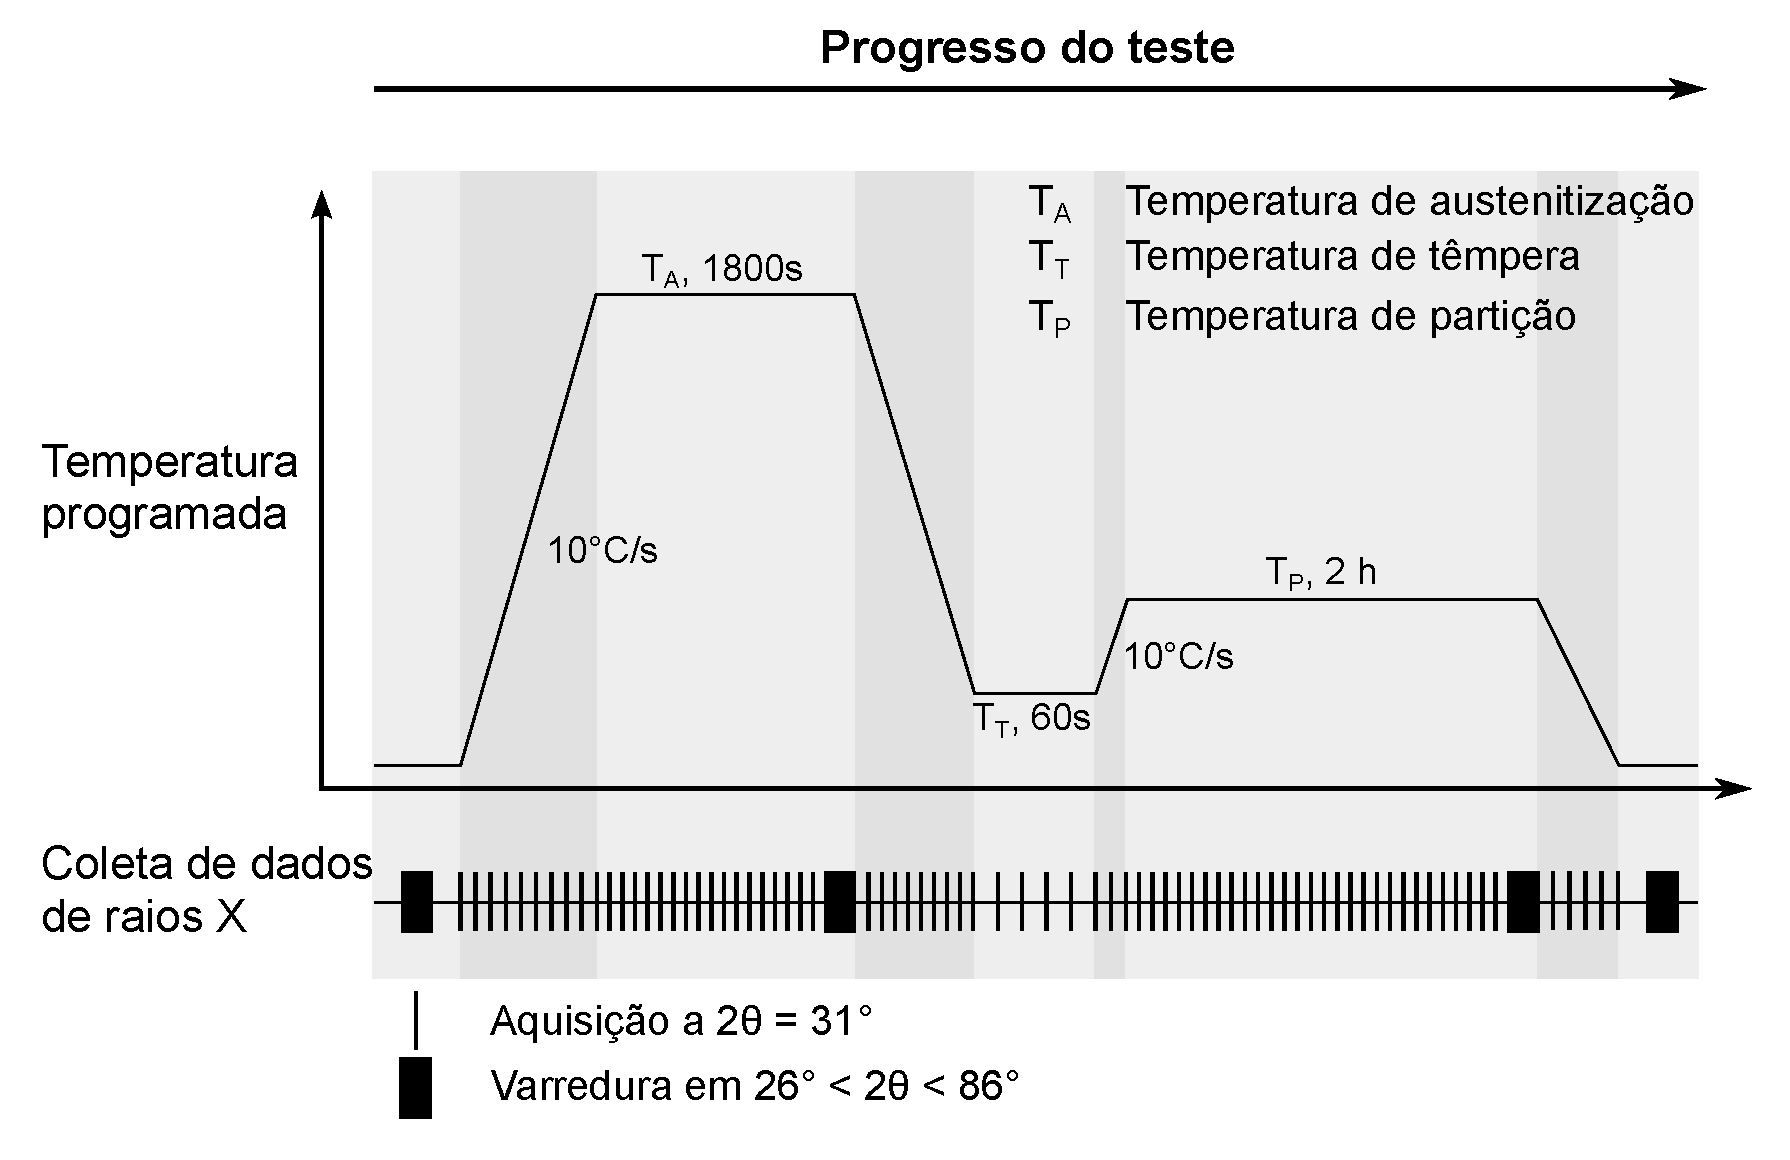
\includegraphics[height=10cm]{img/expproc_XTMS.png}
	\caption{Ilustração esquemática do teste programado na instalação XTMS.}
	\label{fig:esqXTMS}
\end{figure}

Antes de cada experimento a câmara do simulador Gleeble foi evacuada por um sistema de vácuo composto de bomba mecânica e difusora. Os níveis de vácuo atingidos foram consistentemente inferiores a $1 \times 10^{-2}$ torr. Um bom nível de vácuo é imprescindível para que a oxidação e a descarbonetação do material em sua superfície sejam evitadas durante o aquecimento e a aquisição dos difratrogramas.

\subsubsection{An\'{a}lise dos resultados de DRX}

Uma vez que a amostra fica posicionada em um ângulo fixo em relação ao feixe de raios X, a geometria de difração $\omega$--$2\theta$ utilizada difere fundamentalmente das geometrias convencionais dos métodos de Bragg-Brentano ($\theta$--$2\theta$) e Debye-Scherrer (feixe transmitido). A interpretação dos padrões de difração, no entanto, seguiu procedimentos semelhantes de indexação e determinação dos parâmetros de rede das fases.

A análise dos difratogramas obtidos durante os tratamentos isotérmicos foi feita utilizando uma rotina programada no software WaveMetrics IGOR Pro\textregistered{} por \citaremsentenca{Babu2005}. Os picos de difração obtidos foram ajustados segundo a equação de distribuição Gaussiana dada por:

\begin{equation}
	I = I_0 \exp{\left[-\left(\frac{2\theta - 2\theta_0}{w}\right)^2\right]} + bck
	\label{eq:Gaussiana}
\end{equation}
%
em que $I$ corresponde à intensidade de difração observada em função do ângulo $2\theta$, $I_0$ é a intensidade máxima medida no ângulo de difração $2\theta_0$, $w$ é a largura do pico Gaussiano e $bck$ contabiliza o ruído de fundo (\enfase{background}), que tem seu valor assumido como constante. As áreas integradas ($A_{hkl}$) sob os picos foram calculadas pela integração da curva Gaussiana usando a equação \ref{eq:intGauss}, sendo convertidas para frações volumétricas de fases pela equação \ref{eq:fracDRX}, conforme metologia descrita por \citaremsentenca{Cullity2001}.

\begin{align}
	A &= \int\limits_{-\infty}^{\infty} I_0 \exp{\left[-\left(\frac{2\theta - 2\theta_0}{w}\right)^2\right]} d \theta \nonumber \\
	&= I_0 |w| \sqrt{\pi}
	\label{eq:intGauss}
\end{align}

\begin{equation}
	f^\gamma = 1 - f^\alpha = \frac{\sum A_{hkl}^\gamma/R_{hkl}^\gamma}{\sum A_{hkl}^\alpha/R_{hkl}^\alpha + \sum A_{hkl}^\gamma/R_{hkl}^\gamma}
	\label{eq:fracDRX}
\end{equation}

A equação \ref{eq:fracDRX} faz uso dos coeficientes $R_{hkl}$ que contabilizam o efeito dos fatores que compõem o cálculo da intensidade teórica dos picos de difração. Na tabela \ref{tab:fatoresR} são apresentados os valores de $R_{hkl}$ utilizados para quantificação das fases neste trabalho.

\begin{table} %REVISAR ANTES DE IMPRIMIR!
	\caption{Coeficientes $R_{hkl}$ calculados para as fases ferrita ($\alpha$) e austenita ($\gamma$) do ferro puro\cite{Cullity2001}.}
	\begin{tabular}{c c c ' c c c}
	\thickhline
	Fase & hkl & $R_{hkl}$ & Fase & hkl & $R_{hkl}$\\
	\hline
	& 110 & 1840 & & 111 & 1351\\
	& 200 & 288,6 & & 200 & 644,3\\
	$\alpha$ & 211 & 530,0 & $\gamma$ & 220 & 376,7\\
	& 220 & 142,5 & & 311 & 390\\
	& 310 & 172,8 & & 222 & 107,9\\
	\thickhline
	\end{tabular}
	\label{tab:fatoresR}
\end{table}

A variação do parâmetro de rede da austenita ao longo do tratamento isotérmico também foi avaliada pelos resultados de DRX. A partir do cálculo do espaçamento interplanar $d_{hkl}$ pela lei de Bragg (equação \ref{eq:Bragg}), o parâmetro de rede da austenita $a^\gamma$ foi determinado pela equação \ref{eq:parametroRede}, que, para sistemas cristalinos cúbicos, estabelece a relação entre o parâmetro de rede da fase e a distância interplanar entre planos de índices de Miller $hkl$.

\begin{equation}
	n\lambda = 2d_{hkl}\,sen(\theta_0)
	\label{eq:Bragg}
\end{equation}

\begin{equation}
	d_{hkl}^\gamma = \frac{a^\gamma}{\sqrt{h^2 + k^2 + l^2}}
	\label{eq:parametroRede}
\end{equation}

A variação do parâmetro de rede foi interpretada pelo enriquecimento em carbono da austenita durante a etapa de partição do tratamento T\&P. Dessa forma, a variação do teor de carbono foi estimada por meio da equação empírica obtida por \citaremsentenca{Dyson1970}, que leva em conta a variação do parâmetro de rede da austenita em função de sua composição química:

\begin{equation}
	a^\gamma = 3,5780 + 3,30\cdot10^{-2} \%w_C^\gamma + 9,5\cdot10^{-4} \%w_{Mn}^\gamma + 1,5\cdot10^{-3} \%w_{Cu}^\gamma
	\label{eq:DysonHolmes}
\end{equation}
%
em que $\%w_i^\gamma$ é a porcentagem em massa do elemento $i$ (= C, Mn, Cu) dissolvido na austenita. A equação original também descreve a contribuição de outros elementos no parâmetro de rede da austenita. No entanto, suas representações na equação acima foram poupadas, devido a seus baixos teores na liga estudada. Dyson e Holmes argumentam que o silício, que aparece em quantidade substancial no ferro fundido, apresenta efeito desprezível na distorção do reticulado da austenita e, portanto, sua contribuição não é incorporada à equação.

Uma vez que as aquisições foram feitas a temperaturas elevadas, para que os valores de $a^\gamma$ obtidos pelos difratogramas pudessem ser interpretados na temperatura ambiente pelo método descrito acima, previamente à aplicação da equação \ref{eq:DysonHolmes}, o efeito da expansão térmica no parâmetro de rede da austenita foi corrigido utilizando a equação desenvolvida por \citaremsentenca{VanBohemen2013b}:

\begin{equation}
	\frac{\Delta L^\gamma}{L_0^\gamma} = B_\gamma T + B_\gamma \Theta_D^\gamma \left[ \exp{\left( -\frac{T}{\Theta_D^\gamma} \right)}\right]
	\label{eq:expTermica}
\end{equation}

A equação \ref{eq:expTermica} descreve a variação de comprimento $\Delta L^\gamma$ de uma amostra completamente austenítica na temperatura absoluta $T$ em relação a seu comprimento $L_0^\gamma$ extrapolado para o estado de referência a 0 K. $B^\gamma$ e $\Theta_D^\gamma$ são constantes de ajuste determinadas pela regressão linear de dados disponíveis na literatura e valem $B^\gamma = 24,8 \times 10^{-6} K^{-1}$ e $\Theta_D^\gamma = 280 K$.

\subsection{Caracteriza\c{c}\~{a}o microestrutural}

Para análise da microestrutura das amostras, estas foram submetidas a preparação metalográfica, que consistiu do embutimento das amostras em baquelite, lixamento em lixa d'água até granulometria 1200 e subsequente polimento em pastas de diamante de 6, 3 e 1 $\mu$m. Por fim, as amostras foram submetidas a ataques metalográficos com reagentes químicos adequados para cada propósito. Para observação no microscópio óptico, as amostras foram pré-atacadas com o reagente Nital 2\% ($etanol + 2\%vol\,HNO_3$), sendo logo em seguida lavadas sob água corrente com detergente neutro e algodão, e subsequentemente imersas em solução do reagente Beraha ($3g\,K_2S_2O_5 + 10g\,Na_2S_2O_3 + 100mL\,H_2O$) por 60 segundos. O reagente Beraha, assim como outros reagentes que produzem ataques seletivos em ligas ferrosas, colore a ferrita, deixando-a marrom quando observada no microscópio óptico. De forma semelhante acontece com a martensita, que se apresenta amarelada sob ação deste reagente. Por sua vez, a austenita fica isenta do ataque e, consequentemente, aparece branca nas micrografias\cite{MetalsVol9}. Para observação no \sigla{MEV}{Microscópio Eletrônico de Varredura}, as amostras foram apenas atacadas utilizando o reagente Nital 2\%.

Para obtenção de imagens de microscopia óptica foi utilizado o microscópio óptico Olympus BX60M com câmera CCD acoplada, localizado nas dependências do \sigla{LCMHC}{Laboratório de Caracterização Microestrutural Hubertus Colpaert} do \sigla{PMT-USP}{Departamento de Engenharia Metalúrgica e de Materiais da EPUSP}. As imagens de microscopia eletrônica de varredura foram obtidas tanto no microscópio de feixe de emissão de campo (MEV-FEG) FEI Inspect F50 com sistemas de \sigla{EDS}{Análise de Energia Dispersiva} e \sigla{EBSD}{Difração de Elétrons Retroespalhados} acoplados a ele. Estes equipamentos estão situados no \sigla{LabMicro}{Laboratório de Microscropia Eletrônica e de Força Atômica}, também vinculado ao PMT-USP.

\novasigla{MEV-FEG}{Microscópio Eletrônico de Varredura de Feixe de Emissão de Campo}

\section{Resultados e discussão}

\AtBeginSubsection[]{
  \begin{frame}<beamer>{Sumário}
    \tableofcontents[currentsection,currentsubsection]
  \end{frame}
}

\AtBeginSubsubsection[]{
  \begin{frame}<beamer>{Sumário}
    \tableofcontents[currentsection,currentsubsection,currentsubsubsection]
  \end{frame}
}

%%%%%%%%%%%%%%%%%%%%%%%%%%%%%%%%%%%%%%%%%%

\subsection{Características microestruturais pré etapa de partição}

\begin{frame}{Transformação martensítica}
  \only<1>{
    \begin{figure}
      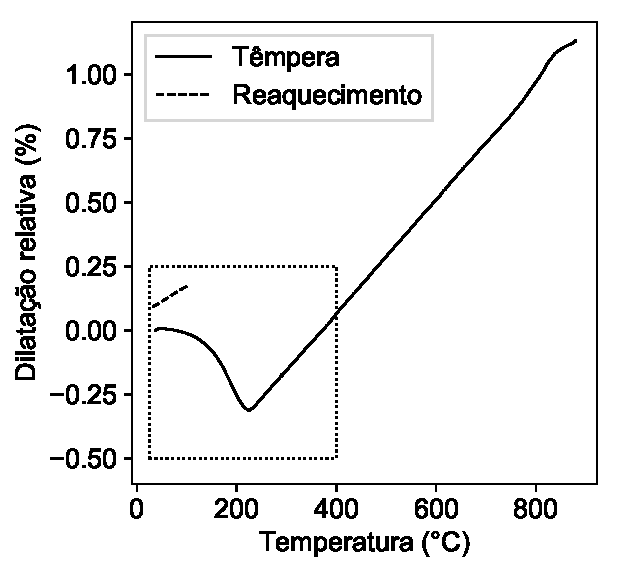
\includegraphics[width=.8\textwidth]{../tese/img/dilatometria/dil_martensita.pdf}
    \end{figure}
  }
  \only<2>{
    \begin{columns}
      \begin{column}{.6\textwidth}
        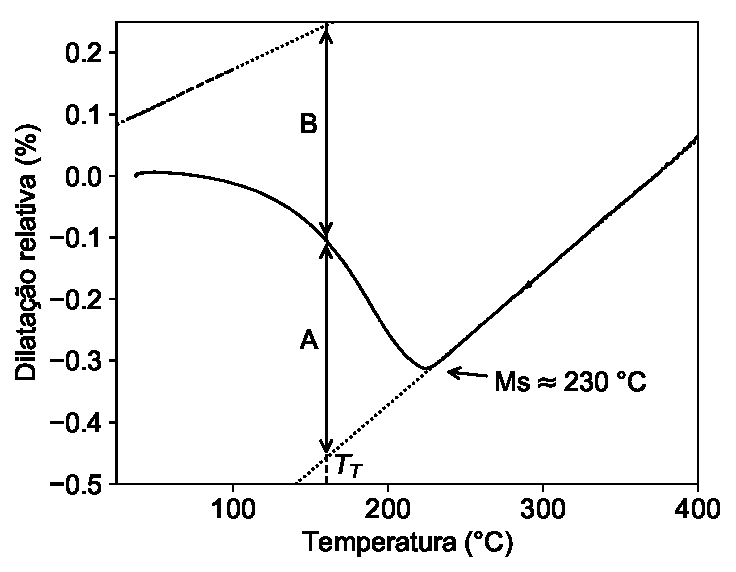
\includegraphics[width=\textwidth]{../tese/img/dilatometria/dil_martensita_close.pdf}
      \end{column}

      \begin{column}{.4\textwidth}
          Regra das alavancas:

          $$f^{\alpha'} = 1 - f^\gamma = \frac{A}{A + B}$$
      \end{column}
    \end{columns}
  }
\end{frame}

\begin{frame}{Transformação martensítica}
  $$f^{\alpha'} = 1 - f^\gamma = 1 - \exp\left[ -1,217 \times 10^{-2} \left( 216,2 - T_T \right) \right]$$

  \only<1>{
    \begin{figure}
      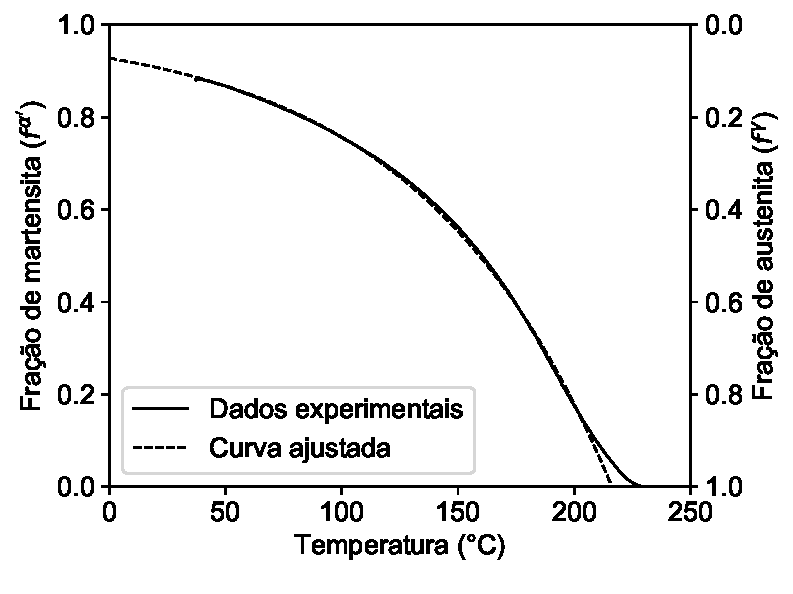
\includegraphics[width=.8\textwidth]{../tese/img/dilatometria/frac_martensita.pdf}
    \end{figure}
  }

  \only<2>{
    \begin{table}
      \begin{tabular}{c c c}
      \hline
      $T_T$ (°C) & $f^{\alpha'}$ (\% vol) & $f^\gamma$ (\% vol)\\
      \hline
      25 &  90,2 & 9,8\\
      140 & 60,4 & 39,6\\ 
      170 & 43,0 & 57,0\\
      200 & 17,9 & 82,1\\
      \hline
      \end{tabular}
    \end{table}
  }
\end{frame}

\begin{frame}{Transformação martensítica}
  $T_T = \SI{170}{\degreeCelsius} / \SI{1}{min}$ ($f^{\alpha'}$ = 43,0\%)

  \begin{figure}
    \includegraphics<1>[width=.8\textwidth]{img/TT170.pdf}
  \end{figure}
\end{frame}

\begin{frame}{Transformação martensítica}
  $T_T = \SI{170}{\degreeCelsius} / \SI{1}{min}$ ($f^{\alpha'}$ = 43,0\%)
  \begin{itemize}
    \item Martensita levemente revenida $\rightarrow$ atacada pelo Nital
    \item Áreas brancas / alto relevo: \textbf{austenita ($\gamma$)} não transformada após $\SI{170}{\degreeCelsius} / \SI{1}{min}$ $\rightarrow$ transforma-se parcialmente em \textbf{martensita fresca ($\alpha_{fr}'$)} durante resfriamento final
    \item \textbf{$\alpha_{fr}' + \gamma$: MA}
  \end{itemize}

  \begin{figure}
    \includegraphics<1>[width=.5\textwidth]{../tese/img/micrografias/Q170-1min/500x-1.pdf}
    \includegraphics<2>[width=.5\textwidth]{../tese/img/micrografias/Q170-1min/5kx-4_scalebar.pdf}
  \end{figure}
\end{frame}

\begin{frame}{Microssegregação}
  \begin{itemize}
    \item EPMA: composição medida de Mn, Si e Cu
    \item C calculado assumindo potencial químico homogêneo a 880~°C
  \end{itemize}

  \begin{figure}
    \includegraphics<1>[width=.7\textwidth]{../tese/img/EPMA/EPMA.pdf}
  \end{figure}
\end{frame}
  
% \begin{frame}{Microssegregação}
%   Simulação Scheil mostra mesma tendência de segregação

%   \begin{figure}
%     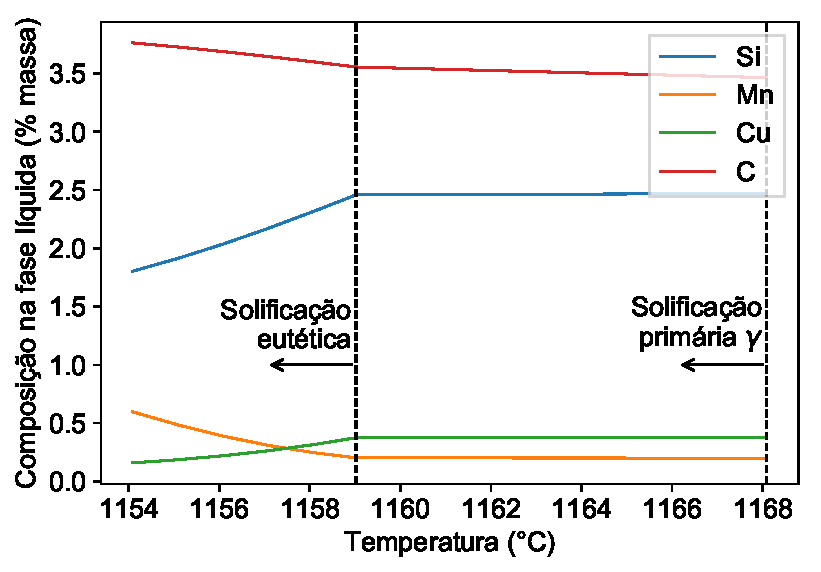
\includegraphics[width=.8\textwidth]{../tese/img/thermo-calc/scheil.pdf}
%   \end{figure}
% \end{frame}

\begin{frame}{Distribuição esperada da martensita}
  Ms calculado ponto a ponto:

  $$\textcolor{red}{Ms}\,\text{(°C)} = 565 - 600 \left[1 - \exp \left( -0.96 w_C^\gamma \right)\right] - 31 w_{Mn}^\gamma - 13 w_{Si}^\gamma$$

  A partir do Ms calculado, é determinada $f^{\alpha'}$ ponto a ponto pela equação de Koistinen-Marburger:

  $$f^{\alpha'} = 1 - \exp\left[ -1,217 \times 10^{-2} \left( \textcolor{red}{Ms} - T_T \right) \right]$$
\end{frame}

\begin{frame}{Distribuição esperada da martensita}
  $T_T = \SI{170}{\degreeCelsius}$

  \begin{figure}
    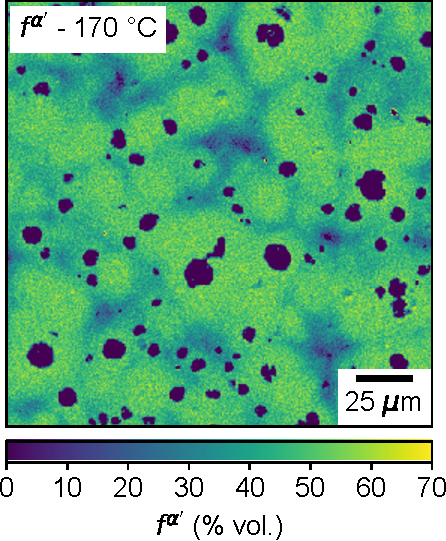
\includegraphics[width=.49\textwidth,valign=t]{img/fmart_TQ170.pdf}\hfill
    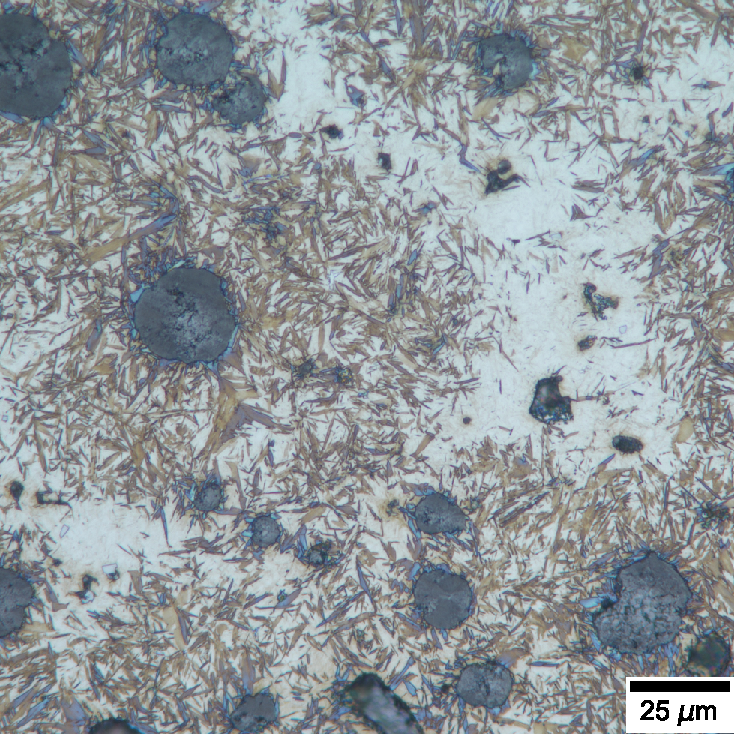
\includegraphics[width=.49\textwidth,valign=t]{../tese/img/micrografias/Q170-1min/500x-1.pdf}
  \end{figure}
\end{frame}

\begin{frame}{Distribuição esperada da martensita}
  \begin{itemize}
    \item $T_T = 25,\ 140,\ 170,\ \SI{200}{\degreeCelsius}$
    \item Histogramas da distribuição de $f^{\alpha'}$ calculada pelo método anterior
    \item Distribuição de martensita fica mais homogênea quanto a temperatura de têmpera é diminuída.
  \end{itemize}

  \begin{figure}
    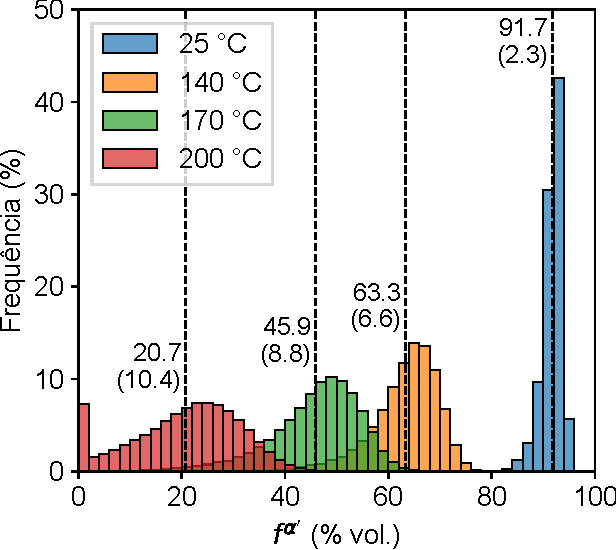
\includegraphics[width=.7\textwidth]{img/fmart_different_TQ.pdf}\hfill
  \end{figure}
\end{frame}

%%%%%%%%%%%%%%%%%%%%%%%%%%%%%%%%%%%%%%%%%%

\subsection{Caracterização microestrutural das amostras T\&P}

% \begin{frame}{Microestruturas T\&P}{Efeito do tempo de partição ($t_P$)}
%   $T_T = \SI{170}{\degreeCelsius}$; $T_P = \SI{375}{\degreeCelsius}$
  
%   \begin{itemize}
%     \item Áreas brancas: austenita não transformada na etapa de partição
%     \item<3> Tempos longos: austenita é consumida (bainita?)
%   \end{itemize}

%   \only<1>{
%     \begin{figure}
%       \subfloat[$t_P = 0$]{\includegraphics[width=.49\textwidth]{../tese/img/micrografias/170-375/MO/QP0_scalebar.pdf}}\hfill
%       \subfloat[$t_P = 30~s$]{\includegraphics[width=.49\textwidth]{../tese/img/micrografias/170-375/MO/QP30s_scalebar.pdf}}
%     \end{figure}
%   }
%   \only<2>{
%     \begin{figure}
%       \subfloat[$t_P = 0$]{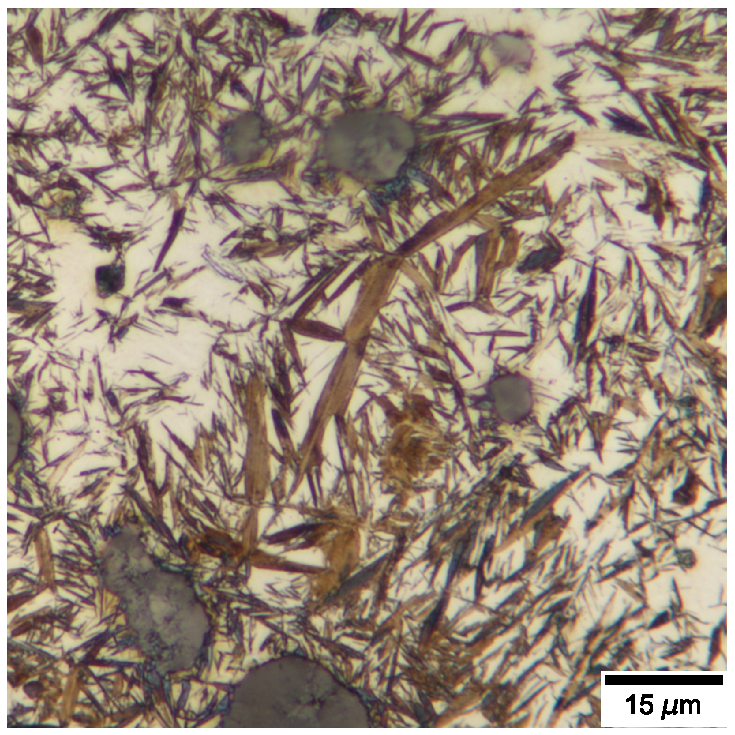
\includegraphics[width=.49\textwidth]{../tese/img/micrografias/170-375/MO/QP0_1000x_scalebar.pdf}}\hfill
%       \subfloat[$t_P = 30~s$]{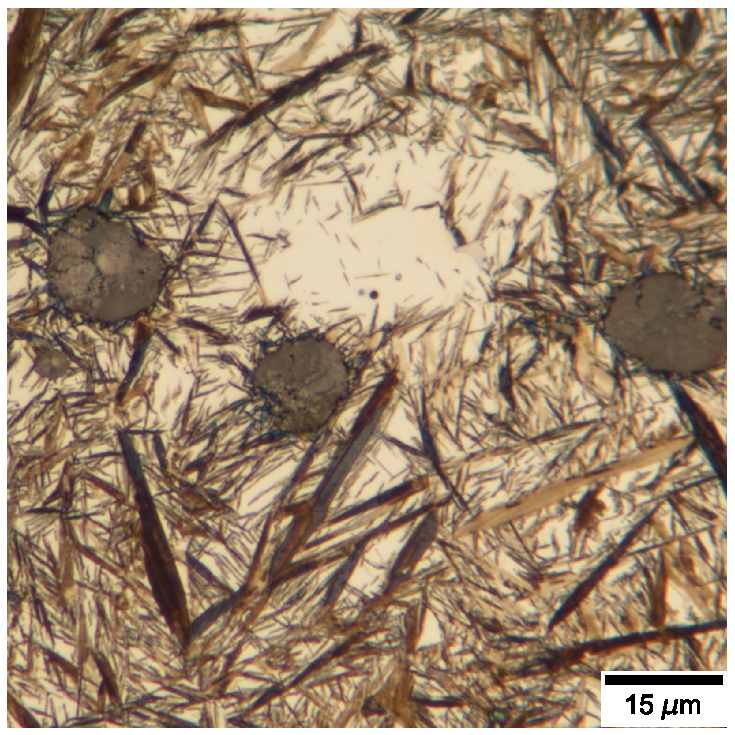
\includegraphics[width=.49\textwidth]{../tese/img/micrografias/170-375/MO/QP30s_1000x_scalebar.pdf}}
%     \end{figure}
%   }
%   \only<3>{
%     \begin{figure}
%       \subfloat[$t_P = 5~min$]{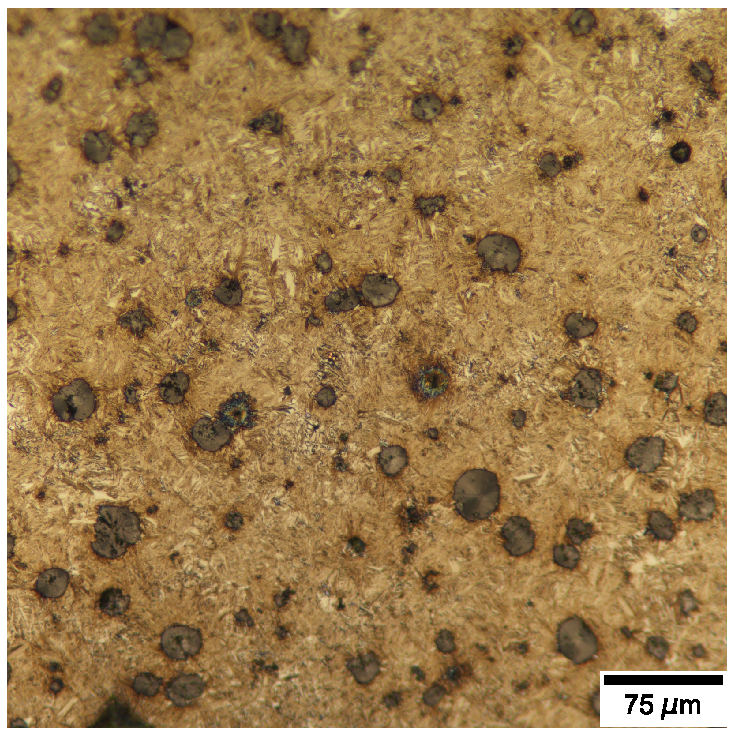
\includegraphics[width=.49\textwidth]{../tese/img/micrografias/170-375/MO/QP5min_scalebar.pdf}}\hfill
%       \subfloat[$t_P = 15~min$]{\includegraphics[width=.49\textwidth]{../tese/img/micrografias/170-375/MO/QP15min_scalebar.pdf}}
%     \end{figure}
%   }
% \end{frame}

\begin{frame}{Microestruturas T\&P}{Efeito do tempo de partição ($t_P$)}
  $T_T = \SI{170}{\degreeCelsius}$; $T_P = \SI{375}{\degreeCelsius}$ / 0

  \begin{itemize}
      % \item Áreas brancas em MO $\rightarrow$ alto relevo em MEV
      \item Padrão de ataque releva carbonetos ($\theta$) no tempo mais curto
      \item $\theta$ portanto se forma no aquecimento de $T_T$ a $T_P$
  \end{itemize}

  \begin{figure}
    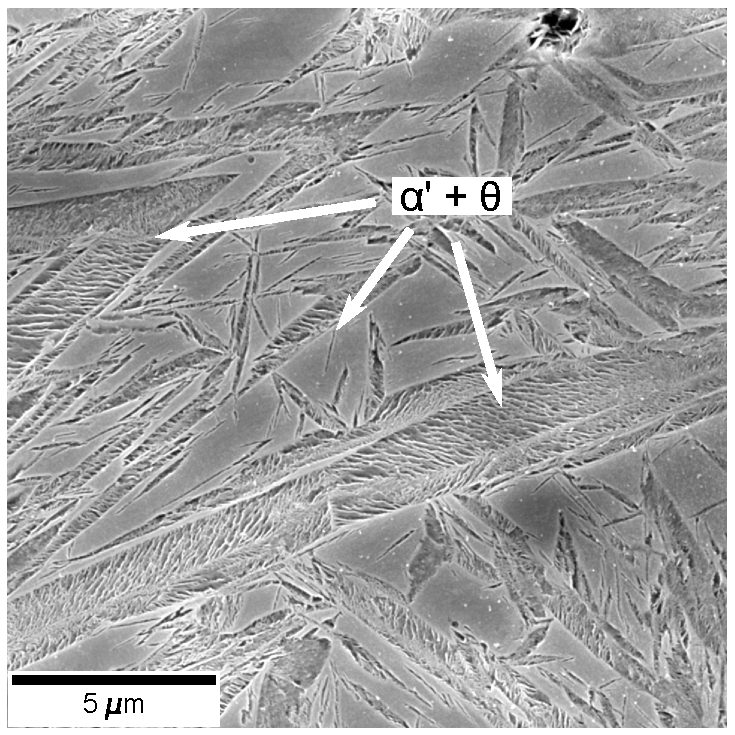
\includegraphics[width=.49\textwidth]{../tese/img/micrografias/170-375/MEV/0/5kx-3.pdf}\hfill
    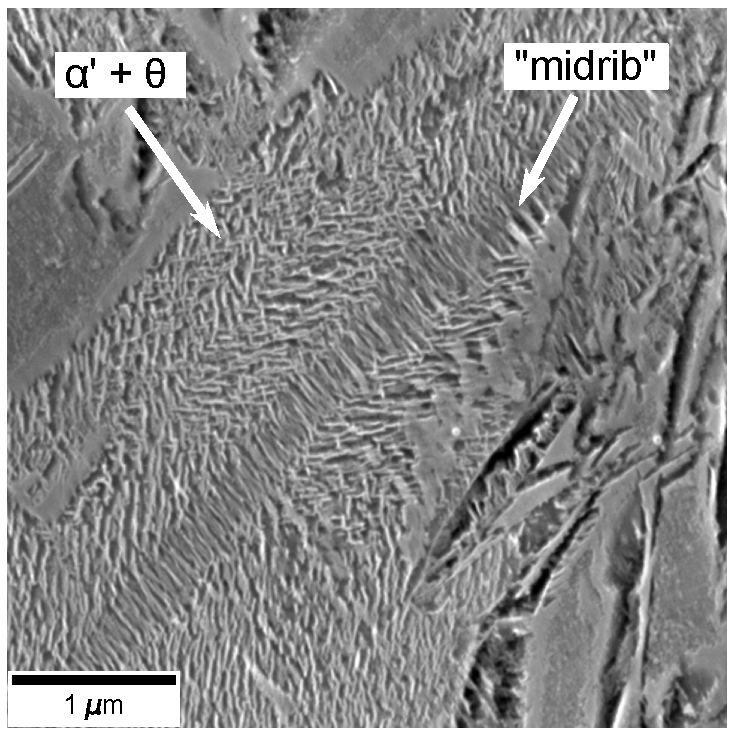
\includegraphics[width=.49\textwidth]{../tese/img/micrografias/170-375/MEV/0/20kx-1.pdf}
  \end{figure}
\end{frame}

\begin{frame}{Microestruturas T\&P}{Efeito do tempo de partição ($t_P$)}
  $T_T = \SI{170}{\degreeCelsius}$; $T_P = \SI{375}{\degreeCelsius}$ / \SI{30}{s}

  \begin{itemize}
      \item EBSD mostra \textbf{\color{green}austenita ($\gamma$) estabilizada}
      \item<2> Bainita não é acompanhada por carbonetos: \textbf{ferrita bainítica ($\alpha_b$)}
      \item<2> $\gamma$ próxima da martensita: evidência de partição!
  \end{itemize}

  \begin{figure}
    \includegraphics<1>[width=.49\textwidth]{../tese/img/micrografias/170-375/MEV/30s/5a.pdf}\hfill
    \includegraphics<1>[width=.49\textwidth]{../tese/img/micrografias/170-375/MEV/30s/5d.pdf}
    
    \includegraphics<2>[width=.49\textwidth]{../tese/img/micrografias/170-375/MEV/30s/5b.pdf}\hfill
    \includegraphics<2>[width=.49\textwidth]{../tese/img/micrografias/170-375/MEV/30s/5e.pdf}
  \end{figure}
\end{frame}

% \begin{frame}{Microestruturas T\&P}{Efeito do tempo de partição ($t_P$)}
%   $T_T = \SI{170}{\degreeCelsius}$; $T_P = \SI{375}{\degreeCelsius}$ / \SI{5}{min}
  
%   \begin{itemize}
%     \item $\alpha_b$ aumenta para tempos mais longos de partição
%     \item $\gamma$ fica mais homogeneamente distribuída
%   \end{itemize}

%   \begin{figure}
%     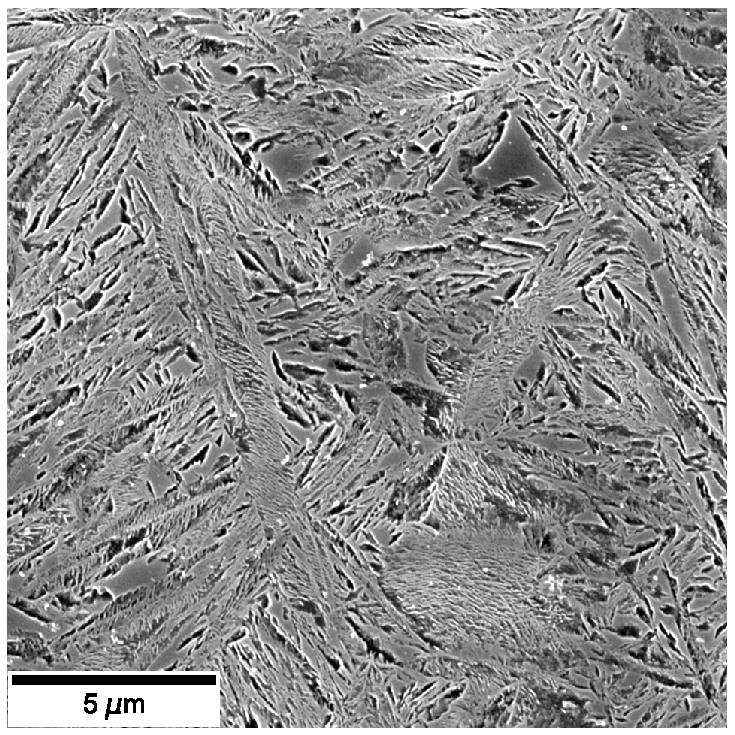
\includegraphics[width=.49\textwidth]{../tese/img/micrografias/170-375/MEV/5min/5kx-6.pdf}\hfill
%     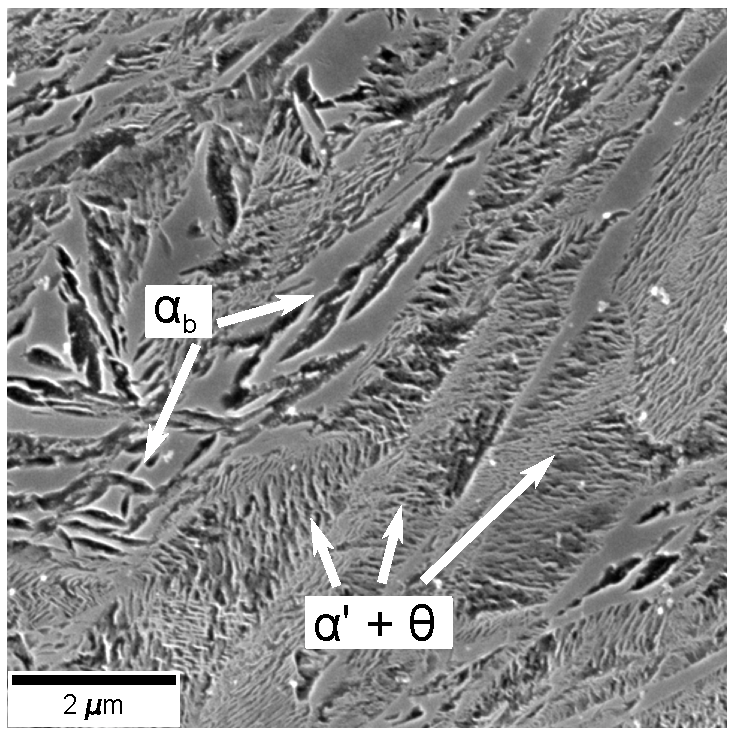
\includegraphics[width=.49\textwidth]{../tese/img/micrografias/170-375/MEV/5min/10kx-4.pdf}
%   \end{figure}
% \end{frame}

\begin{frame}{Microestruturas T\&P}{Efeito do tempo de partição ($t_P$)}
  $T_T = \SI{170}{\degreeCelsius}$; $T_P = \SI{375}{\degreeCelsius}$ / \SI{15}{min}
  
  \begin{figure}
    \includegraphics<1>[width=.49\textwidth]{../tese/img/micrografias/170-375/MEV/15min/1300x.pdf}\hfill
    \includegraphics<1>[width=.49\textwidth]{../tese/img/micrografias/170-375/MEV/15min/QP170-375-15_phase.pdf}
    
    \includegraphics<2>[width=.49\textwidth]{../tese/img/micrografias/170-375/MEV/15min/5kx-8.pdf}\hfill
    \includegraphics<2>[width=.49\textwidth]{../tese/img/micrografias/170-375/MEV/15min/5f.pdf}
  \end{figure}
\end{frame}

\begin{frame}{Microestruturas T\&P}{Efeito do tempo de partição ($t_P$)}
  $T_T = \SI{170}{\degreeCelsius}$; $T_P = \SI{375}{\degreeCelsius}$ / \SI{15}{min}
  
  EPMA
  
  \begin{figure}
    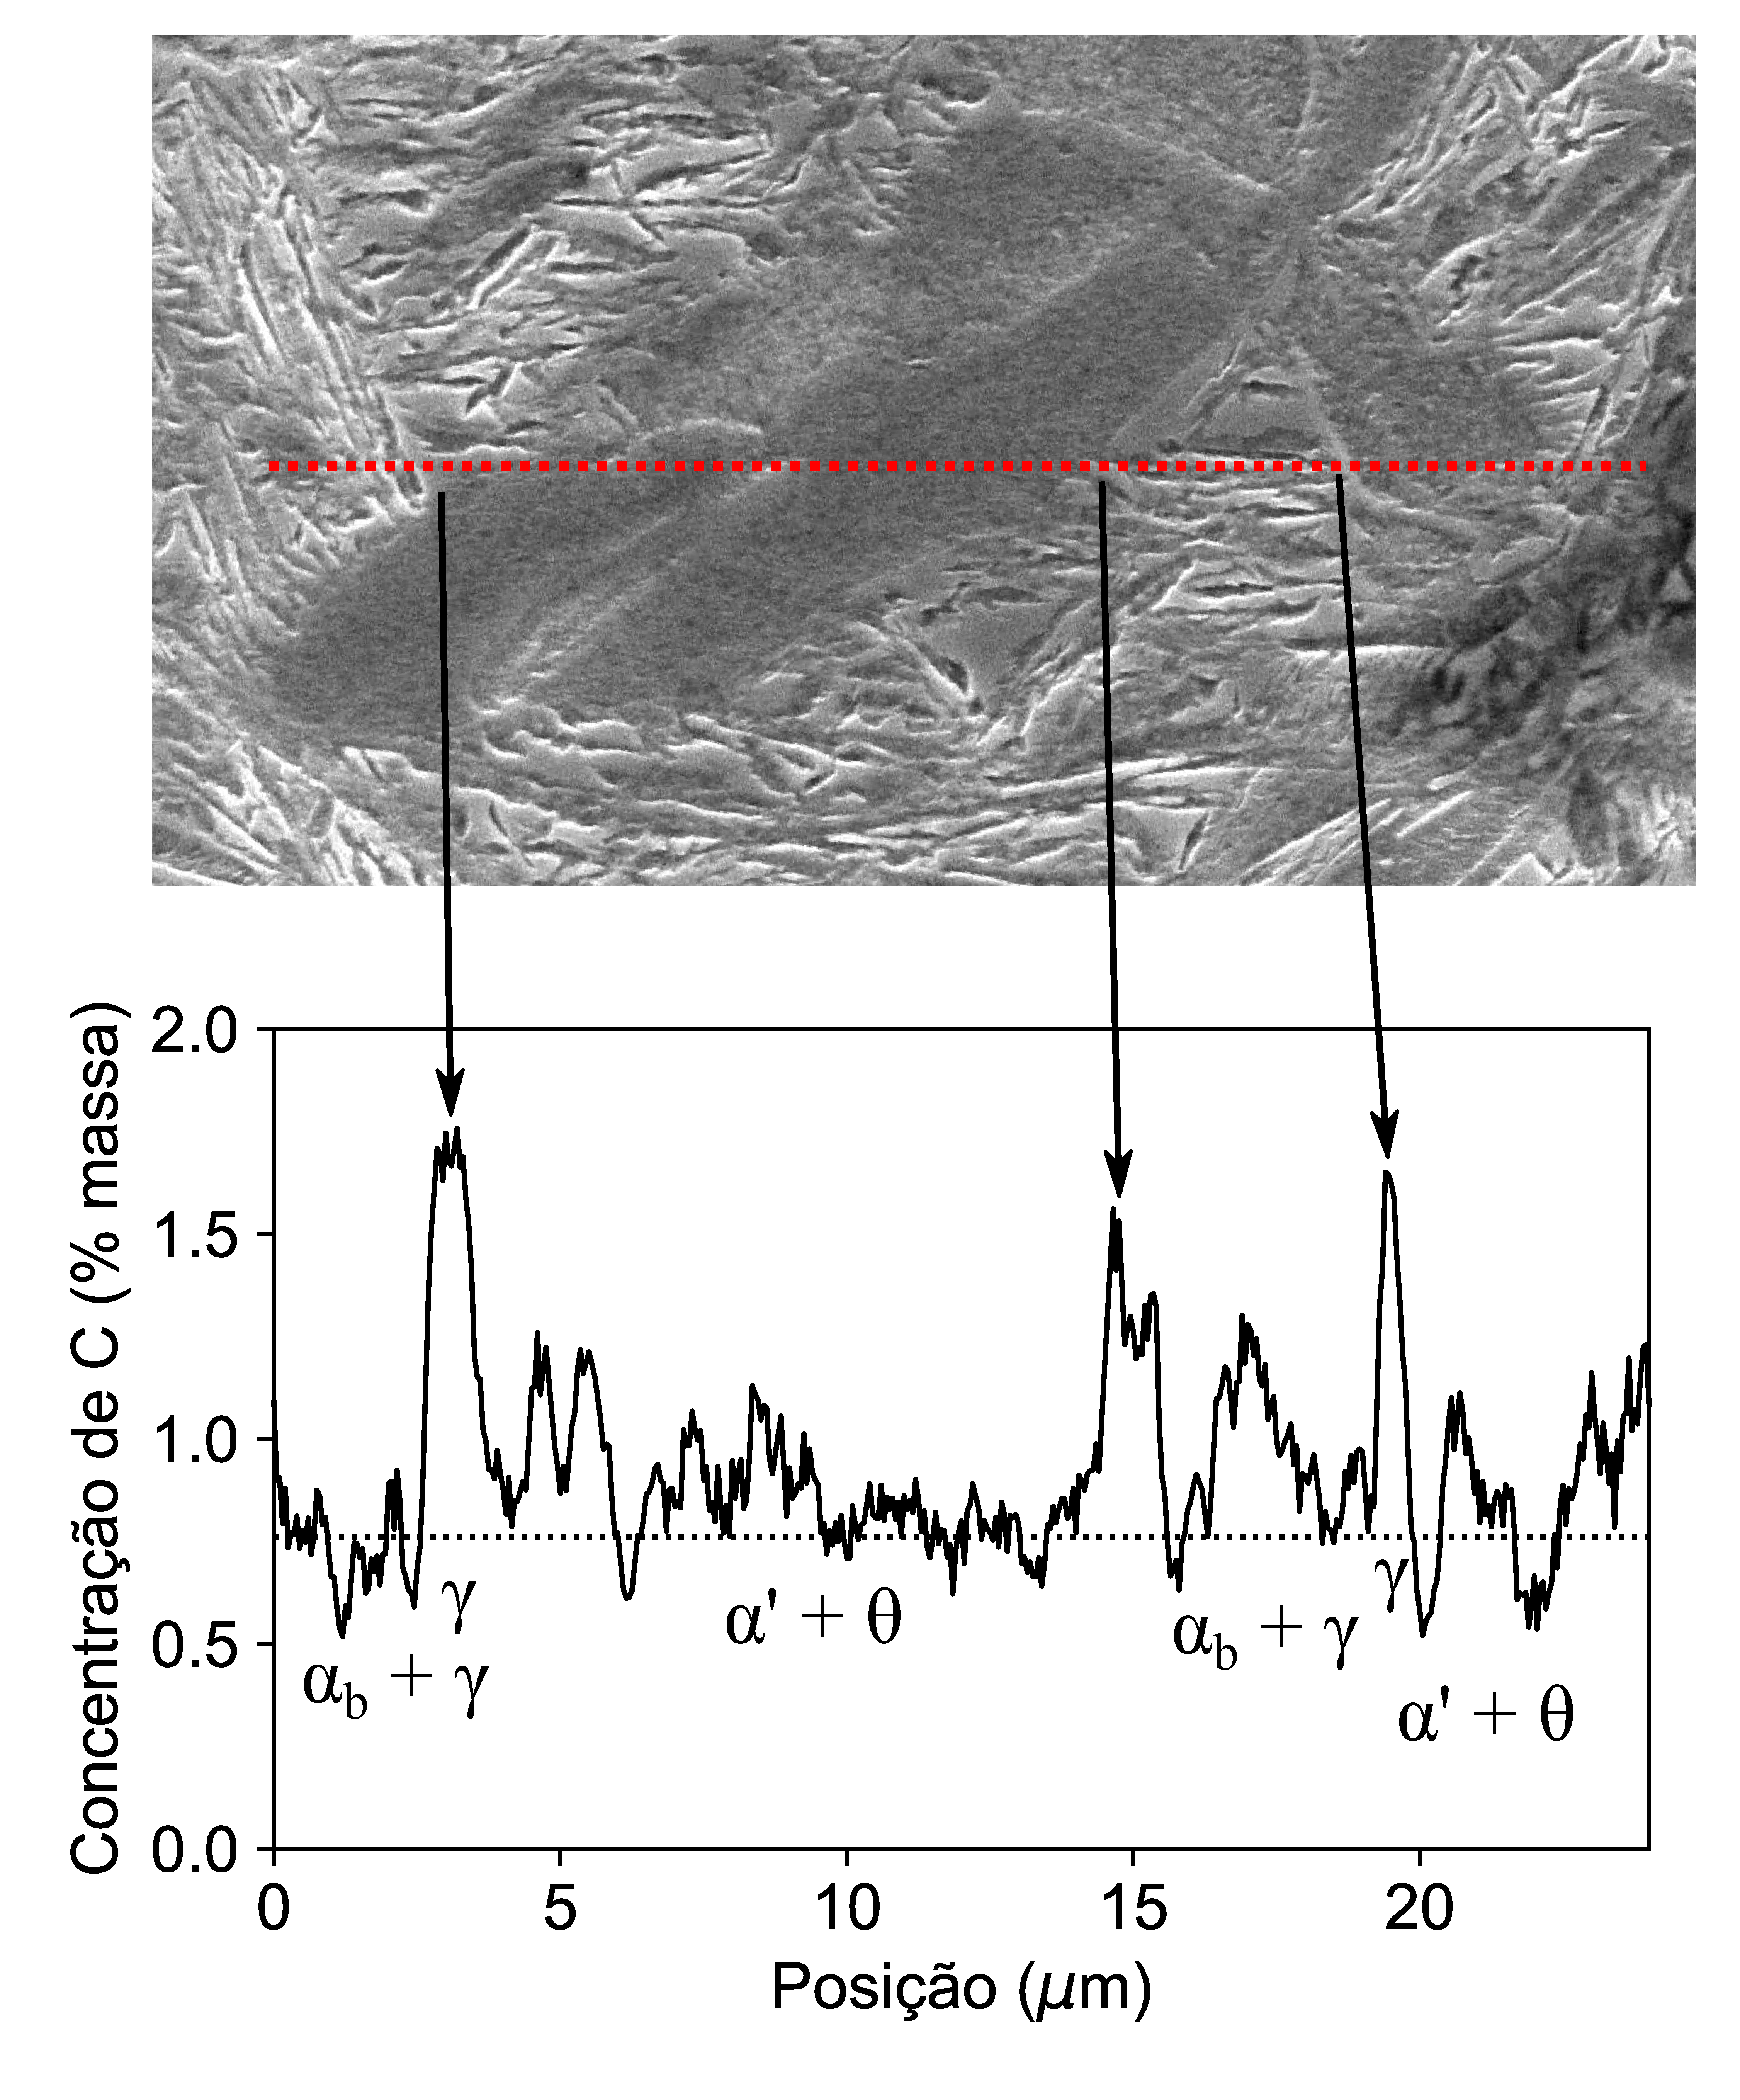
\includegraphics[width=.49\textwidth]{../tese/img/EPMA/0004LIN.pdf}\hfill
    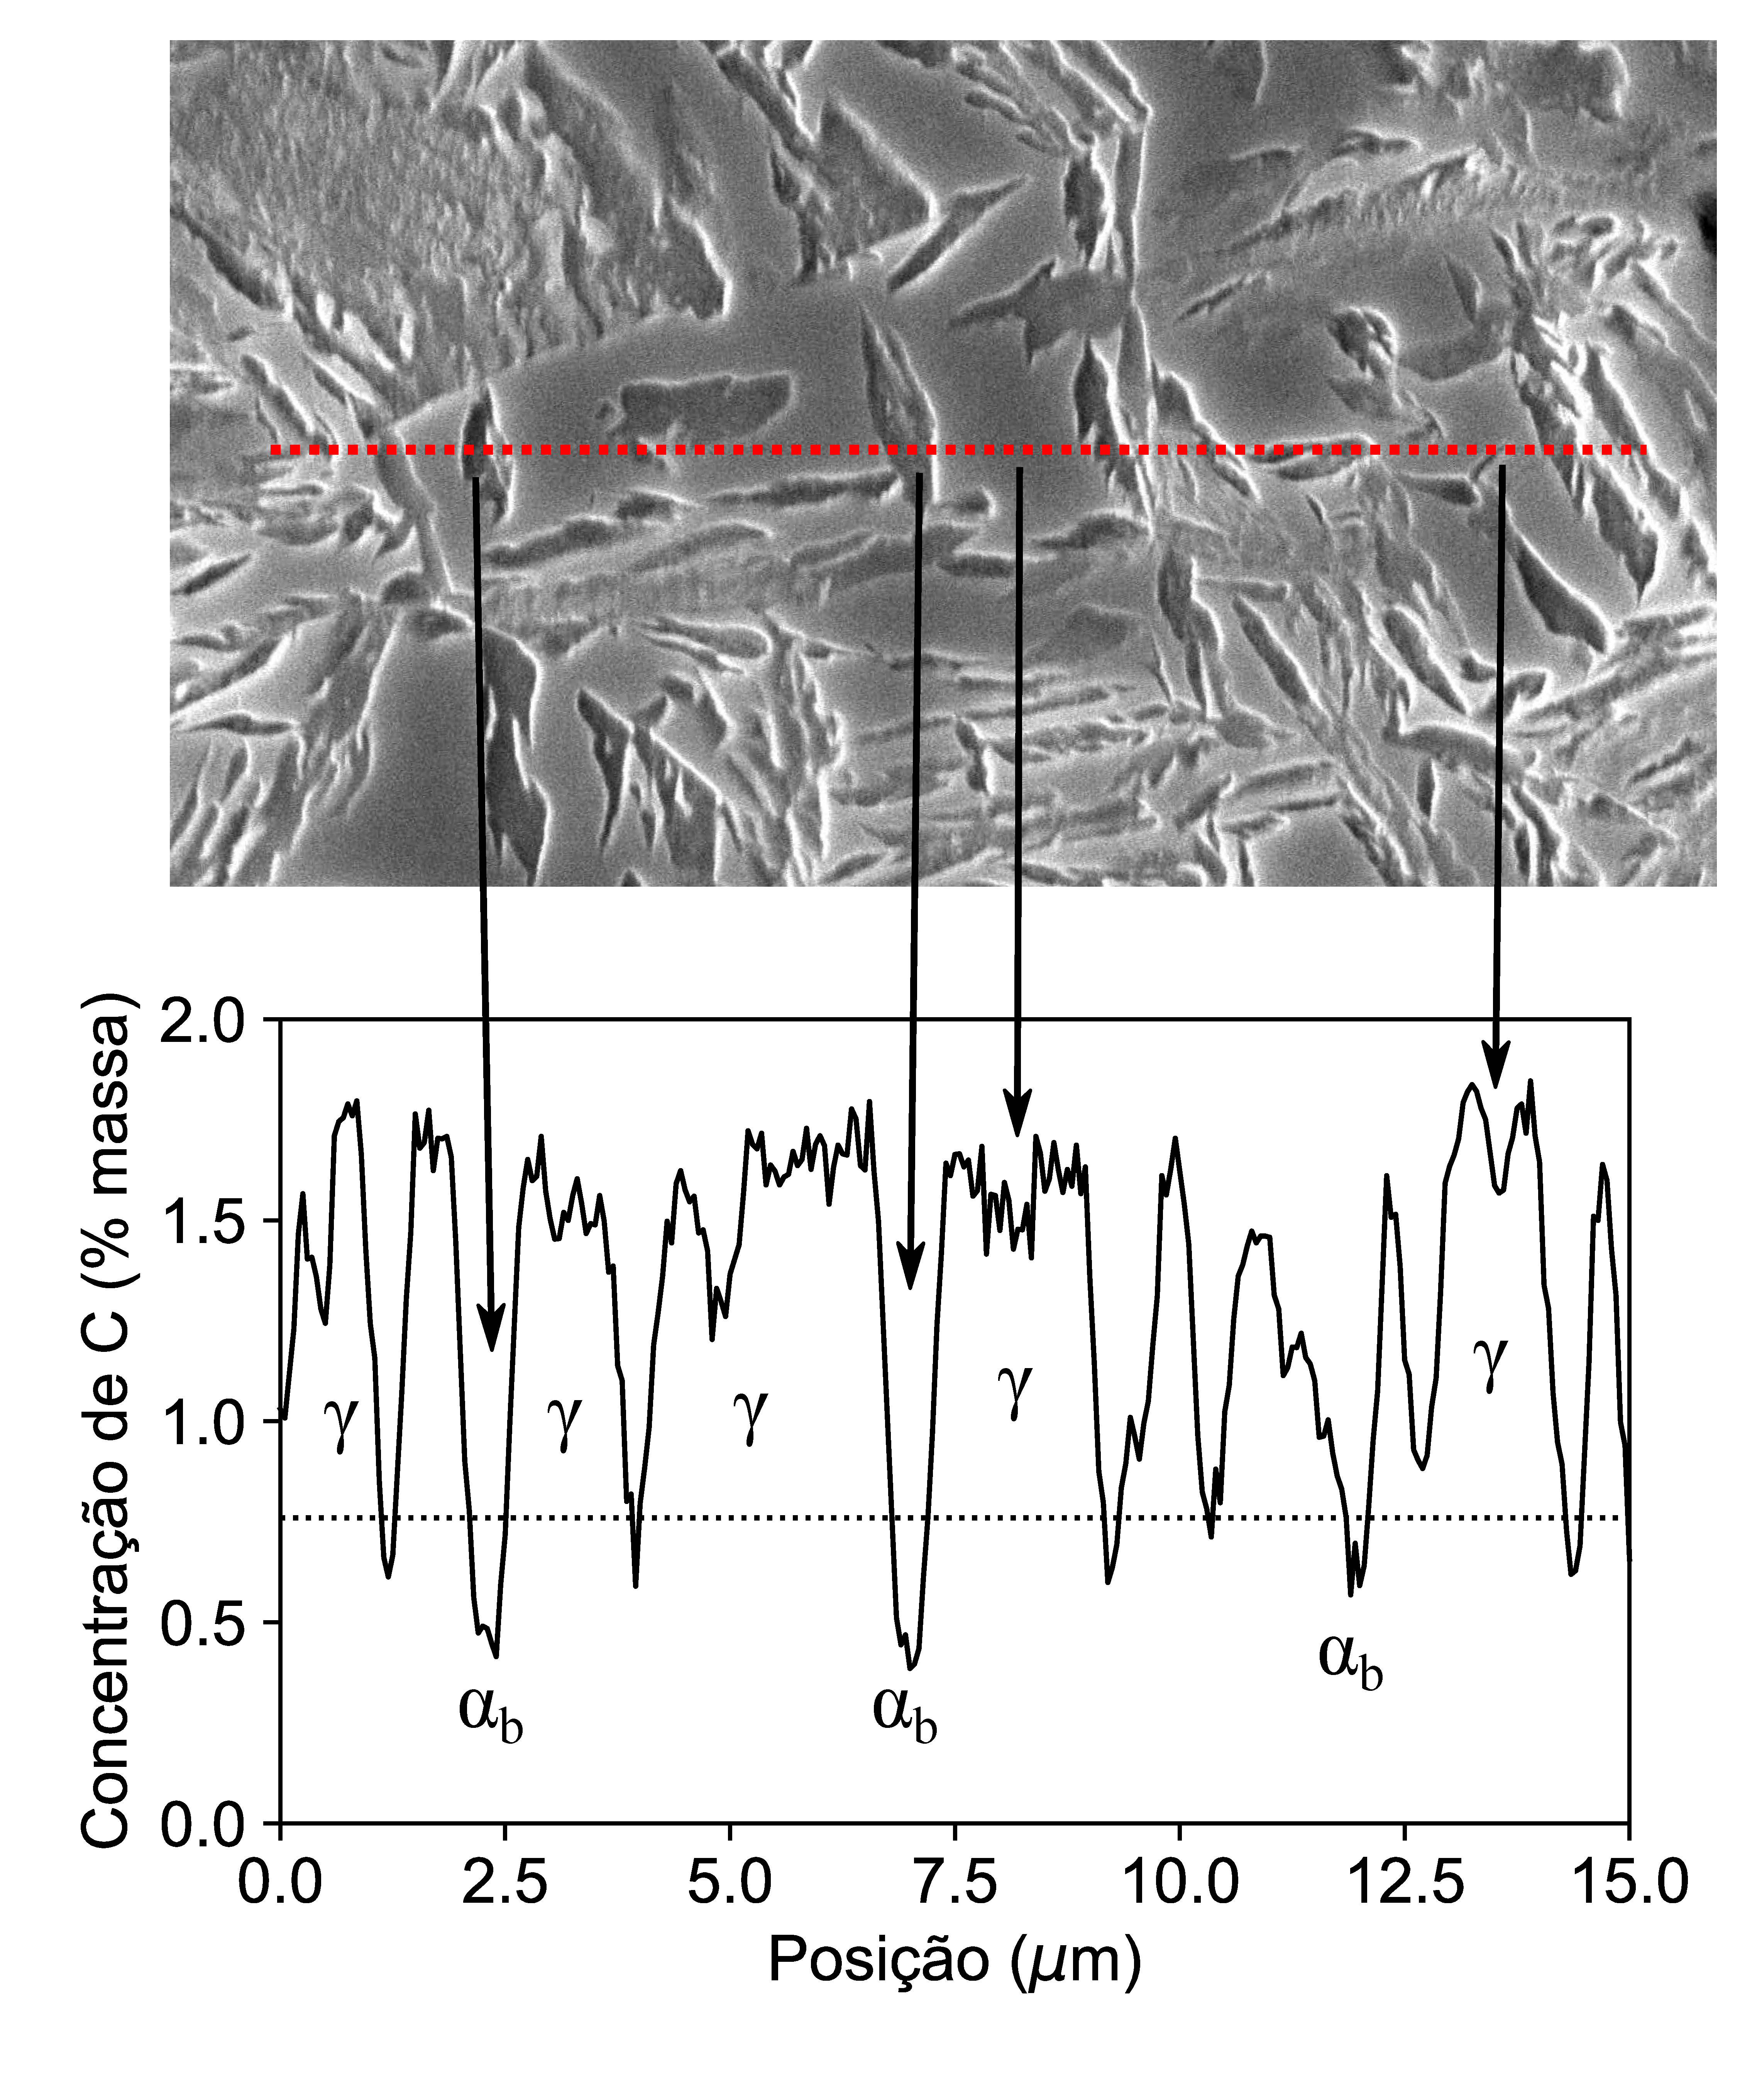
\includegraphics[width=.49\textwidth]{../tese/img/EPMA/0005LIN.pdf}
  \end{figure}
\end{frame}


%%%%%%%%%%%%%%%%%%%%%%%%

\begin{frame}{Microestruturas T\&P}{Efeito da temperatura de partição ($T_P$)}
  $T_T = \SI{170}{\degreeCelsius}$; $T_P = \SI{300}{\degreeCelsius}$ / \SI{15}{min}

  \begin{itemize}
    \item Carbonetos na martensita
    \item $\alpha_b$ mais refinada do que a \SI{375}{\degreeCelsius}
  \end{itemize}

  \begin{figure}
    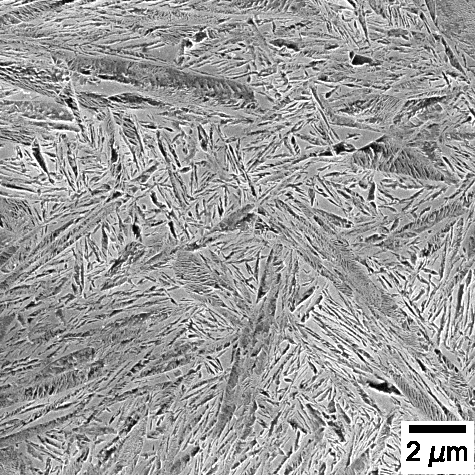
\includegraphics[width=.49\textwidth]{../tese/img/micrografias/170-outros/300C_5kx-3.pdf}\hfill
    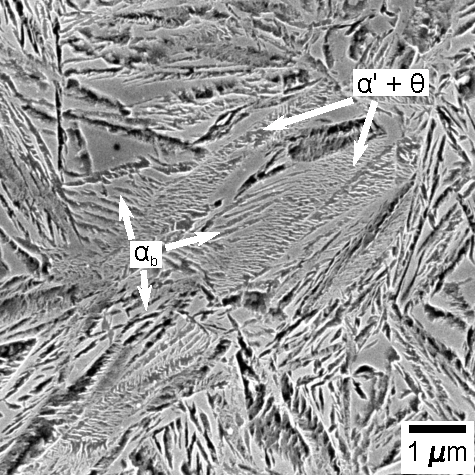
\includegraphics[width=.49\textwidth]{../tese/img/micrografias/170-outros/300C_10kx-1.pdf}
  \end{figure}
\end{frame}

\begin{frame}{Microestruturas T\&P}{Efeito da temperatura de partição ($T_P$)}
  $T_T = \SI{170}{\degreeCelsius}$; $T_P = \SI{450}{\degreeCelsius}$ / \SI{30}{s}

  \begin{itemize}
    \item Carbonetos na martensita
    \item $\alpha_b$ mais grossa do que a \SI{450}{\degreeCelsius}
    \item Nucleação de $\alpha_b$ nos contornos $\alpha' + \theta / \gamma$
  \end{itemize}

  \begin{figure}
    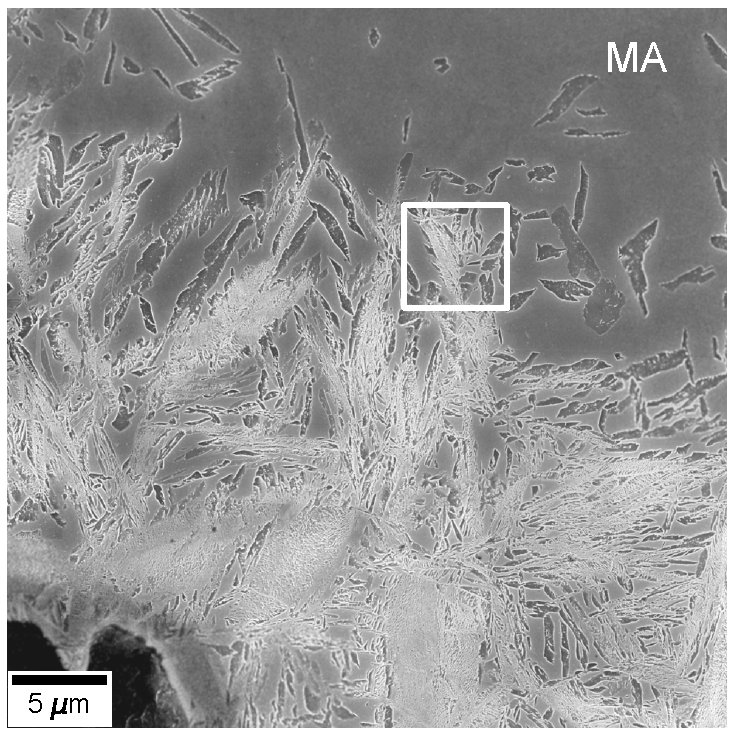
\includegraphics[width=.49\textwidth]{../tese/img/micrografias/170-outros/6b.pdf}\hfill
    % \includegraphics<1>[width=.49\textwidth]{../tese/img/micrografias/170-outros/6c.pdf}\\
    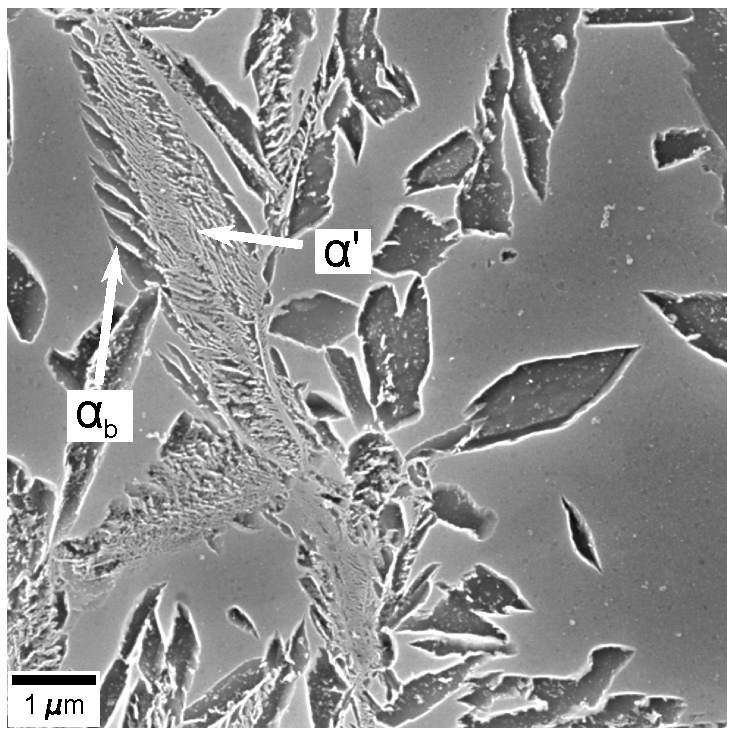
\includegraphics[width=.49\textwidth]{../tese/img/micrografias/170-outros/6d.pdf}
  \end{figure}
\end{frame}

\begin{frame}{Microestruturas T\&P}{Efeito da temperatura de partição ($T_P$)}
  $T_T = \SI{170}{\degreeCelsius}$; $T_P = \SI{450}{\degreeCelsius}$ / \SI{15}{min}

  \begin{itemize}
    \item Toda austenita é consumida após 15~min de partição
  \end{itemize}

  \begin{figure}
    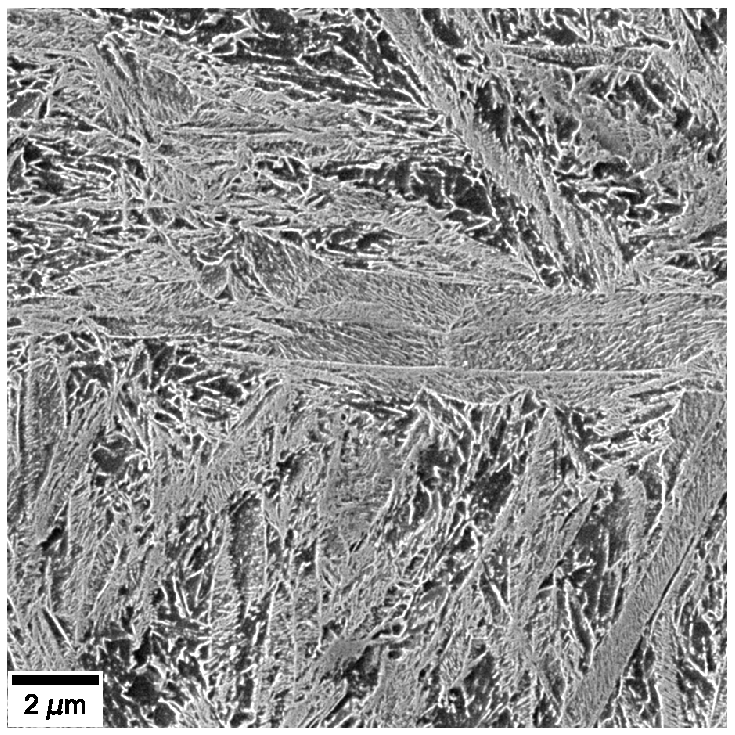
\includegraphics[width=.49\textwidth]{../tese/img/micrografias/170-outros/6e.pdf}\hfill
    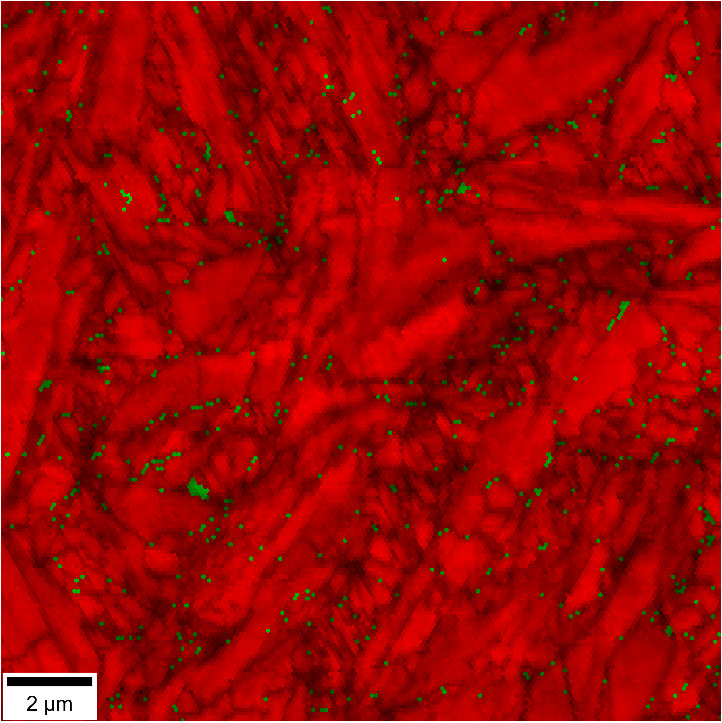
\includegraphics[width=.49\textwidth]{../tese/img/micrografias/170-outros/6f.pdf}
  \end{figure}
\end{frame}


%%%%%%%%%%%%%%%%%%%%%%%%

\begin{frame}{Microestruturas T\&P}{Efeito da temperatura de têmpera ($T_T$)}
  \begin{figure}
    \begin{itemize}
      \item $T_T$ = 140, 170 e \SI{200}{\degreeCelsius}; $T_P$ = \SI{300}{\degreeCelsius}
      \item Bainita é mais refinada quando menor $T_T$ (menores grãos não transformados de austenita)
    \end{itemize}

    \only<1>{\subfloat[$T_T=\SI{140}{\degreeCelsius}$]{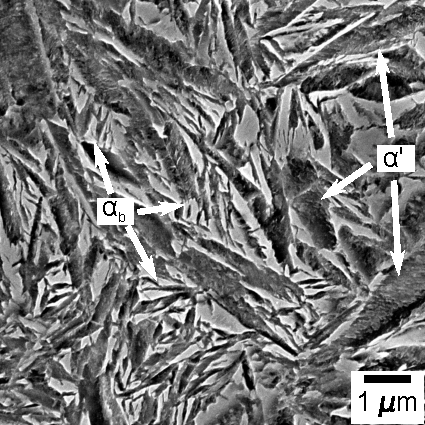
\includegraphics[width=.49\textwidth]{../tese/img/micrografias/efeito_tempera/140-300-2h.pdf}}\hfill}
    \only<1>{\subfloat[$T_T=\SI{170}{\degreeCelsius}$]{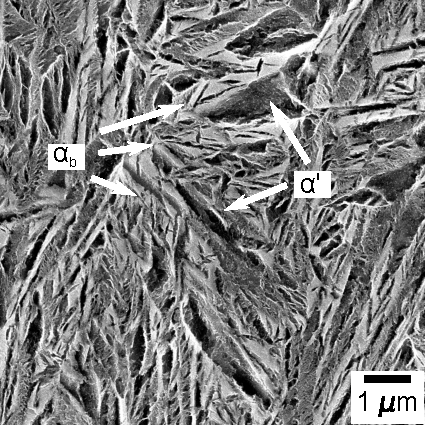
\includegraphics[width=.49\textwidth]{../tese/img/micrografias/efeito_tempera/170-300-2h.pdf}}}
    \only<2>{\subfloat[$T_T=\SI{200}{\degreeCelsius}$]{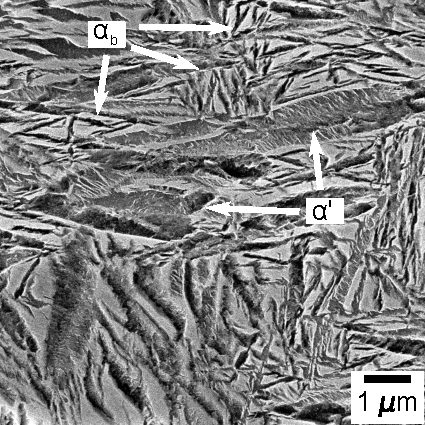
\includegraphics[width=.49\textwidth]{../tese/img/micrografias/efeito_tempera/200-300-2h.pdf}}}
  \end{figure}
\end{frame}

\begin{frame}{Microestruturas T\&P}{Efeito da temperatura de têmpera ($T_T$)}
  \begin{itemize}
    \item Efeito de refinamento da bainita mais claro pela observação da amostra austemperada a \SI{300}{\degreeCelsius}
  \end{itemize}

  \begin{figure}
    \includegraphics[width=.49\textwidth]{../tese/img/micrografias/ADI/300-15min/2500x-1.pdf}\hfill
    \includegraphics[width=.49\textwidth]{../tese/img/micrografias/ADI/300-15min/10kx-1.pdf}
  \end{figure}
\end{frame}

%%%%%%%%%%%%%%%%%%%%%%%%

\begin{frame}{Microestruturas T\&P}{Carbonetos}
  \begin{itemize}
    \item DRX síncrotron usando detector 2D
    \item $T_T = \SI{170}{\degreeCelsius}$
  \end{itemize}

  \begin{figure}
    \includegraphics<1>[width=\textwidth]{img/selected_diffractograms.pdf}
    \includegraphics<2>[width=\textwidth]{img/selected_diffractograms_detail.pdf}
  \end{figure}  
\end{frame}

\begin{frame}{Microestruturas T\&P}{Carbonetos}
  \begin{itemize}
    \item Cementita a \SI{450}{\degreeCelsius}
  \end{itemize}  

  \begin{figure}
    \includegraphics[width=\textwidth]{img/selected_diffractograms_cementite.pdf}
  \end{figure}
\end{frame}

\begin{frame}{Microestruturas T\&P}{Carbonetos}
  \begin{itemize}
    \item Carbonetos $\epsilon$ ou $\eta$ a 300 e \SI{375}{\degreeCelsius}
  \end{itemize}  

  \begin{figure}
    \includegraphics[width=.93\textwidth]{img/selected_diffractograms_eta.pdf}
  \end{figure}
\end{frame}

%%%%%%%%%%%%%%%%%%%%%%%%%%%%

\subsection{Cinética das transformações de fases durante T\&P}

\begin{frame}{Cinética}{Dilatometria}
  \begin{itemize}
    \item $T_T = \SI{170}{\degreeCelsius}$
    \item Dilatação durante a etapa de partição: expansão em todas as condições
    \item Contração a \SI{450}{\degreeCelsius}: cementita
  \end{itemize}

  \begin{figure}
    \includegraphics[width=.8\textwidth]{../tese/img/dilatometria/dlxt_QT=170-PT.pdf}
    % \includegraphics<2>[width=.8\textwidth]{../tese/img/dilatometria/dil_extra.pdf}
  \end{figure}
\end{frame}

\begin{frame}{Cinética}{Dilatometria}
  \begin{itemize}
    \item Austêmpera (sem martensita): expansão ocorre mais lentamente; tempo de incubação
    \item<2> $T_P = \SI{300}{\degreeCelsius}$, variando $T_T$
  \end{itemize}

  \begin{figure}
    \includegraphics<1>[width=.8\textwidth]{../tese/img/dilatometria/dlxt_austempera.pdf}
    \includegraphics<2>[width=.8\textwidth]{../tese/img/dilatometria/dlxt_PT300.pdf}
  \end{figure}
\end{frame}

\begin{frame}{Cinética}{Dilatometria}
  \begin{itemize}
    \item Presença da martensita afeta a cinética da reação bainítica
    \item Como mostra micrografias, nucleação de $\alpha_b$ ocorre nas interfaces $\alpha'/\theta$
  \end{itemize}
\end{frame}

% \begin{frame}{Cinética}{Dilatometria}
%   \begin{itemize}
%     \item $T_T = \SI{170}{\degreeCelsius}$
%     \item Dilatação $\times$ temperatura
%     \item<1> $t_P = 2~h$: Desvio da dilatação esperada $\rightarrow$ reação bainítica começa antes de $T_P$ ser atingido
%     \item<2> $t_P = 30~s$: Formação de $\alpha'_{fr}$ no resfriamento final
%   \end{itemize}

%   \begin{figure}
%     \includegraphics<1>[width=.8\textwidth]{../tese/img/dilatometria/dlxT_qPT2h_fc.pdf}
%     \includegraphics<2>[width=.8\textwidth]{../tese/img/dilatometria/dlxT_qPT30s-fc.pdf}
%   \end{figure}
% \end{frame}

%%%%%%%%%%%%%%%%%%%%%%%%%%%%%%%%%% DRX in situ

\begin{frame}{Cinética}{Difração de raios X \textit{in situ}}
  \begin{itemize}
    % \item $T_T = \SI{170}{\degreeCelsius}$; $T_P = \SI{300}{\degreeCelsius} / 2~h$; 
    % \item Eixo X: $2\theta$; eixo Y: Tempo de partição [s]
    \item Evolução do pico (111)$\gamma$: atenuação e deslocamento para maiores valores de distância interplanar $\rightarrow$ Reação bainítica consome $\gamma$; carbono distorce $\gamma$
  \end{itemize}

  \begin{figure}
    \includegraphics[width=.8\textwidth]<1>{../tese/img/XTMS/XTMS_colormap_full.pdf}
    \includegraphics[width=.8\textwidth]<2>{../tese/img/XTMS/XTMS_colormap_detail.pdf}
  \end{figure}
\end{frame}

\begin{frame}{Cinética}{Difração de raios X \textit{in situ}}
  \begin{itemize}
    \item $T_T = \SI{170}{\degreeCelsius}$
    \item Fração de ferrita bainítica $f^{\alpha_b}$ calculada assumindo que $f^{\alpha'}$ é constante
    \item A \SI{450}{\degreeCelsius} toda $\gamma$ é consumida
    \item<2> $f^{\alpha_b}$ para $t_P = 0$ é maior do que zero $\rightarrow$ $\alpha_b$ no aquecimento
  \end{itemize}

  \begin{figure}
    \includegraphics<1>[width=.85\textwidth]{../tese/img/XTMS/XTMS_ph_fraction.pdf}
    \includegraphics<2>[width=.85\textwidth]{../tese/img/XTMS/XTMS_ph_fraction_detail.pdf}
  \end{figure}
\end{frame}

\begin{frame}{Cinética}{Difração de raios X \textit{in situ}}
  \begin{itemize}
    \item Em todas condições $\gamma$ enriquece em carbono
    \item Tendências parecem com as curvas de $f^{\alpha_b}$
    \item Sugere que enriquecimento em C de $\gamma$ é controlado por formação de $\alpha_b$
  \end{itemize}

  \begin{figure}
    \centering
    \includegraphics<1>[width=.8\textwidth]{../tese/img/XTMS/XTMS_wC.pdf}
    \includegraphics<2>[width=.8\textwidth]{../tese/img/XTMS/XTMS_wC_detail.pdf}
  \end{figure}
\end{frame}

\begin{frame}
  \begin{itemize}
    \item Limite termodinâmico da partição de carbono
    \item Toji, Miyamoto e Raabe (2015)\footnotemark[1] observaram experimentalmente a partição de carbono entre $(\alpha' + \theta)$ e $\gamma$ mesmo na presença de $\theta$ precipitado em $\alpha'$
    \item<2> Partição de carbono é possível se $\mu_C^{\alpha' + \theta} > \mu_C^\gamma$
    \item<2> Modelo ECC$\theta$ (CCE$\theta$) de Toji: carbono em $\gamma$ ($w_C^\gamma$) após partição na presença de $\theta$
    \item<2> $w_C^\gamma$ depende da energia livre de $\theta$, mas não de $f^{\alpha'}$
  \end{itemize}

  \begin{figure}
    \includegraphics<1>[width=\textwidth]{img/toji_2015.pdf}
    \includegraphics<2>[width=.7\textwidth]{../tese/img/common_tangent.pdf}
  \end{figure}

  \footnotetext[1]{Toji, Y., Miyamoto, G. \& Raabe, D. Carbon partitioning during quenching and partitioning heat treatment accompanied by carbide precipitation. Acta Mater. 86, 137–147 (2015).}
\end{frame}

\begin{frame}
  \begin{itemize}
    \item ECC$\theta$ na liga estudada para diferentes carbonetos
    \item Extremos: ortocementita (mais estável, partição de elementos substitucionais) e paracementita (cementita de paraequilíbrio)
  \end{itemize}

  \begin{figure}
    \includegraphics[width=.8\textwidth]{../tese/img/thermo-calc/CCE.pdf}
  \end{figure}
\end{frame}

\begin{frame}
  \begin{itemize}
    \item Limite termodinâmico da reação bainítica
    \item Pela teoria difusional: paraequilíbrio; pela teoria sem difusão: $T_0$ ou $T_0'$
    \item Paraequilíbrio não descreve bem resultados experimentais
    \item Modelo WBs Hillert\footnotemark[1]: força motriz adicional calculada a partir de dados empíricos
  \end{itemize}

  \begin{figure}
    \includegraphics[width=.8\textwidth]{../tese/img/thermo-calc/WBs_para.pdf}
  \end{figure}

  \footnotetext[1]{Hillert, M., Höglund, L. \& Ågren, J. Escape of carbon from ferrite plates in austenite. Acta Metall. Mater. 41, 1951–1957 (1993).}
\end{frame}


\begin{frame}{Resumo dos resultados experimentais}
  \begin{itemize}
    \item Segregação causa distribuição heterogênea de $\alpha'$: regiões próximas de contornos de célula apresentam menos $\alpha'$
    \item Carbonetos precipitam em $\alpha'$ durante o aquecimento de $T_T$ a $T_P$
    \item Partição de carbono entre $\alpha + \theta$ e $\gamma$ acontece para curtos tempos
    \item Carbonetos não são completamente dissolvidos durante partição
    \item Reação bainítica acontece durante a etapa de partição
    \item Curvas de $f^{\alpha_b}$ e $w_C^\gamma$ e modelo WBs sugerem que enriquecimento em C de $\gamma$ é controlado por formação de $\alpha_b$
  \end{itemize}
\end{frame}


%%%%%%%%%%%%%%%%%%%%%%%%%%%%%%


\subsection{Modelo computacional de redistribuição de carbono}

\begin{frame}{Modelo redistribuição de C}
  Hipótese: poderia o \textit{soft impingement} (interação dos perfis de difusão) desacelerar a partição de carbono entre $\alpha'$ ($\alpha' + \theta$) e $\gamma$?

  \begin{figure}
    \includegraphics[width=.8\textwidth]{img/C_profiles.pdf}
  \end{figure}

  Simulações computacionais: crescimento $\alpha_b$ e partição de carbono entre $\alpha' + \theta$ e $\gamma$
\end{frame}

\begin{frame}{Modelo redistribuição de C}{Metodologia}
  % Na literatura: Mujahid e Bhadeshia, 1992; Hillert et al, 1992; Santofimia et al., 2008, 2009: partição de carbono entre placa supersaturada em carbono de ferrita e austenita
  % It consists of a mixed-model assuming both Zener's theory of diffusional transformations and Christian's theory of interface controlled phase transformations

  \begin{itemize}
    \item Apenas partição de carbono (paraequilíbrio)

    \item Igualdade dos potenciais químicos de C na interface

    \item Fluxos de carbono são balanceados pelo problema de Stefan:
    
    $$-D_C^\alpha \frac{d c^\alpha}{d z}\Bigg|_{int} + v\left(c^\gamma_{int} - c^\alpha_{int} \right) = -D_C^\gamma \frac{d c^\gamma}{d z}\Bigg|_{int}$$

    \item Interfaces $(\alpha' + \theta)/\gamma$ são fixas ($v = 0$)

    \item Interfaces $\alpha_b/\gamma$ são móveis. Velocidade é contabilizada pelo modelo de modo misto ($v = \frac{M}{V_m} \Delta G_{quim}$)

    \item Dados termodinâmicos (potenciais químicos) obtidos usando Thermo-Calc (TCFE8)

    \item Segunda lei de Fick resolvida numericamente utilizando o método de diferenças finitas
    
    $$ \frac{\partial c}{\partial t} = \frac{\partial}{\partial z} \left( D \frac{\partial c}{\partial z} \right) $$
  \end{itemize}
\end{frame}

\begin{frame}{Modelo redistribuição de C}
  Resultados divididos em duas partes:

  \begin{itemize}
    \item Sem bainita + efeito da precipitação de carbonetos com diferentes energias livres
    \item Com bainita + efeito da precipitação de carbonetos com diferentes energias livres
  \end{itemize}
\end{frame}

\begin{frame}{Partição de carbono $(\alpha' + \theta)/\gamma$}
  \begin{itemize}
    \item Simulações sem bainita
    \item Quando considerados, carbonetos estão presentes desde $t_P = 0$
    \item Composição interfacial em $\gamma$ determinado pelo modelo ECC$\theta$
    \item Geometria equivalente a T\&P com $T_T = \SI{170}{\degreeCelsius}$ ($f^{\alpha'} = 43\%$) e $T_P = \SI{375}{\degreeCelsius}$
    \item Largura das regiões das fases: $\alpha'$ \SI{1.0}{\mu m}; $\gamma$ \SI{1.32}{\mu m}
  \end{itemize}

  \begin{figure}
    \includegraphics[width=.8\textwidth]{img/simulations_nobainite.pdf}
  \end{figure}
\end{frame}

\begin{frame}{Partição de carbono $\alpha'/\gamma$}
  Sem carbonetos

  \begin{itemize}
    \item Caso mais simples de todos
    \item C em $\gamma$ na interface cresce rapidamente (max. $\approx$~4,5\%)
    \item Partição muito rápida: todo C em $\alpha'$ difunde para austenita em cerca de 1~s
  \end{itemize}

  \begin{figure}
    \includegraphics[width=.55\textwidth]{../tese/img/cpartition/cprofiles/mart_FoFo_CCE.pdf}
  \end{figure}
\end{frame}

\begin{frame}{Partição de carbono $(\alpha' + \theta)/\gamma$}
  $\theta$: Ortocementita

  \begin{itemize}
    \item $\mu_C^{\alpha' + \theta} < \mu_C^\gamma \rightarrow$ Carbono interfacial em $\gamma$ calculado pelo ECC$\theta$ é \emph{menor do que $c_0$}
    \item Difusão de carbono acontece de $\gamma$ para $\alpha' + \theta$
    \item \emph{Aumento de carbono em $\alpha' + \theta \rightarrow$ aumento da fração de carbonetos}
  \end{itemize}

  \begin{figure}
    \includegraphics<1>[width=.55\textwidth]{../tese/img/cpartition/cprofiles/mart_FoFo_CCEortho.pdf}
    % \includegraphics<2>[width=.55\textwidth]{../tese/img/cpartition/muprofiles/mart_FoFo_CCEortho.pdf}
  \end{figure}
\end{frame}

\begin{frame}{Partição de carbono $(\alpha' + \theta)/\gamma$}
  $\theta$: Paracementita

  \begin{itemize}
    \item Paracementita: carboneto de alta energia livre (interação negativa Si-C aumenta atividade de C)
    \item $\mu_C^{\alpha' + \theta} > \mu_C^\gamma \rightarrow$ partição ocorre de $\alpha' + \theta$ para $\gamma$
    \item \emph{Diminuição de carbono em $\alpha' + \theta \rightarrow$ diminuição da fração de carbonetos}
    \item Partição é mais lenta do que no cenário sem carbonetos
  \end{itemize}

  \begin{figure}
    \includegraphics<1>[width=.55\textwidth]{../tese/img/cpartition/cprofiles/mart_FoFo_CCEpara.pdf}
    % \includegraphics<2>[width=.55\textwidth]{../tese/img/cpartition/muprofiles/mart_FoFo_CCEpara.pdf}
  \end{figure}
\end{frame}

\begin{frame}{Partição de carbono $(\alpha' + \theta)/\gamma$}
  \begin{itemize}
    \item Nem ortocementita nem paracementita devem representar bem carbonetos de transição
    \item Dados termodinâmicos de carbonetos de transição não são encontrados na literatura
    \item Simulações feitas para carbonetos com energias livres variando de ortocementita para paracementita
  \end{itemize}

  \begin{figure}
    \includegraphics[width=.7\textwidth]{../tese/img/thermo-calc/CCE.pdf}
  \end{figure}
\end{frame}

\begin{frame}{Partição de carbono $(\alpha' + \theta)/\gamma$}
    \begin{itemize}
      \item Energias livres representadas pelo potencial químico $\mu_C^{\alpha' + \theta}$
      \item Partição é mais lenta quando os carbonetos possuem menor energia livre (mais estáveis)
      \item $\theta$ mais estável $\rightarrow$ menor carbono interfacial em $\gamma$ $\rightarrow$ difusão de C mais lenta
    \end{itemize}

  \begin{figure}
    \includegraphics[width=.8\textwidth]{../tese/img/cpartition/nobainite_cavg.pdf}
  \end{figure}
\end{frame}

%%%%%%% Com bainita

\begin{frame}{Partição de carbono $(\alpha' + \theta)/\gamma$ + crescimento de $\alpha_b$}
  \begin{itemize}
    \item Simulações com bainita
    \item Potenciais químicos de C em $\alpha_b$ modificados de acordo com o modelo WBs de Hillert
    \item Nucleação de $\alpha_b$ a $t_P = 0$ (sem tempo de incubação)
    % \item Quando considerados, carbonetos estão presentes desde $t_P = 0$
    % \item Composição interfacial em $\gamma$ determinado pelo modelo ECC$\theta$
    % \item Geometria equivalente a T\&P com $T_T = \SI{170}{\degreeCelsius}$ ($f^{\alpha'} = 43\%$) e $T_P = \SI{375}{\degreeCelsius}$
    % \item Largura das regiões das fases: $\alpha'$ \SI{1.0}{\mu m}; $\gamma$ \SI{1.32}{\mu m}
  \end{itemize}

  \begin{figure}
    \includegraphics[width=.8\textwidth]{img/simulations_bainite.pdf}
  \end{figure}
\end{frame}

\begin{frame}{Partição de carbono $(\alpha' + \theta)/\gamma$ + crescimento de $\alpha_b$}
  Sem carbonetos
  \begin{figure}
    \href[pdfnewwindow]{animacoes/coupled_FoFo_375_CCE.mp4}{
      \includegraphics[width=.7\textwidth]{../tese/img/cpartition/cprofiles/coupled_FoFo_375_CCE_sep.pdf}
    }
    % \includegraphics<2>[width=\textwidth]{../tese/img/cpartition/muprofiles/coupled_FoFo_375_CCE.pdf}
  \end{figure}
\end{frame}

\begin{frame}{Partição de carbono $(\alpha' + \theta)/\gamma$ + crescimento de $\alpha_b$}
  \begin{itemize}
    \item Força motriz para crescimento de $\alpha_b$ descresce até eventualmente ficar negativa $\rightarrow$ sentido de movimentação da interface é invertido
  \end{itemize}

  \begin{figure}
    \includegraphics[height=.65\textwidth]{../tese/img/cpartition/aus1fer1_interface_DF.pdf}
    % \includegraphics<2>[height=.65\textwidth]{../tese/img/cpartition/aus1fer1_interface_comp.pdf}
  \end{figure}
\end{frame}

\begin{frame}{Partição de carbono $(\alpha' + \theta)/\gamma$ + crescimento de $\alpha_b$}
  Ortocementita
  \begin{figure}
    \href[pdfnewwindow]{animacoes/coupled_FoFo_375_CCEortho.mp4}{
      \includegraphics[width=.7\textwidth]{../tese/img/cpartition/cprofiles/coupled_FoFo_375_CCEortho_sep.pdf}
    }
  \end{figure}
\end{frame}

\begin{frame}{Partição de carbono $(\alpha' + \theta)/\gamma$ + crescimento de $\alpha_b$}
  Paracementita
  \begin{figure}
    \href[pdfnewwindow]{animacoes/coupled_FoFo_375_CCEpara.mp4}{
      \includegraphics[width=.7\textwidth]{../tese/img/cpartition/cprofiles/coupled_FoFo_375_CCEpara_sep.pdf}
    }
  \end{figure}
\end{frame}

\begin{frame}{Partição de C $(\alpha' + \theta)/\gamma$ + crescimento de $\alpha_b$}
  $\mu_C = \SI{23.2}{kJ/mol} \rightarrow$ composição de $\gamma$ na interface $(\alpha' + \theta)/\gamma$ = WBs
  \begin{figure}
    \href[pdfnewwindow]{animacoes/coupled_FoFo_375_mu23e3.mp4}{
      \includegraphics[width=.7\textwidth]{../tese/img/cpartition/cprofiles/coupled_FoFo_375_mu23e3_sep.pdf}
    }
  \end{figure}
\end{frame}

\begin{frame}
  \begin{itemize}
    \item $\mu_C = \SI{23.2}{kJ/mol} \rightarrow$ \textit{soft impingement} faz que a partição de C entre $\alpha' + \theta$ e $\gamma$ cesse
    \item $\mu_C > \SI{23.2}{kJ/mol} \rightarrow$ partição de C ocorre de $\alpha' + \theta$ para $\gamma$ para curtos tempos. Para tempos suficientemente longos a direção é invertida
    \item<2> Comparação quando não há bainita
  \end{itemize}

  \begin{figure}
    \includegraphics<1>[width=.7\textwidth]{../tese/img/cpartition/coupled_cavg.pdf}
    \includegraphics<2>[width=.7\textwidth]{../tese/img/cpartition/all_cavg.pdf}
  \end{figure}
\end{frame}

\begin{frame}
  \begin{figure}
    \includegraphics[width=\textwidth]{../tese/img/cpartition/coupled_cavg_mu20e3.pdf}
  \end{figure}
\end{frame}

% \begin{frame}
%   \begin{figure}
%     \includegraphics[width=\textwidth]{../tese/img/banana_plot-pt.pdf}
%   \end{figure}
% \end{frame}


\section{Discussão geral}

\label{sec:discussao}

\subsection{Interdependência dos fenômenos de microssegregação e reação bainítica}

Os resultados experimentais do presente trabalho mostram que a ocorrência de reações competitivas é inevitável durante a aplicação do processo de têmpera e partição à presente liga de ferro fundido nodular. Em particular, a cinética global da reação bainítica é acelerada pela presença de martensita. No entanto, a rejeição de carbono durante o crescimento da ferrita bainítica, isenta de carbonetos, auxilia no enriquecimento em carbono da austenita.

Embora a formação de ferrita bainítica beneficie a estabilização da austenita no ferro fundido, aços modernos planejados para serem submetidas ao processo T\&P levam adições de elementos de liga que aumentam a temperabilidade e, portanto, atrasam a reação bainítica \cite{Santofimia2011a,DeKnijf2015}. A reação bainítica consome a austenita, diminuindo assim as quantidades finais de austenita estabilizada. Por sua vez, a ocorrência da reação bainítica pode ser entendida com base na temperatura Bs, acima da qual a reação bainítica não ocorre. Algumas equações empíricas para o cálculo da temperatura Bs são disponíveis na literatura, tal como a equação proposta por \citaremsentenca{VanBohemen2012}:

\begin{align}
  \text{Bs (\SI{}{\degreeCelsius})} &= 839 - 86 \%w_{Mn}^\gamma - 23 \%w_{Si}^\gamma - 67 \%w_{Cr}^\gamma - 33 \%w_{Ni}^\gamma \nonumber \\
  & - 75 \%w_{Mo}^\gamma - 270 \left[ 1 - \exp\left( -\SI{1.33}{} \%w_C^\gamma \right) \right]
  \label{eq:Bs}
\end{align}

Caso a etapa de partição seja conduzida acima da temperatura Bs, a reação bainítica não ocorrerá. Note-se que na equação \ref{eq:Bs} o manganês é o elemento cujo efeito na temperatura Bs é mais pronunciado, uma vez que o termo $\%w_{Mn}^\gamma$ é acompanhado do coeficiente de maior magnitude. Devido a este efeito, ligas modernas fazem uso de adições significativas de Mn. Na Tabela \ref{tab:comp_literatura_Bs} são mostradas as composições de algumas ligas exploradas na literatura para o tratamento T\&P e as respectivas temperaturas Bs calculadas pela equação \ref{eq:Bs}.

\begin{table}
  \caption{Temperaturas Bs calculadas para diferentes ligas em que se foi aplicado o processo T\&P.}
  \begin{tabular}{c c c}
  \thickhline
  Referência & Composição da austenita & Bs (\SI{}{\degreeCelsius}) \\
  \hline
  \citaremsentenca{Santofimia2011a} & Fe--0,204C--2,5Mn--1,47Ni--1,01Cr--1,5Si & 409,2\\
  \citaremsentenca{Hajyakbary2016} & Fe--0,3C--1,6Si--3,5Mn & 412,4\\
  \citaremsentenca{Toji2015} & Fe--1,07C--2,2Si--2,9Mn & 334,1\\
  \citaremsentenca{Toji2015} & Fe--0,59C--2Si--2,9Mn & 396,8\\
  Presente trabalho & Fe--0,76C--0,21Mn--2,5Si & 591,7\\
  \thickhline
  \end{tabular}
  \label{tab:comp_literatura_Bs}
\end{table}

Nota-se que as ligas apresentadas na Tabela \ref{tab:comp_literatura_Bs} apresentam teores de Mn mais elevados e, portanto, Bs significativamente menores do que o ferro fundido estudado neste trabalho, em que a Bs é igual \SI{591.7}{\degreeCelsius}. A realização da etapa de partição a temperaturas superiores a \SI{591.7}{\degreeCelsius} na presente liga é inviável, uma vez que nessas temperaturas o material é passível de precipitar cementita a partir da martensita, o que inviabilizaria a partição de carbono. Por outro lado, o aumento em 2\% em peso no teor de Mn no ferro fundido abaixaria a temperatura Bs para aproximadamente \SI{400}{\degreeCelsius}, na qual o tratamento de partição seria possível sem a ocorrência de precipitação de cementita e reação bainítica. No entanto, ligas elevadas adições de manganês e outros elementos de liga tendem a possuir os efeitos de microssegregação aumentados. 

Ao contrário de produtos siderúrgicos, que são submetidos a etapas de deformação (e.g., laminação, forjamento) e tratamentos de homogeneização, que contribuem para a diminuição da segregação inerente da etapa de lingotamento, ferros fundidos não são submetidos a tais processos. Ainda que fosse tecnologicamente viável aplicar etapas de deformação e tratamentos de homogeneização a ferros fundidos nodulares, tais etapas impediriam fazer uso de uma das principais vantagens da produção de peças fundidas, a produção de peças próximas da forma final (\enfase{near net shape}). Dessa forma, a microssegregação inerente ao processo de solidificação, embora indesejada, é uma variável que sempre deve ser considerada. 

Um dos efeitos da microssegregação na evolução microestrutural durante o tratamento T\&P é a heterogeneidade na distribuição da martensita formada na etapa de têmpera. Contornos de célula eutética apresentam menores frações de martensita, enquanto regiões próximas a nódulos de grafita apresentam maiores frações transformadas. Isto tem como principais efeitos diminuir a quantidade local de carbono (na forma de martensita) disponível para partição de carbono para a austenita e alterar a cinética local da reação bainítica. Na ausência de martensita, a reação bainítica torna-se mais lenta e a estabilização da austenita nestas regiões tende a demorar mais para acontecer. Os resultados de EBSD mostram que para tempos curtos de partição a estabilização da austenita ocorre nas regiões de maior fração de martensita, enquanto que regiões de contornos de célula apresentam grandes quantidades de martensita fresca, detrimental para as propriedades mecânicas do material. Assim, tempos de partição mais longos são necessários para que toda a austenita retida seja estabilizada no material. Caso a martensita fosse mais homogeneamente distribuída no material, tempos menores de partição seriam suficientes para que a austenita fosse estabilizada. Isto é conseguido abaixando a temperatura de têmpera, mas isto tem como efeito prejudicial a diminuição das quantidades finais de austenita retida.

Em suma, os efeitos de microssegregação e reação bainítica estão relacionados um ao outro. Adições de elementos de liga tendem a diminuir a temperatura Bs, mas ao mesmo tempo levam ao aumento da microssegregação. Por sua vez, a microssegregação leva a uma distribuição heterogênea de martensita ao longo do material, que causa a cinética da reação bainítica ser diferente em diferentes regiões do material. 



\subsection{Efeito da precipitação de carbonetos na martensita na partição de carbono}

A precipitação de carbonetos na martensita foi observada diretamente pela caracterização metalográfica das amostras temperadas e particionadas. A cinética de precipitação dos carbonetos é rápida, de modo que carbonetos foram observados mesmo nas amostras particionadas nos menores tempos (0 e 30~s). Não foram observados carbonetos na amostra temperada a \SI{170}{\degreeCelsius}, mantida nesta temperatura por 1~min e resfriada até a temperatura ambiente. Isto evidencia que a formação dos carbonetos acontece durante a etapa de aquecimento desde a temperatura de têmpera até a temperatura de partição.

Análises de difração de raios X com radiação síncrotron possibilitaram identificar os carbonetos formados após partição a \SI{450}{\degreeCelsius} como sendo cementita. Para as menores temperaturas de 300 e \SI{375}{\degreeCelsius} os carbonetos foram identificados como sendo de transição do tipo $\eta$, de estrutura ortorrômbica. A precipitação de carbonetos de transição a baixas temperaturas e cementita a altas temperaturas foi corroborada por um experimento crítico de dilatometria, em que uma amostra temperada foi revenida por aquecimento contínuo até \SI{700}{\degreeCelsius} a uma taxa de \SI{12}{\degreeCelsius/s}. As curvas de dilatometria deste teste apresentaram contrações características das reações de precipitação de carbonetos de transição e de cementita durante o revenimento da martensita a 120 e \SI{430}{\degreeCelsius}, respectivamente.

Apesar da presença de carbonetos na martensita, resultados de EBSD revelaram uma evidência indireta da partição de carbono desde a mistura de martensita + carbonetos ($\alpha' + \theta$) para a austenita ($\gamma$) em uma amostra particionada a \SI{375}{\degreeCelsius} por 30~s. Nesta condição, filmes de austenita retida próximos a placas de martensita foram observadas nos mapas de fases obtidos por EBSD. Assume-se que estes filmes foram estabilizados pelo enriquecimento em carbono da austenita. Como não há placas de ferrita bainítica próximas a estas regiões, que também poderiam explicar o enriquecimento em carbono desta austenita, conclui-se que estes filmes de austenita foram enriquecidos pela partição de carbono da mistura de martensita + carbonetos para a austenita.

A partição de carbono da martensita para a austenita, mesmo com a presença de carbonetos, é justificada pelo modelo ERC$\theta$ proposto por \citaremsentenca{Toji2015}. A força motriz para partição de carbono é a diferença de potenciais químicos do carbono $\mu_C$ entre uma fase e outra. A precipitação de carbonetos na martensita diminui a diferença de $\mu_C$ entre a $\alpha' + \theta$ e $\gamma$ ($\mu_C^{\alpha' + \theta}$ e $\mu_C^\gamma$, respectivamente), mas, desde que $\mu_C^{\alpha' + \theta} > \mu_C^\gamma$, a partição de carbono ainda é termodinamicamente possível. Caso contrário, o carbono difundiria de $\gamma$ para $\alpha' + \theta$. Quanto menor é a energia livre do carboneto precipitado na martensita (quanto mais estável é o carboneto), menor é a diferença entre $\mu_C^{\alpha' + \theta}$ e $\mu_C^\gamma$ e mais difícil se torna a partição de carbono para a austenita. 

Neste trabalho, o teor de carbono na austenita calculado assumindo o modelo ERC$\theta$ com a precipitação de ortocementita a \SI{375}{\degreeCelsius} é menor (0,277\%) do que a composição inicial da liga (0,76\%). Isto significa que quando a precipitação de ortocementita acontece na martensita, a partição de carbono para a austenita é impossível. Em relação aos carbonetos de transição, embora não existam dados termodinâmicos disponíveis sobre estas fases, é seguro afirmar que estes carbonetos são mais energéticos (menos estáveis) do que a ortocementita. Carbonetos de transição toleram grandes quantidades de silício em solução sólida, enquanto que a ortocementita possui solubilidade em silício virtualmente igual a zero. Na cementita, o parâmetro de interação Si-C é negativo, o que significa que na cementita a formação de pares atômicos Si-Si e C-C é mais energeticamente favorável do que pares Si-C, o que explica a baixa solubilidade em Si da cementita. Não há motivos para acreditar que nos carbonetos de transição o parâmetro de interação Si-C seja significativamente diferente daquele na cementita. Como consequência, o alto teor de Si observado nos carbonetos de transição é refletido em uma maior energia livre em relação à da cementita. Dessa forma, é razoável esperar que a precipitação de carbonetos de transição na martensita não cause uma diminuição significativa de $\mu_C^{\alpha' + \theta}$ e a partição de carbono de $\alpha' + \theta$ para $\gamma$ ainda seja termodinamicamente possível. 

Com efeito, trabalhos na literatura tem demonstrado que a precipitação de carbonetos de transição na martensita durante o processo T\&P não é impedimento para a partição de carbono \cite{Seo2016,Hajyakbary2016}. Por exemplo, \citaremsentenca{Hajyakbary2016} observaram a precipitação de carbonetos $\epsilon$ de auto-revenimento durante a etapa de têmpera do tratamento T\&P. Durante a etapa de partição estes carbonetos foram redissolvidos, evidenciando que a partição de carbono de $\alpha' + \theta$ para $\gamma$ acontece mesmo na presença de carbonetos $\epsilon$.

Assim, a evidência de partição de carbono de $\alpha' + \theta$ para $\gamma$ a \SI{375}{\degreeCelsius} é justificada pelo fato de que os carbonetos de transição $\eta$ não causam um abaixamento significativo do potencial químico de carbono $\mu_C^{\alpha' + \theta}$. De forma semelhante, a \SI{300}{\degreeCelsius}, em que também é a observada a precipitação de carbonetos $\eta$, a partição de carbono também é termodinamicamente possível. Por outro lado, a \SI{450}{\degreeCelsius}, em que é observada a precipitação de cementita, a partição de carbono é desfavorecida, já que a cementita causa uma maior diminuição de $\mu_C^{\alpha' + \theta}$.



\subsection{Interação entre reação bainítica e precipitação de carbonetos na redistribuição de carbono}

Embora para tempos curtos haja evidência de partição de carbono de $\alpha' + \theta$ para $\gamma$, para longos tempos de partição não foram observadas mudanças apreciáveis na fração dos carbonetos. A análise de carbono por EPMA sobre uma placa de martensita com carbonetos em uma amostra particionada a \SI{375}{\degreeCelsius} por 15~min mostra que o teor médio de carbono em $\alpha' + \theta$ ($\overline{c^{\alpha' + \theta}}$) é maior (0,85\%) do que a composição inicial da austenita (0,76\%).

Este comportamento pode ser explicado de acordo como o carbono particionado de $\alpha' + \theta$ para $\gamma$ interage com o carbono rejeitado para $\gamma$ durante o crescimento da ferrita bainítica $\alpha_b$. No modelo cinético desenvolvido neste trabalho, diferentes considerações termodinâmicas são assumidas para as interfaces $\alpha' + \theta/\gamma$ e $\alpha_b/\gamma$. Nas interfaces $\alpha_b/\gamma$ o limite WBs se aplica; nas interfaces $\alpha' + \theta/\gamma$ é assumido que as condições do modelo ERC$\theta$ se aplicam. A composição interfacial da austenita $c^\gamma_{int}$ calculada pelo modelo ERC$\theta$ varia de acordo com a energia livre dos carbonetos precipitados. Assim, diferentes cenários são observados dependendo do valor de $c^\gamma_{int}$ estabelecido para diferentes valores do potencial químico $\mu_C^{\alpha' + \theta}$. As simulações mostram que quando $c^\gamma_{int}$ é maior do que a composição inicial da austenita e menor do que a composição WBs, $\alpha' + \theta$ inicialmente tem seu carbono particionado para $\gamma$. Para tempos longos, o carbono rejeitado para $\gamma$ pelo crescimento de $\alpha_b$ passa a interagir com o carbono particionado de $\alpha' + \theta$ para $\gamma$ e o carbono passa a fluir de $\gamma$ para $\alpha' + \theta$. Este comportamento é observado, por exemplo, quando $\mu_C^{\alpha' + \theta} = \SI{20}{kJ/mol}$ (ver Figura \ref{fig:discussao_particao}) e consegue explicar os resultados experimentais obtidos neste trabalho.
% Na Figura \ref{fig:discussao_particao} é mostrada a evolução do teor médio de carbono em $\alpha' + \theta$ ($\overline{c^{\alpha' + \theta}}$) em função do tempo de partição quando $\mu_C^{\alpha' + \theta} = \SI{20}{kJ}{mol}$. Fica claro que para tempos curtos $\overline{c^{\alpha' + \theta}}$ decresce até atingir um valor mínimo e para tempos longos $\overline{c^{\alpha' + \theta}}$ passa a aumentar.

\begin{figure}
  \includegraphics[width=\textwidth]{img/cpartition/coupled_cavg_mu20e3.pdf}
  \caption{Evolução do teor médio de carbono em $\alpha' + \theta$ ($\overline{c^{\alpha' + \theta}}$) calculado quando $\mu_C^{\alpha'+\theta} = \SI{20}{kJ/mol}$ mostrando que para tempos curtos $\overline{c^{\alpha' + \theta}}$ decresce, evidenciando a partição de carbono para $\gamma$, enquanto que para tempos longos $\overline{c^{\alpha' + \theta}}$ aumenta.}
  \label{fig:discussao_particao}
\end{figure}

Conclui-se que o carbono rejeitado durante a reação bainítica faz com que a partição de carbono de $\alpha' + \theta$ para $\gamma$ seja limitada aos primeiros instantes da etapa de partição. Dessa forma, a formação de ferrita bainítica é, efetivamente, o principal mecanismo de estabilização da austenita.

\subsection{Evolução microestrutural das amostras temperadas e particionadas}

Com base nas evidências experimentais e na discussão realizada nesta seção, a evolução microestrutural do ferro fundido nodular durante o tratamento de Têmpera e Partição pode ser sumarizada na seguinte sequência de etapas:

\begin{enumerate}
  \item Na etapa de austenitização a matriz do ferro fundido se transforma em austenita durante o aquecimento até a temperatura de austenitização. A temperatura de austenitização controla o teor de carbono médio na austenita e a fração de grafita. Temperaturas mais elevadas de austenitização levam a uma maior dissolução da grafita e uma austenita mais enriquecida em carbono. A microssegregação de solidificação tende a ser diminuída para tempos longos de austenitização. Para os parâmetros de austenitização utilizados no presente trabalho --- \SI{880}{\degreeCelsius} por 30~min --- a microssegregação persiste e seu efeito é observado na distribuição de martensita formada na etapa de têmpera. Devido à microssegregação, regiões de contornos de célula possuem maiores concentrações de carbono e manganês, enquanto regiões próximas aos nódulos de grafita apresentam maiores concentrações de silício e cobre.

  \item Na etapa de têmpera a austenita se transforma em martensita com morfologia de placas. A distribuição da martensita é heterogênea devido à microssegregação proveniente da etapa de solidificação do material. A temperatura Ms calculada para regiões de contorno de célula é menor do que em regiões próximas de nódulos de grafita. Consequentemente, regiões de contorno de célula apresentam menores frações de martensita, enquanto que próximo aos nódulos a fração é maior. A diminuição da temperatura de têmpera causa a homogeneização da distribuição da martensita e refina as regiões não transformadas de austenita. Assim, a diminuição da temperatura também causa o refino da produto bainítico formado na etapa de partição.
  % . Como o material é mantido na temperatura de têmpera por 1~min, a martensita sofre reações de revenimento, provavelmente a formação de agregados de carbono, conferindo a ela um aspecto diferenciado após ataque metalográfico. 

  \item Durante o aquecimento do material desde a temperatura de têmpera até a temperatura de partição ocorre a precipitação de carbonetos na martensita e o início da reação bainítica. O início da reação bainítica foi detectado por dilatometria a \SI{320}{\degreeCelsius} sob a taxa de aquecimento de \SI{10}{\degreeCelsius/s}. A reação bainítica nesta etapa poderia ser evitada utilizando uma taxa de aquecimento suficientemente elevada.

  \item Carbonetos são observados na martensita na fase inicial da etapa de partição. Para tempos curtos ocorre a partição de carbono de $\alpha' + \theta$ para $\gamma$. A reação bainítica também se inicia para tempos curtos de partição, acontecendo inicialmente sem a precipitação de carbonetos, com a formação de apenas ferrita bainítica. A ferrita bainítica, pobre em carbono, cresce expulsando carbono para a austenita, que passa a interagir com o carbono proveniente de $\alpha' + \theta$. A interação dos campos de difusão de carbono faz com que o carbono se difunda de $\gamma$ para $\alpha' + \theta$ para tempos longos de partição. Para tempos longos de partição é também observada a precipitação de carbonetos na bainita (segundo estágio da reação bainítica). Para \SI{450}{\degreeCelsius} esta etapa é rápida e faz com que a reação bainítica consuma toda a austenita após 15~min. Para 300 e \SI{375}{\degreeCelsius} a precipitação de carbonetos na bainita é lenta e, mesmo após 2~h, há quantidades significativas de austenita retida no material. Como discutido anteriormente, a cinética da reação bainítica é diferente para diferentes regiões do material, sendo mais rápida junto às regiões de nódulos de grafita, em que a reação é acelerada pela maior fração de martensita.

  \item Na etapa de resfriamento final a austenita não suficientemente estabilizada se transforma em martensita fresca. A martensita fresca se diferencia da martensita formada na etapa de têmpera por não ter sofrido reações de revenimento que diminuem o caráter frágil da martensita. A distribuição de martensita fresca é heterogênea ao longo do material, principalmente para tempos curtos de partição. Para tempos curtos, as regiões de contorno de célula, com pequena fração transformada de martensita, não tem tempo suficiente para se transformar em ferrita bainítica, que atua como mecanismo estabilizador da austenita retida. Dessa forma, a martensita fresca tende a se concentrar nestas regiões de contorno de célula.
\end{enumerate}

Quando os parâmetros de tratamento térmico são ajustados de modo a garantir que não haja nem martensita fresca e que quantidades apreciáveis de austenita retida sejam obtidas, a microestrutura final do ferro fundido temperado e particionado é multifásica, consistindo de martensita revenida, com precipitação de carbonetos, ferrita bainítica e austenita retida.

A caracterização das propriedades mecânicas da liga de ferro fundido temperada e particionada estudada neste trabalho foi feita por \citaremsentenca{Melado2018}, dentro do mesmo projeto em que se insere esta tese. \citaremsentenca{Melado2018} avaliou as propriedades mecânicas do material por ensaios de tração, tenacidade à fratura, ensaios de impacto e ensaios de fadiga. O estudo comparou as propriedades do ferro fundido temperado a 140 e \SI{170}{\degreeCelsius} e particionado a 300 e \SI{375}{\degreeCelsius} entre 15~min e 2~h com o ferro fundido austemperado (ADI) a 300 e \SI{375}{\degreeCelsius}. Os resultados de Melado mostraram que o ferro fundido T\&P apresenta alta resistência mecânica (limite de resistência à tração superior a \SI{1450}{MPa}) com valores consideráveis de ductilidade (até 9\%). O ferro fundido T\&P apresenta maior resistência em relação ao ADI, mas menores valores de ductilidade e energia absorvida no impacto. A elevada resistência provém da martensita revenida e do efeito de refino da microestrutura bainítica pela repartição da austenita não transformada. A Figura \ref{fig:banana_plot} mostra como as propriedades de resistência (limite de resistência à tração) e ductilidade do ferro fundido T\&P se relacionam com as propriedades de outras classes de ferros fundidos nodulares, mostrando que o material representa uma nova classe de ferros fundidos de alta resistência. Para a caracterização completa das propriedades mecânicas do ferro fundido T\&P, o leitor é referenciado à tese de Melado\cite{Melado2018}.

\begin{figure}
  \includegraphics[width=\textwidth]{img/banana_plot-pt.pdf}
  \caption{Comparação das propriedades mecânicas do ferro fundido T\&P com diferentes classes de ferros fundidos nodulares. Adaptado de \cite{Melado2018}}
  \label{fig:banana_plot}
\end{figure}

\section{Conclusões}

\begin{frame}{Conclusões}
  % O presente trabalho procurou estudar aspectos de transformações de fases --- com ênfase na evolução microestrutural e cinética das reações --- do tratamento térmico de Têmpera e Partição (T\&P) aplicado a uma liga de ferro fundido nodular. Em relação às observações experimentais, as seguintes conclusões foram obtidas:

  \begin{enumerate}
    \item \textbf{Microssegregação} não foi completamente eliminada durante a austenitização e causa uma \textbf{distribuição heterogênea da martensita}. Contornos de célula apresentam mais martensita do que regiões próximas a nódulos de grafita.

    \item Precipitação de \textbf{carbonetos na martensita} acontece durante o aquecimento desde a temperatura de têmpera até a temperatura de partição. Carbonetos de transição ($\eta$ ou $\epsilon$) são precipitados a 300 e a \SI{375}{\degreeCelsius}. Cementita precipita a \SI{450}{\degreeCelsius}.

    \item A \textbf{reação bainítica} acontece durante a etapa de partição. Para $T_P$ igual a 300 e \SI{375}{\degreeCelsius}) a reação ocorre sem precipitação de carbonetos (ferrita bainítica), promovendo enriquecimento da austenita em carbono. A \SI{450}{\degreeCelsius} sob tempos curtos (< 5~min) a reação bainítica também promove o enriquecimento em carbono da austenita. Para tempos longos a precipitação de carbonetos acontece, consumindo toda a austenita.

    \item A reação bainítica é acelerada na presença de martensita devido à nucleação de bainita nas interfaces $\alpha'/\gamma$

    \seti
  \end{enumerate}
\end{frame}

\begin{frame}{Conclusões}
  \begin{enumerate}
    \conti

    \item A partição de carbono entre a $\alpha' + \theta$ e $\gamma$ é observada para tempos curtos de partição (30~s) a \SI{375}{\degreeCelsius}.

    \item O carbono rejeitado durante a reação bainítica faz com que a partição de carbono entre $\alpha' + \theta$ e $\gamma$ seja limitada aos primeiros instantes da etapa de partição. Assim, a formação de \textbf{ferrita bainítica é o principal mecanismo de enriquecimento em carbono da austenita}.

    \item A diminuição da \textbf{temperatura de partição} tem o efeito de refinar o produto bainítico. A diminuição da \textbf{temperatura de têmpera} refina a microestrutura do produto bainítico pela repartição dos grãos de austenita pela maior fração de placas de martensita.

    \item A microestrutura final produzida pelo tratamento T\&P aplicado ao ferro fundido consiste de martensita revenida com carbonetos, ferrita banítica e austenita enriquecida estabilizada pelo carbono.
  \end{enumerate}
\end{frame}

  % Adicionalmente, foi desenvolvido um modelo computacional que calcula a cinética da redistribuição local de carbono durante a etapa de partição do tratamento T\&P assumindo os efeitos da precipitação de carbonetos e a ocorrência do crescimento de placas de ferrita bainítica a partir da austenita. O modelo mostrou que a cinética de partição de carbono da martensita para a austenita é mais lenta quando os carbonetos precipitação são mais estáveis e que, quando a energia livre dos carbonetos é suficientemente baixa, o fluxo de carbono acontece da austenita para a martensita.
  % Quando a reação bainítica é considerada, o modelo prevê diferentes cenários dependendo da energia livre dos carbonetos. Carbonetos com alta energia livre são dissolvidos rapidamente e causam rápida partição de carbono da martensita + carbonetos para a austenita. Carbonetos mais estáveis dissolvem-se para tempos curtos de partição, mas na medida que o carbono rejeitado durante o crescimento da ferrita bainítica interage como o carbono proveniente da martensita, o fluxo de carbono é revertido. 



\chapter{Sugestões de trabalhos futuros}

\begin{itemize}
	\item Aplicar o conceito de simulação considerando a ocorrência simultânea de precipitação de carbonetos (modelo $CCE\theta$) e reação bainítica durante o processo T\&P para geometrias de simulação 2D e 3D. O modelo utilizado neste trabalho --- \textit{sharp interface} com discretização pelo método de diferenças finitas --- é difícil de ser extrapolado para geometrias 2D e 3D e talvez o método de campo de fases (\textit{Phase Field Method}) seja mais apropriado para este propósito. A aplicação deste modelo não é limitada a ferros fundidos e poderia também ser utilizada para aços.

	\item A partir da implementação do modelo 2D ou 3D, considerar a segregação de elementos substitucionais e outros parâmetros microestruturais herdados da solidificação, como a distribuição e espaçamento dos nódulos de grafita.

	\item Avaliar o efeito de diferentes temperaturas de austenitização durante T\&P de ferros fundidos. Temperaturas maiores implicam em maior teor de carbono na austenita, mas também causam a diminuição da segregação de elementos substitucionais, dessa forma afetando a distribuição de martensita no material.

	\item De forma semelhante ao item anterior, sugere-se avaliar a utilização de temperaturas de austenitização intercríticas, ou seja, no campo de equilíbrio ferrita + austenita + grafita. Como a ferrita tende a formar-se em regiões com menores concentrações de elementos gamagênicos, é possível que o efeito de segregação na transformações de fases seja diminuído. Além disso, microestruturas de ferrita devem possuir menor resistência e maior ductilidade, gerando materiais com propriedades mais semelhantes aos ADIs convencionais.

	\item Explorar ligas contendo Ni e Mo, de modo a diminuir a temperatura Bs e atrasar a reação bainítica. Com isso, abre-se a possibilidade de se avaliar microestruturas T\&P sem a presença de bainita. No entanto, é provável que carbonetos precipitados na martensita continuem presentes.

	% \item Disponibilidade linha Jatobá Sirius
	% Gleeble XTMS alta energia. 3DXRD?
\end{itemize}

% sugestóes de estudos futuros - cadê?
% - considerar a segrega;ao de substitucionais da solidifica;áo e rever o modelamento.
% - fazer isto para diferentes condi;óes de solidifica;aó tais como velocidade de resfriamento e inocula;áo.
% - inoculantes que resultam em populacao binaria de nodulos - como fica a segrega;áo de substitucionais e como isto se reflete no modelamento apresentado


\apendice{Discretização implícita da segunda lei de Fick}

\label{ap:discretizacao_Fick}

A segunda lei de Fick na forma unidimensional para coordenadas cartesianas é expressa como:

\begin{equation}
  \frac{\partial c}{\partial t} = \frac{\partial}{\partial z} \left( D \frac{\partial c}{\partial z} \right)
\end{equation}
%
em que $c$ é a concentração de soluto, $t$ é o tempo, $z$ a posição e $D$ o coeficiente de difusão.

Usando a regra das cadeias, tem-se:

\begin{equation}
  \frac{\partial c}{\partial t} =  D \frac{\partial^2 c}{\partial z^2} + \frac{\partial D}{\partial z} \frac{\partial c}{\partial z}
  \label{eq:Fick_cadeia}
\end{equation}
 
Utilizando a aproximação de diferenças centrais para calcular as derivadas, a equação \ref{eq:Fick_cadeia} é discretizada da seguinte forma:

\begin{align}
  \frac{c^{t+1}_i - c^{t}_i}{\Delta t} &=  D_i^{t} \frac{c^{t+1}_{i+1} - 2 c^{t+1}_{i} + c^{t+1}_{i-1}}{\Delta z^2} + \frac{D^{t}_{i+1} - D^{t}_{i-1}}{2\Delta z} \frac{c^{t+1}_{i+1} - c^{t+1}_{i-1}}{2\Delta z} \nonumber \\
  &= \frac{1}{\Delta z^2} \left( c^{t+1}_{i+1} D_i^{t} - 2 c^{t+1}_{i} D_i^{t} + c^{t+1}_{i-1} D_i^{t} \right) \nonumber \\
  &+ \frac{1}{\Delta z^2} \left( c^{t+1}_{i+1} \frac{D^{t}_{i+1} - D^{t}_{i-1}}{4} - c^{t+1}_{i-1} \frac{D^{t}_{i+1} - D^{t}_{i-1}}{4} \right) \Rightarrow \nonumber \\
  c^{t+1}_i - c^t_i &= \frac{\Delta t}{\Delta z^2} \left[c^{t+1}_{i+1}\left(D^{t}_i +  \frac{D^{t}_{i+1} - D^{t}_{i-1}}{4}\right) - 2 c^{t+1}_{i} D_i^{t} \right. \nonumber \\
  &\left.+ c^{t+1}_{i-1}\left(D^{t}_i - \frac{D^{t}_{i+1} - D^{t}_{i-1}}{4}\right)\right]
\end{align}
%
em que o índice $i$ representa a posição do nó da malha de simulação e o índice $t$ representa o tempo. Note-se que os termos referentes à derivada da concentração foram discretizados implicitamente, enquanto que o coeficiente de difusão foi discretizado explicitamente. Finalmente:

\begin{align}
  c^t_i &= -c^{t+1}_{i+1}\left(D^{t}_i + \frac{D^{t}_{i+1} - D^{t}_{i-1}}{4}\right)\frac{\Delta t}{\Delta z^2} + c^{t+1}_{i} \left(1 + 2 D_i^{t}\frac{\Delta t}{\Delta z^2}\right) \nonumber\\
  &- c^{t+1}_{i-1}\left(D^{t}_i - \frac{D^{t}_{i+1} - D^{t}_{i-1}}{4}\right)\frac{\Delta t}{\Delta z^2}
  \label{eq:discretizacao_explodida}
\end{align}

A equação \ref{eq:discretizacao_explodida} pode ser simplificada ao nomear os seguintes termos:

\begin{align}
  r^{t}_{i} &= D^{t}_{i}\frac{\Delta t}{\Delta z^2}\\
  g^{t}_{i} &= \left(\frac{D^{t}_{i+1} - D^{t}_{i-1}}{4}\right)\frac{\Delta t}{\Delta z^2}
\end{align}

Assim, a discretização assume a forma mais familiar abaixo:

\begin{equation}
  c^t_i = -\left(r^{t}_{i} + g^{t}_{i}\right) c^{t+1}_{i+1} + \left(1 + 2 r^{t}_{i}\right) c^{t+1}_{i} - \left(r^{t}_{i} - g^{t}_{i}\right) c^{t+1}_{i-1}
\end{equation}


\apendice{Lista de publicações e participações em conferências}

Neste apêndice são listadas trabalhos publicados e contribuições científicas em conferências relacionados direta ou indiretamente a esta tese.

\subsection*{Publicações em periódicos como primeiro autor}

\begin{itemize}
	\item \underline{NISHIKAWA, A. S.}; SANTOFIMIA M. J.; SIETSMA J.; GOLDENSTEIN H. Influence of bainite reaction on the kinetics of carbon redistribution during the Quenching and Partitioning process. \textbf{Acta Materialia}, v. 142, p. 142--151, jan 2018. DOI: \href{http://dx.doi.org/10.1016/j.actamat.2017.09.048}{10.1016/j.actamat.2017.09.048}.

	\item \underline{NISHIKAWA, A. S.}; MIYAMOTO G.; FURUHARA T.; TSCHIPTSCHIN A. P.; GOLDENSTEIN H. Phase transformation mechanisms during Quenching and Partitioning of a Ductile Cast Iron. \textbf{submetido à Acta Materialia}
\end{itemize}

\subsection*{Publicações em periódicos em coautoria}

\begin{itemize}
	\item MELADO, A. C.; \underline{NISHIKAWA, A. S.}; VIEIRA, E. A.; GOLDENSTEIN, H.; Effect of microstructure on fatigue behaviour of advanced high strength ductile cast iron produced by quenching and partitioning process. \textbf{International Journal of Fatigue}, v. 104, p. 397–407, nov 2017. DOI: \href{http://dx.doi.org/10.1016/j.ijfatigue.2017.07.009}{10.1016/j.ijfatigue.2017.07.009}.

	\item ARIZA, E. A.; \underline{NISHIKAWA, A. S.}; GOLDENSTEIN, H.; TSCHIPTSCHIN, A. P. Characterization and methodology for calculating the mechanical properties of a TRIP-steel submitted to hot stamping and quenching and partitioning (Q\&P). \textbf{Materials Science and Engineering: A}, v. 671, p. 54–69, aug 2016. DOI: \href{http://dx.doi.org/10.1016/j.msea.2016.06.038}{10.1016/j.msea.2016.06.038}.
\end{itemize}

\subsection*{Trabalhos apresentados em conferências}

\begin{itemize}
	\item \underline{NISHIKAWA, A. S.}; MELADO, A. C.; RAMIREZ, A. J.; GOLDENSTEIN, H.; Quenching \& Partitioning heat treatment on a ductile cast iron: competition between martensite/austenite carbon partition and bainite reaction -- microstructure and kinetic measurements. \textbf{PTM 2015 - Proceedings of the International Conference on Solid-Solid Phase Transformations in Inorganic Materials 2015}. Whistler, Canada. p. 89–90, 2015.

	\item MELADO, A. C. \underline{NISHIKAWA, A. S.}; VIEIRA E. A.; GOLDENSTEIN, H.; Quenching \& partitioning heat treatment on a ductile iron: Competition between martensite/austenite carbon partition and bainite reaction -- Mechanical properties. \textbf{PTM 2015 - Proceedings of the International Conference on Solid-Solid Phase Transformations in Inorganic Materials 2015}. Whistler, Canada. p. 89–90, 2015.

	\item \underline{NISHIKAWA, A. S.}; MELADO, A. C.; ARIZA, E. A.; TSCHIPTSCHIN A. P.; GOLDENSTEIN, H.; Quenching and Partitioning on Ductile Cast Irons. \textbf{TMS 2016}. Nashville, EUA. 2016.

	\item \underline{NISHIKAWA A. S.}; GOLDENSTEIN H. Effect of bainite reaction and carbides precipitation on the carbon redistribution during Q\&P process. \textbf{Alemi 2017}. Beijing, China. 2017.

	\item \underline{NISHIKAWA A. S.} pyebsd: an open-source tool for processing EBSD data and determining accurate orientation relationship. \textbf{Alemi 2018}. Metz, França. 2018.
\end{itemize}

\bibliography{referencias}
% \bibliography{/home/arthur/Dropbox/Pesquisa/library}

\end{document}
